\documentclass[a5paper, twoside]{article}
 
\usepackage[polish]{../../lecture_notes}
\usepackage{marginnote}
\usepackage{wrapfig}


\usetikzlibrary{shapes.geometric}

\title{Rozmaite cierpienia}
\author{
\small Na podstawie wykładów\\\large Prof. Świątkowskiego\\\slshape\small w semestrze letnim 2022/2023
}
\date{}

%\geometry{
%  a4paper,
%  right={50mm},
%  total={145mm, 267mm},
%  marginpar={35mm}
%}

%\geometry{a4paper, total={150mm, 249mm}, top=25mm, marginpar={25mm}, right={40mm}}
\geometry{
%  showframe,
  a5paper, 
  total={104.5mm, 165mm}, 
  top=18.5mm, 
  marginpar={15.5mm}, 
  right={26mm},
  headsep=5mm
}

\declaretheorem[
  name={Przykłady},
  style=remarkStyle,
]{exmp}

\newenvironment{example}{\textbf{\large\color{green}Przykłady:}$ $\newline\begin{enumerate}[leftmargin=*]}{\end{enumerate}}

\pagestyle{plain}

\makeatletter
\renewcommand{\@marginparreset}{%
  \reset@font\scriptsize
  \@setminipage
}
\makeatother

%\sectionfont{\scalefont{0.88}\color{orange}}
%\subsectionfont{\scalefont{0.8}\color{orange}}


\makeatletter %only needed in preamble
\renewcommand\Large{\@setfontsize\Large{12pt}{9}}
\renewcommand\large{\@setfontsize\large{10pt}{9}}
\renewcommand\scriptsize{\@setfontsize\scriptsize{5pt}{5}}
\renewcommand\small{\@setfontsize\small{6pt}{6}}
\makeatother

%\usepackage{helvet}
%\renewcommand{\familydefault}{\sfdefault}

\usepackage{fancyhdr}
%\usepackage{insbox}
%\input{insbox}

\usepackage{scalefnt}

\begin{document}

\setlength{\belowdisplayskip}{5pt} \setlength{\belowdisplayshortskip}{5pt}
\setlength{\abovedisplayskip}{5pt} \setlength{\abovedisplayshortskip}{5pt}

\scalefont{0.7}

%\fontsize{8}{3}\selectfont

%\newgeometry{total={133.5mm, 180mm}}
\maketitle
\thispagestyle{empty}
\bigskip

\begin{center}
\bigskip


\includegraphics[width=0.6\textwidth]{./piesio.jpg}

{\scriptsize oraz \emph{Introduction to Smooth Manifolds} J.M. Lee}
\end{center}
\newpage
%
\tableofcontents
\thispagestyle{empty}
\newpage
%
%\restoregeometry
\pagestyle{fancy}
\fancyhead{} % clear all header fields
\fancyhead[RE, LO]{\textbf{\scalefont{0.7}Rozmaitości różniczkowalne}}
\fancyfoot{} % clear all footer fields
\fancyfoot[CE, CO]{\scalefont{0.7}\thepage}
\fancyfoot[LE, RO]{\color{black!20}\scalefont{0.7}Weronika Jakimowicz}
\fancyfoot[RE, LO]{\color{black!20}\scalefont{0.7}Według wykładu Prof. Świątkowskiego}
\setlength{\headheight}{12.1pt}

%
%
\begin{illustration}
\draw[rounded corners=35pt](6,-1)--(4.2,-1)--(2,-2)--(0,0)--(2,2)--(4.2,1)--(7,1)--(9.2,2)--(11,0)
--(9,-2)--(6,-1);
\draw (1.5,0.2) arc (175:315:1cm and 0.5cm);
\draw (3,-0.28) arc (-30:180:0.7cm and 0.3cm);
\draw (5.8,0) arc (0:360:0.5cm and 1cm);
\draw (7.5,0.2) arc (175:315:1cm and 0.5cm);
\draw (9,-0.28) arc (-30:180:0.7cm and 0.3cm);
%\node (a) at (-13:5.8) {$\partial M$};
%\node (a) at (26:2.5) {$\tilde{M}$};
\end{illustration}

\textbf{\large\color{orange}Motywacja}

Rozmaitości dostarczają narzędzi do badania abstrakcyjnych powierzchni o dowolnym wymiarze. Pozwalają działać na przestrzeniach opisywalnych (lokalnie) za pomocą ustalonej skończonej liczby parametrów, takich jak na przykład przestrzenie konfuguracyjne układów fizycznych. W bardziej przyziemnym ujęciu są to podzbiory $\R^n$ lub $\C^n$ opisywane równaniami algebraicznymi, jak np. $x^2+y^2+z^2$ w $\R^3$ (znana jako $S^2$).

Dzięki sprowadzaniu działań między rozmaitościami do działań między przestrzeniami $\R^n$ możemy rozszerzać Analizę Matematyczną I, II i III na przyglądanie się funkcjom między abstrakcyjnie wyrażonymi przestrzeniami.

\begin{flushright} 
Ahoj przygodo!
\end{flushright}

%\newpage
%
\section{Definiowanie rozmaitości}

\subsection{Rozmaitość topologiczna}

\begin{definition}[przestrzeń topologiczna]
  Przestrzeń topologiczna $M$ jest $n$-wymiarową rozmaitością ($n$-rozmaitością) topologiczną, jeśli:
  \begin{itemize}
    \item jest \acc{Hausdorffa}
    \item ma \acc{przeliczalną bazę} topologii
    \item jest \acc{lokalnie euklidesowa} wymiaru $n$, tzn. każdy punkt posiada otoczenie otwarte homeomorficzne z otwartym podzbiorem w $\R^n$
  \end{itemize}
\end{definition}

  Warunkiem równoważnym do lokalnej euklidesowości jest posiadanie przez każdy punkt $p\in M$ otoczenia $U$ takiego, że istnieje homeomorfizm $U\xrightarrow[]{\cong} B_r\subseteq\R^n$. [ćwiczenia]
  \bigskip

\textbf{Hausdorffowość}

Dzięki warunkowi Hausdorffowości wykluczone są np. patologie pokroju

\begin{illustration}
  \draw(0, 0)--(2, 0);
  \draw[orange] (1.2, -0.02)--(2, -0.02);
  \draw[orange] (2, -0.52)--(2.8, -0.52);

  \draw[green] (1.5, 0.02)--(2, 0.02);
  \draw[green] (2, 0.52)--(2.5, 0.52);


  \filldraw[color=black, fill=white] (2, 0) circle (1.5pt);
  \draw (2, 0.5)--(4, 0.5);
  \filldraw (2, 0.5) circle (1.5pt) node [above] {$A$};
  \draw(2, -0.5)--(4, -0.5);
  \filldraw(2, -0.5) circle (1.5pt) node [below] {$B$};
  
  \draw[green, very thick] (1.6, 0.2) arc (120:240:0.2);
  \draw[orange, very thick] (1.3, 0.2) arc (120:240:0.2);


  \draw[green, very thick] (2.4, 0.7) arc (60:-60:0.2);
  \draw[orange, very thick] (2.7, -0.3) arc (60:-60:0.2);
\end{illustration}

gdzie punktów $A$ i $B$ nie da się rozdzielić za pomocą rozłącznych zbiorów otwartych.

Ogólniej, warunek ten mówi, że lokalnie topologiczne własności z $\R^n$ przenoszą się na $M$ przez homeomorfizmy, np dla podzbioru $U\subseteq M$ i homeomorfizmu $\phi:U\to\overline{U}\subseteq\R^n$:

\begin{illustration}
%\draw[help lines,step=1] (0, 0) grid (12,4);
\draw[rounded corners=36pt](6,-1)--(4.2,-1)--(2,-2)--(0,0)--(2,2)--(4.2,1)--(7,1)--(9.2,2)--(11,0)
--(9,-2)--(6,-1);
\draw (1.5,0.2) arc (175:315:1cm and 0.5cm);
\draw (3,-0.28) arc (-30:180:0.7cm and 0.3cm);
%\draw (5.8,0) arc (0:360:0.5cm and 1cm);
\draw (7.5,0.2) arc (175:315:1cm and 0.5cm);
\draw (9,-0.28) arc (-30:180:0.7cm and 0.3cm);
%\node (a) at (-13:5.8) {$\partial M$};
%\node (a) at (26:2.5) {$\tilde{M}$};
\draw[rotate around={20:(4.5, 0)}] (4.5, 0) ellipse (0.5 and 0.8) node [below] {$U$};
\filldraw (4.3, 0.2) circle (1.5pt) node [below] {$p$};
\draw[->] (10, 2) node [right] {$\R^n$} --(10, 4);
\draw[->] (9, 3) --(11, 3);
\draw (10, 3) circle (0.7);
\node at (11, 3.8) {$\overline{U}=\phi(U)$};
\draw[smooth, ->, tension=1] plot coordinates {(5, 0.3) (6, 0.4) (8, 1.2) (9.3, 2.5)};
\node at (8.3, 1.1) {$\phi$};
\end{illustration}

Dodatkowo, dla dowolnego \emph{zwartego} $\overline K\subseteq\overline{U}$ jego odpowiednik na $M$, czyli $K=\phi^{-1}(\overline{K})\subseteq U$, jest \emph{domknięty i zwarty} [ćwiczenia]. Jeśli zaś $\overline{K}$ jest zbiorem domknięty w $\overline{U}$, ale niezwartym, to nie zawsze $K$ jest domknięty w $M$. Weźmy np. $\phi:U\to\overline{U}=\R^n$ i zbiór domknięty $\overline{K}=\R^n$ (cała przestrzeń jest jednocześnie domknięta i otwarta). Wtedy $K=\phi^{-1}(\overline{K})=U$ jest otwartym podzbiorem  $M$ mimo, że $\overline{K}$ jest otwarte.

Skończone podzbiory rozmaitości będącej przestrzenią Hausdorffa są zawsze domknięte i co ważne, granice ciągów na rozmaitościach topologicznych są jednoznacznie określone.
\medskip

\textbf{Przeliczalna baza}

Warunek przeliczalnej bazy został wprowadzony, by rozmaitości nie były "zbyt duże". Nieprzeliczalna suma parami rozłącznych kopii $\R^n$ nie może być rozmaitością. Warunek ten implikuje, że każde pokrycie zbiorami otwartymi zawiera przeliczalne podpokrycie [ćwiczenia], co jest nazywane \important{warunkiem Lindel\"ofa}.

Przeliczalność bazy implikuje również, że każda rozmaitość topologiczna jest wstępującą sumą zbiorów otwartych
$$U_1\subseteq U_2\subseteq...\subseteq U_n\subseteq...,$$
które po domknięciu są nadal zawarte w niej. Pozwala ona również na włożenie $M$ do $\R^n$ dla odpowiednio dużego $n$. Czyli na przykład $S^2$, sfera, ma naturalne włożenie w $\R^3$ pomimo lokalnej euklidesowości z $\R^2$.

Rodzina $\set{X}$ podzbiorów $M$ jest \acc[i]{lokalnie skończona}, jeżeli każdy punkt $p\in M$ ma otoczenie, które przecina się co najwyżej ze skończoną liczbą zbiorów z $\set{X}$. Jeżeli $M$ ma dwa pokrycia: $\set{U}$ i $\set{V}$ takie, że dla każdego $V\in\set{V}$ znajdziemy $U\in\set{U}$ takie, że $V\subseteq U$, to $\set{V}$ jest \acc[i]{pokryciem włożonym/rozdrobnieniem} $\set{U}$. Dzięki przeliczalności bazy $M$, każda rozmaitość jest \important{parazwarta}, czyli zawiera lokalnie skończone rozdrobnienie.

\textbf{Lokalna euklidesowość}

\begin{theorem}[twierdzenie brouwer'a]\label{twierdzebie brouwer'a} \textbf{\color{orange}Twierdzenie Brouwer'a} Dla $m\neq n$ otwarty podzbiór $\R^n$ nie może być homeomorficzny z żadnym otwartym podzbiorem $\R^m$.
\end{theorem}

\marginpar{Tutaj warto zaznaczyć, że zbiór pusty zaspokaja definicję rozmaitości topologicznej dla dowolnego $n$. Wygodnie jest go jednak móc użyć, więc w definicji niepustość $M$ nie jest przez nas wymagana.}Z twierdzenia wyżej wynika, że liczba $n$ jest przypisana do $M$ jednoznacznie i nazywa się \important{wymiarem} $M$ ($dim(M)=n$). Jeśli wymiar rozmaitości $M$ wynosi $n$, to nazywamy ją czasem \acc[i]{$n$-rozmaitością}.
\bigskip

\textbf{\large Inne własności rozmaitości topologicznych:}
\begin{itemize}
  \item Każda rozmaitość ma przeliczalną bazę złożoną ze zbiorów homeomorficznych z kulami w $\R^n$, których domknięcia są zbiorami zwartymi.
  \item Każda rozmaitość jest lokalnie spójna, tzn. ma bazę otwartych zbiorów łukowo spójnych.
  \item Rozmaitość jest spójna $\iff$ jest łukowo spójna. Składowe spójności $M$ są równe składowym łukowej spójności $M$.
  \item Każda rozmaitość jest lokalnie zwarta (tzn. każdy punkt posiada zwarte otoczenie).
\end{itemize}

\subsection{Mapy, współrzędne lokalne}

\begin{definition}[mapa]
  \important{Mapą} na rozmaitości topologicznej $M$ nazywamy parę $(U, \phi)$, gdzie $U$ jest otwartym podzbiorem $M$, zaś $\phi:U\to\overline{U}=\phi(U)\subseteq\R^n$ jest homeomorfizmem na otwarty podzbiór w $\R^n$. Zbiór $U$ nazywamy wtedy \acc[b]{zbiorem mapowym}
\end{definition}

Ponieważ każda rozmaitość topologiczna jest lokalnie euklidesowa, to $M$ jest pokrywana zbiorami mapowymi. 

Dla mapy $(U, \phi)$ takiej, że $p\in U$ i $\phi(p)=0\in\R^n$ mówimy, że jest \acc[i]{mapą wokół $p$}. Za pomocą translacji możemy każdą mapę zawsze przesunąć tak, aby $\phi(p)=0$. Czyli możemy odgórnie zakładać, że mapa $(U,\phi)$ jest mapą o początku w $p$.

Często będziemy przechodzić do coraz to mniejszych zbiorów mapowych poprzez branie odwzorowań obciętych co nie burzy gładkości ani zgodności z atlasem. Pozwoli to np. zakładać, że dla $p\notin F$ domkniętego bierzemy mapę $(U,\phi)$ taką, że $U\cap F=\emptyset$.

Mapy nazywa się też czasem \acc[i]{lokalnymi współrzędnymi} na $M$ lub \acc[i]{lokalną parametryzacją} $M$. Ponieważ o mapie można myśleć jako o przeniesieniu siatki współrzędnych $(x_1,...,x_n)$ z $\overline{U}=\phi(U)$ przez $\phi^{-1}$ na $U$, to będziemy często utożsamiać $U\subseteq M$ z $\overline{U}$. O punkcie $p\in M$ takim, że $\phi(p)=(x_1,...,x_n)$ będziemy myśleć jako o $p=(x_1,...,x_n)$.

\begin{illustration}
%\draw[help lines,step=1] (0, 0) grid (12,4);
\draw[rounded corners=36pt](6,-1)--(4.2,-1)--(2,-2)--(0,0)--(2,2)--(4.2,1)--(7,1)--(9.2,2)--(11,0)
--(9,-2)--(6,-1);
\draw (1.5,0.2) arc (175:315:1cm and 0.5cm);
\draw (3,-0.28) arc (-30:180:0.7cm and 0.3cm);
%\draw (5.8,0) arc (0:360:0.5cm and 1cm);
\draw (7.5,0.2) arc (175:315:1cm and 0.5cm);
\draw (9,-0.28) arc (-30:180:0.7cm and 0.3cm);
%\node (a) at (-13:5.8) {$\partial M$};
%\node (a) at (26:2.5) {$\tilde{M}$};
\filldraw[rotate around={20:(4.5, 0)}, pattern={Hatch[angle=20, distance=5pt]}] (4.5, 0) ellipse (0.5 and 0.8);
%\filldraw (4.3, 0.2) circle (1.5pt) node [below] {$p$};
\draw[->] (10, 2) node [right] {$\R^n$} --(10, 4);
\draw[->] (9, 3) --(11, 3);
\draw[pattern={Hatch[distance=5pt]}] (10, 3) circle (0.7);
%\node at (11, 3.8) {$\overline{U}=\phi(U)$};
\draw[smooth, ->, tension=1] plot coordinates {(5, 0.3) (6, 0.4) (8, 1.2) (9.3, 2.5)};
\node at (8.3, 1.1) {$\phi$};
\end{illustration}
\bigskip

\begin{example}
\item Każdy otwarty podzbiór $n$-rozmaitości topologicznej jest $n$-rozmaitością [ćwiczenia].
    \item \textbf{Wykresy ciągłych funkcji}: Niech $U\subseteq\R^n$ i $f:U\to\R^k$ jest funkcją ciągłą. Wykresem $f$ nazywamy zbiór 
      $$\Gamma(f)=\{(x, y)\;:\;x\in U,\;y=f(x)\}\subseteq\R^n\times\R^k$$
      Oznaczmy przez $\pi_1:\R^n\times\R^k\to\R^n$ projekcję na $\R^n$, tzn. $\pi_1(x, y)=x\in\R^n$. Wtedy funkcja $\phi:\Gamma(f)\to U$ będąca obcięciem $\pi_1$ do $\Gamma(f)$. Ponieważ $\phi$ jest obcięciem funkcji ciągłej, to samo również jest ciągłe. W dodatku, funkcja $\phi^{-1}:\R^n\to\Gamma(f)$ dana przez $\phi^{-1}(x)=(x, f(x))\in\Gamma(f)$, jest ciągłą funkcją odwrotną do $\phi$. W takim razie, $\phi$ jest homeomorfizmem między $U$ a $\Gamma(f)$ i wykres funkcji ciągłych jest lokalnie euklidesowy. Jako podzbiór $\R^n\times\R^k$ jest też przestrzenią Hausdorffa oraz ma przeliczalną bazę. W takim razie, wykres ciągłej funkcji jest rozmaitością topologiczną.
    \item Sfery $S^n$ są $n$-rozmaitościami, które wkładają się w $\R^{n+1}$ ($S^n=\{(x_1,...,x_{n+1})\in\R^{n+1}\;:\;\sum x_i^2=1\}$).

\begin{illustration}
    \shade[ball color=yellow, opacity=0.3] (2.3,0.3) arc (0:-180:2.3 and 0.6) arc (180:0:2.3 and 2.3);
    \shade[ball color=green, opacity=0.3] (2.3, -0.3) arc (0:-180:2.3 and 2) arc (180:0:2.3 and 0.6);
    \draw[color=yellow, opacity=0.5] (2.3,0.3) arc (0:-180:2.3 and 0.6) arc (180:0:2.3 and 2.3);
    \draw[color=green, opacity=0.5] (2.3, -0.3) arc (0:-180:2.3 and 2);
    \draw[color=green, opacity=0.5] (2.3, -0.3) arc (0:-180:2.3 and 0.6);
    \draw (0,0) circle (2);
    \draw (-2,0) arc (180:360:2 and 0.6);
    \draw[dashed] (2,0) arc (0:180:2 and 0.6);
    \node at (2.5, 2) {$\color{yellow}U_i^+\cap S^n$};
    \node at (2.5, -2) {$\color{green}U_i^-\cap S^n$};

    \draw (-2,-4) arc (180:360:2 and 0.6);
    \draw[dashed] (2,-4) arc (0:180:2 and 0.6);
    %\draw (-3, -5)--(3, -3);
    %\draw (-3, -4)--(3, -4);
    \draw[->] (0, -2.5)--(0, -3) node [midway, left] {$\phi_i^\pm$};
\end{illustration}
  
      Rozważmy rodzinę par $\{(U_i^{\pm},\phi^{\pm}_i)\;:\;i=1,...,n+1\}$ na $S^n$ zdefiniowanych jako:
      $$U_i^+=\{x\in S^n\;:\;x_i>0\}$$
      $$U_i^-=\{x\in S^n\;:\;x_i<0\}$$
      \marginpar{Oznaczenie $\hat{x_i}$ oznacza "wyrzucenie" danej współrzędnej.}
      $$\phi_i^{\pm}(x)=(x_1,...,x_{i-1},\hat{x_i},x_{i+1},...,x_n).$$
      Zbiory $U_i^\pm$ pokrywają całe $S^n$, gdyż każdy punkt posiada co najmniej jedną niezerową współrzędną, a funkcje $\phi_i^\pm$ są ciągłe jako obcięcia rzutów $\R^{n+1}$ na $\R^n$. Obrazem zbioru $U_i^{\pm}$ przez $\phi_i^\pm$ jest zbiór
      $$\overline{U_i^\pm}=\phi_i^\pm(U_i^\pm)=\{(x_1,...,x_n)\;:\;\sum x_i^2<1\}$$
      czyli otwarta kula w $\R^n$.

      Odwzorowania $\phi_i^\pm$ są bijekcjami o odwzorowaniach odwrotnych:
      $$(\phi_i^\pm)^{-1}(x_1,...,x_n)=(x_1,...,x_{i-1}, \pm\sqrt{1-\sum x_i^2},x_i,...,x_n)$$
      które są ciągłe. W takim razie $\phi_i^\pm$ są homeomorfizmami między otwartymi podzbiorami $S^n$ a otwartymi podzbiorami $R^n$.

      Pokazaliśmy lokalną euklidesowość $S^n$, natomiast bycie przestrzenią Hausdorffa o przeliczalnej bazie $S^n$ dziedziczy z $\R^{n+1}$.
      
    \item Produkt kartezjański dwóch (lub $k$) rozmaitości topologicznych rozmaitością topologiczną [ćwiczenia].
    \item $n$-torus jest przestrzenią produktową $\mathds{T}^n=S^1\times...\times S^1$ i $n$-rozmaitością topologiczną. $\mathds{T}^2$ nazywamy po prostu torusem.
\end{example}


\subsection{Rozmaitości gładkie (różniczkowalne)}

Dla funkcji $f:M\to \R$ chcemy rozpoznawać je różniczkowalność za pomocą map $(U, \phi)$ na $M$.

\begin{wrapfigure}{r}{5.5cm}
\centering
\scalebox{0.8}{
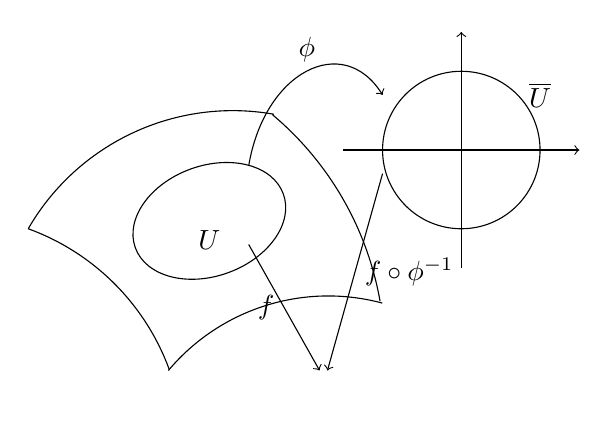
\begin{tikzpicture}
  \draw (0, 0) arc (150:80:3);
  \draw (3.1, 1.45) arc (50:10:4);
  \draw (0, 0) arc (70:20:3);
  \draw (1.78, -1.8) arc (140:75:2.65);

  \draw[rotate around={20:(2.3, 0.1)}] (2.3, 0.1) ellipse (1 and 0.7) node [below] {$U$};

  \draw[->] (4, 1)--(7, 1);
  \draw[->] (5.5, -0.5)--(5.5, 2.5);
  \draw (5.5, 1) circle (1);
  \node at (6.5, 1.7) {$\overline{U}$};
  \draw[->] (2.8, 0.8)..controls(3, 2)and(4, 2.5)..(4.5, 1.7) node [midway, above] {$\phi$};
  \draw[->] (4.5, 0.7)--(3.8, -1.8) node [midway, right] {$f\circ\phi^{-1}$};
  \draw[->] (2.8, -0.2)--(3.7, -1.8) node [midway, left] {$f$};
  \node at (3.75, -2) {$\R$};
\end{tikzpicture}
}
\end{wrapfigure}
Funkcja $f:M\to\R$ \important{wyrażona w mapie} $(U,\phi)$ to złożenie $f\circ\phi^{-1}:\overline{U}\to \R$.

\begin{definition}[funkcja $f:M\to\R$ jest gładka] Funkcja $f:M\to \R$ jest \important{gładka}, jeśli dla każdej mapy $(U, \phi)$ na $M$ $f\circ\phi^{-1}$ jest gładka.
\end{definition}

W tej definicji pojawia się pewien problem: dla jednej mapy $(U, \phi)$ $f$ może gładka, ale jeśli przejdziemy z obrazu mapy $(U, \psi)$ to może się okazać, że $f_2=f_1\circ\psi\circ\phi^{-1}$ nie jest gładka:

\begin{illustration}
  \draw (0, 0) arc (150:80:3);
  \draw (3.1, 1.45) arc (50:10:4);
  \draw (0, 0) arc (70:20:3);
  \draw (1.78, -1.8) arc (140:75:2.65);

  \draw[rotate around={20:(2.3, 0.1)}] (2.3, 0.1) ellipse (1 and 0.7) node [below] {$U$};

  \draw[->] (6, 1)--(9, 1);
  \draw[->] (7.5, -0.5)--(7.5, 2.5);

  \draw (7.5, 1) circle (1);
  \node at (8.5, 1.7) {$\overline{U}$};
  \draw[->] (2.8, 0.8)..controls(4, 2)and(5, 2.5)..(6.5, 1.7) node [midway, above] {$\phi$};
  \draw[->] (6.5, 0.5)--(2.9, -2.1) node [midway, right] {$f_1=f\circ\phi^{-1}$};
  \draw[->] (2.8, -0.2)--(2.8, -2) node [midway, left] {$f$};

  \draw[->] (-1, 1)--(-4, 1);
  \draw[->] (-2.5, -0.5)--(-2.5, 2.5);

  \draw (-2.5, 1) circle (1);
  \node at (-3.5, 1.7) {$\overline{\overline{U}}$};
  \draw[->] (-1.5, 0.5)--(2.7, -2.1) node [midway, left] {$f_2=f\circ\psi^{-1}$};
  \draw[->] (1.7, 0.5)..controls(1, 2)and(-1, 2.5)..(-1.5, 1.7) node [midway, above] {$\psi$};

  \node at (2.8, -2.3) {$\R$};

  \draw[<-] (-2, 2.3)..controls(0, 3.5)and(5, 3.5)..(7, 2.3) node [midway, above] {$\psi\circ\phi^{-1}$};
\end{illustration}

Dlatego chcemy móc założyć, że $\phi\circ\psi^{-1}$ jest przekształceniem gładkim.

\begin{definition}[zgodność map]
  Mapy $(U, \phi), (V, \psi)$ nazywamy (gładko) \important{zgodnymi}, gdy $\phi\circ\psi^{-1}$ i $\psi\circ\phi^{-1}$ są odwzorowaniami gładkimi.
\end{definition}

Odwzorowania $\phi\psi^{-1}$ nazywamy \acc[i]{odwzorowaniami przejścia} z jednej mapy do drugiej. Jeśli $\phi\psi^{-1}$ i $\psi\phi^{-1}$ są gładkie, to są one wzajemnie do siebie odwrotnymi bijekcjami. Takie odwzorowania nazywamy \acc[b]{dyfeomorfizmami} pomiędzy otwartymi podzbiorami $\R^n$. Zauważmy, że w każdym punkcie Jakobian, czyli wyznacznik macierzy pochodnych cząstkowych, jest dla dyfeomorfizmów niezerowy [ćwiczenia].

W ogólnym przypadku, gdy $U\cap V\neq \emptyset$, rysunek wygląda:
\begin{illustration}
  \draw (0, 0) arc (150:80:3);
  \draw (3.1, 1.45) arc (50:10:4);
  \draw (0, 0) arc (70:20:3);
  \draw (1.78, -1.8) arc (140:75:2.65);


  \filldraw[color=white, pattern=grid] (2.3, 0.65)--(2.4, 0.65)--(2.56, 0.55)--(2.57, 0.4)--(2.53, 0.3)--(2.3, 0.1)--(2.06, 0.3)--(2.03, 0.4)--(2.04, 0.55)--(2.2, 0.65)--cycle;
  \node at (2.3, 0.8) {$\scriptstyle U\cap V$};

  \draw[rotate around={20:(2, 0.3)}] (2, 0.3) ellipse (0.6 and 0.3);
  \node at (1.2, 0) {$V$};

  \draw[rotate around={-20:(2.6, 0.3)}] (2.6, 0.3) ellipse (0.6 and 0.3);
  \node at (3.4, 0) {$U$};

  \draw[color=white, pattern=grid] (7, 1)--(6.5, 1)--(6.6, 1.45)--(6.8, 1.75)--(7, 1.86)--cycle;
  \draw (7, 1) node [right, below] {$\scriptstyle\phi(U\cap V)$}--(7, 1.86);
  
  \draw[->] (6, 1)--(9, 1);
  \draw[->] (7.5, -0.5)--(7.5, 2.5);

  \draw (7.5, 1) circle (1);
  \node at (8.5, 1.7) {$\overline{U}$};
  \draw[->] (2.8, 0.5)..controls(4, 2)and(5, 2.5)..(6.5, 1.7) node [midway, above] {$\phi$};
  \draw[->] (6.6, 0.9)--(2.9, -2.1) node [midway, right] {$f_1=f\circ\phi^{-1}$};
  \draw[->] (2.8, -0.2)--(2.8, -2) node [midway, left] {$f$};

  \draw[color=white, pattern=grid] (-2, 1)--(-1.5, 1)--(-1.6, 1.45)--(-1.8, 1.75)--(-2, 1.86)--cycle;
  \draw (-2, 1)node [left, below] {$\scriptstyle\psi(U\cap V)$}--(-2, 1.86);

  \draw[->] (-1, 1)--(-4, 1);
  \draw[->] (-2.5, -0.5)--(-2.5, 2.5);

  \draw (-2.5, 1) circle (1);

  \node at (-3.5, 1.7) {$\overline{V}$};
  \draw[->] (-1.6, 0.95)--(2.7, -2.1) node [midway, left] {$f_2=f\circ\psi^{-1}$};
  \draw[->] (1.7, 0.5)..controls(1, 2)and(-1, 2.5)..(-1.5, 1.7) node [midway, above] {$\psi$};

  \node at (2.8, -2.3) {$\R$};

  \draw[<-] (-2, 2.3)..controls(0, 3.5)and(5, 3.5)..(7, 2.3) node [midway, above] {$\psi\circ\phi^{-1}:\phi(U\cap V)\to\psi(U\cap V)$};
\end{illustration}

  Mapy $(U, \phi)$ i $(V, \psi)$ nazywamy zgodnymi, jeśli:
  \begin{itemize}
    \item $U\cap V=\emptyset$
    \item odwzorowania przejścia 
      $$\phi\psi^{-1}:\psi(U\cap V)\to\phi(U\cap V)$$ 
      oraz 
      $$\psi\phi^{-1}:\phi(U\cap V)\to\psi(U\cap V)$$
      są gładkie ($\iff$ są dyfeomorfizmami podzbiorów $\phi(U\cap V)$ i $\psi(U\cap V)$).
  \end{itemize}

\begin{definition}[atlas gładki]
  \important{Gładkim atlasem} $\set{A}$ na rozmaitości $M$ nazywamy zbiór map $\{(U_\alpha, \phi_\alpha)\}$ takich, że:
  \begin{itemize}
    \item $\{U_\alpha\}$ pokrywają całe $M$
    \item każde dwie mapy z tego zbioru są zgodne.
  \end{itemize}
\end{definition}

\begin{example}
\item Rodzina map $\{(U_i^\pm, \phi_i^\pm)\}$ na sferze $S^n$ jest atlasem gładkim na $S^n$. Dla przykładu zbadamy zgodność map $(U_i^+,\phi_i^+)$ i $(U_j^+,\phi_j^+)$ dla $i<j$.

  Popatrzmy jak wyglądają interesujące nas zbiory:
  $$U_i^+\cap U_j^+=\{x\in S^n\;:\;x_i>0, x_j>0\}$$
  $$\phi_i^+(U_i^+\cap U_j^+)=\{x\in\R^n\;:\;|x|<1, x_{j-1}>0\}$$
  bo usuwamy $i$-tą współrzędną i numery poprzednich współrzędnych spadają o $1$ w dół,
  $$\phi_j^+(U_i^+\cap U_j^+)=\{x\in\R^n\;:\;|x|<1, x_i>0\}$$
  bo w tym przypadku usunęliśmy współrzędną na prawo od $i$, więc jej położenie nie zmienia się.
  \begin{figure}[h!]
    \begin{illustration}
      \filldraw[color=black, fill=blue!40] (-3, 0) arc (180:0:3cm);
      \filldraw[color=blue!40, fill=blue!40](-3, 0.02) arc (180:360:3cm and 1cm);
      \filldraw[color=black, fill=blue!40] (0, 3) arc (90:-90:3cm);
      \filldraw[color=blue!40, fill=blue!40] (0.02, 3) arc (90:270: 1cm and 3cm);
      \filldraw[color=black, fill=green!40] (3, 0) arc (0:90:3cm);
      \filldraw[color=black, fill=green!40] (0, 3) arc (90:200:1cm and 3cm);
      \filldraw[color=black, fill=green!40] (3, 0) arc (0:-110:3cm and 1cm);
      \filldraw[color=green!40, fill=green!40] (0, 3)--(3, 0)--(-1, -1)--cycle;

      \node at (3, 2) {$U_i^+\cap U_j^+$};

      \draw (0,0) circle (3cm);
      \draw (-3,0) arc (180:360:3cm and 1cm);
      \draw[dashed] (-3,0) arc (180:0:3cm and 1cm);
      \draw (0,-3) arc (270:90:1cm and 3cm);
      \draw[dashed] (0,3) arc (90:-90:1cm and 3cm);

      \filldraw[blue!40] (-4, -5) arc (180:90:1.5);
      \filldraw[blue!40] (-4, -5)--(-2.5, -5)--(-2.5, -3.5)--cycle;
      \filldraw[green!40] (-1, -5) arc (0:90:1.5);
      \filldraw[green!40] (-1, -5)--(-2.5, -5)--(-2.5, -3.5)--cycle;
      \draw[<-, thick] (-2.5, -3)--(-2.5, -7);
      \draw[->, thick] (-4.5, -5)--(-0.5, -5);
      \draw (-2.5, -5) circle (1.5);

      \filldraw[blue!40] (4, -5) arc (0:-90:1.5);
      \filldraw[blue!40] (4, -5)--(2.5, -5)--(2.5, -6.5)--cycle;
      \filldraw[green!40] (4, -5) arc (0:90:1.5);
      \filldraw[green!40] (4, -5)--(2.5, -5)--(2.5, -3.5)--cycle;
      \draw[<-, thick] (2.5, -3)--(2.5, -7);
      \draw[->, thick] (4.5, -5)--(0.5, -5);
      \draw (2.5, -5) circle (1.5);

      \node (j) at (3.3, -0.8) {$U_j^+$};
      \node (i) at (-1.5, 3.3) {$U_i^+$};

      \draw[->] (i)..controls(-4, 2.5)and(-5, -2)..(-4, -4) node [midway, left] {$\phi_i^+$};
      \draw[->] (j)..controls(4, -1)and(5, -2.5)..(4, -4) node [midway, right] {$\phi_j^+$};

    \draw[->] (3, -4.5)..controls(1.5, -3.5)and(-0.5, -3.5)..(-2, -4.5) node [midway, below] {$\phi_i^+(\phi_j^+)^{-1}$};
    \end{illustration}
  \end{figure}

  \begin{center}\begin{tikzcd}
    (x_1,...,x_n)\arrow[r, "(\phi_j^+)^{-1}"]\arrow[d, sloped, phantom, "\in"] & (x_1,....,x_{j-1}, \sqrt{1-|x|^2}, x_j,...,x_n)\arrow[d, "\phi_i^+"]\\
    \{x\in\R^n\;:\;|x|<1, x_i>0\}  & (x_1,...,x_{i-1}, \hat{x_i}, x_{i+1},...,x_{j-1},\sqrt{1-|x|^2}, x_j,...,x_n)\arrow[d, sloped, phantom, "\in"]\\
                                              & \{x\in\R^n\;:\;|x|<1, x_{j-1}>0\}
  \end{tikzcd}\end{center}
  Czyli odwzorowanie przejścia jest zadane wzorem:
  $$\phi_i^+(\phi_j^+)^{-1}(x_1,...,x_n)=(x_1,...,x_{i-1},x_{i+1},...,x_{j-1},\sqrt{1-|x|^2},x_j,...,x_n)$$
  i widać, że jest ono gładkie. Pozostałe rachunki przechodzą analogicznie.

    \item Jeśli $V$ jest przestrzenią liniową wymiaru $n<\infty$ nad $\R$, to dowolna norma określona na $V$ zadaje metrykę, która pozwala określić na $V$ topologię (identyczną dla równoważnych norm). Z taką topologią $V$ jest $n$-rozmaitością z naturalnie zdefiniowaną strukturą.

      Niech $(e_1,...,e_n)$ będzie bazą $V$. Rozważmy izomorfizm $E:\R^n\to V$ zadany przez
      $$E(x)=\sum_{i\leq n}x^ie_i.$$
      Funkcja ta w kontekście topologicznym jest homeomorfizmem, więc $(V, E^{-1})$ jest mapą na $V$. 

      Jeśli $(\overline{e}_1,...,\overline{e}_n)$ jest inną bazą na $V$, to mamy homeomorfizm 
      $$\overline{E}(x)=\sum x^j\overline{e}_j$$ 
      Istnieje wtedy pewna odwracalna macierz $(A_i^j)$ taka, że 
      $$e_i=\sum A^j_i\overline{j}$$ 
      dla każdego $i$. 

      Stąd modwzorowanie przejścia między tymi dwoma mapami jest zadana przez $\overline{E}^{-1}\circ E(x)=\overline{x}$, gdzie $\overline{x}=(\overline{x}^1,...,\overline{x}^n)$ jest zadane przez
      $$\sum_{j\leq n}\overline{x}^j\overline{e}_j=\sum_{i\leq n}x^ie_i=\sum_{i,j\leq n} x^iA_i^j\overline{e}_j\implies \overline{x}^j=\sum_{i\leq n} A_i^jx^i$$

      W takim razie jakakolwiek mapa wysyłająca $x$ na $\overline{x}$ jest odwracalna i liniowa $\implies$ jest dyfeomorfizmem. Stąd dowolne dwie mapy $(V, E)$ są gładko zgodne i ich rodzina definiuje na $V$ standardową gładką strukturę.
\end{example}

\begin{definition}[rozmaitość gładka]
  \important{Rozmaitością gładką} nazywamy parę $(M, \set{A})$, gdzie $M$ jest rozmaitością topologiczną, zaś $\set{A}$ jest pewnym atlasem gładkim na $M$.
\end{definition}

Zdarza się, że różne atlasy na tej samej rozmaitości topologicznej $M$ mogą zadawać tę samą rozmaitość gładką. Na przykład dla $M=\R^n$ istnieje atlas zawierający jedną mapę $\{(\R^n, id_{\R^n})\}$ oraz atlas $\{(B_x(r), id_{B_x(r)})\;:\;x\in\R^n, r>0\}$, który jest tak naprawdę "rozdrobnieniem" pierwszego atlasu. 

\begin{definition}[zgodność atlasów, mapy z atlasem]
  Niech $\set{A}$ będzie gładkim atlasem na $M$.

  \begin{enumerate}
    \item Mapa $(U, \phi)$ jest zgodna z $\set{A}$, jeśli jest zgodna z każdą mapą $(V, \psi)\in \set{A}$.
    \item Dwa atlasy $\set{A}_1, \set{A}_2$ na $M$ są zgodne, jeśli każda mapa z $\set{A}_1$ jest zgodna z $\set{A}_2$.
  \end{enumerate}
\end{definition}

Warto zaznaczyć, że zgodność atlasów jest relacją zwrotnią i przechodnią [ćwiczenia]. Zgodne atlasy zadają tę samą strukturę rozmaitości gładkiej na topologicznej rozmaitości $M$. Wszystkie zgodne atlasy należą do jednego większego atlasu, co było przyczyną powstania definicji atlasu maksymalnego.

\begin{definition}[atlas maksymalny]
  $\set{A}$ jest \important{atlasem maksymalnym} na rozmaitości $M$, jeśli każda mapa zgodna z $\set{A}$ należy do $\set{A}$.
\end{definition}

Każdy atlas $\set{A}$ na $M$ zawiera się w dokładnie jednym atlasie maksymalnym, złożonym ze wszystkich map zgodnych z $\set{A}$ [ćwiczenia]. Dodatkowo, zgodne atlasy zawierają się w tym samym atlasie maksymalnym. Wtedy można definiować rozmaitość gładką jako parę $(M, \set{A})$, gdzie $M$ jest rozmaitością topologiczną, a $\set{A}$ jest pewnym gładkim atlasem maksymalnym.
\bigskip

\textbf{Dopowiedzenie o funkcjach gładkich}

Funkcja $f:M\to\R$ jest gładka względem atlasu $\set{A}$ na $M$, jeśli dla każdej mapy $(U, \phi)\in\set{A}$ $f\circ\phi^{-1}$ jest gładka.

\begin{fact}[gładkość względem atlasu]$ $\newline
  \begin{itemize}
    \item Jeśli $f:M\to\R$ jest gładka względem $\set{A}$, zaś $(U, \phi)$ jest mapą zgodną z $\set{A}$, to $f\circ\phi^{-1}$ jest gładka.
    \item Jeśli $\set{A}_1$ i $\set{A}_2$ są zgodnymi atlasami, to $f:M\to\R$ jest gładka względem $\set{A_1}$ $\iff$ $f$ jest gładka względem $\set{A}_2$ $\iff$ $f$ jest gładka względem atlasu maksymalnego $\set{A}_{max}$ zawierającego $\set{A}_1$ i $\set{A_2}$.
  \end{itemize}
\end{fact}
\begin{proof}
  Ćwiczenia
\end{proof}

\subsection{Warianty pojęcia rozmaitości różniczkowalnej}

Mówimy, że mapy $(U,\phi),(V, \psi)$ są \acc[i]{$C^k$-zgodne} jeśli $\phi\circ\psi^{-1}$ i $\psi\circ\phi^{-1}$ są funkcjami klasy $C^k$ (posiadają pochodne cząstkowe rzędów $\leq k$). $C^k$-atlas to z kolei rodzina $C^k$-zgodnych map, która określa strukturę $C^k$-rozmaitości na $M$. Struktura $C^k$-rozmaitości jest słabsza niż rozmaitości gładkiej i nie da się na niej zdefiniować map klasy $C^m$ dla $m>k$.

$C^0$ rozmaitość to określenie na rozmaitość topologiczną, a $C^\infty$-rozmaitość jest tym samym co rozmaitość gładka.
\medskip

\textbf{Dychotomia $C^0$ i $C^k$ dla $k>0$} aka dykresja

Z każdego maksymalnego atlasu $C^1$-rozmaitości można wybrać atlas złożony z map $C^\infty$-zgodnych. Zatem, każda $C^1$-rozmaitość posiada $C^1$-zgodną strukturę $C^\infty$-rozmaitości [Whitney, 1940]. Istnieją jednak $C^0$-rozmaitości, które nie dopuszczają żadnej zgodnej struktury gładkiej [Quinn '82, Friedmann '82].
\medskip

\begin{itemize}[leftmargin=*]
  \item Na rozmaitości analitycznej mapy są analitycznie zgodne $[C^\omega]$. Mapy są analitycznie zgodne, gdy wyrażają się za pomocą szeregów potęgowych.
  \item Rozmaitość zespolona ma mapy będące funkcjami w $\C^n$ zamiast $\R^n$.
  \item W rozmaitości konforemnej mapy zachowują kąty między punktami.
  \item Istnieją też rozmaitości kawałkami liniowe (PL)...
\end{itemize}

\subsection{Różniczkowalność odwzorowań rozmaitości}

\begin{definition}[odwzorowanie $C^k$-różniczkowalne]
Dla $M, N$ gładkich rozmaitości i $f:M\to N$ ciągłej mówimy, że $f$ jest \important{$C^k$-różniczkowalna} w punkcie $p$, jeśli dla dowolnych map $(U,\phi)\ni p$ oraz $(V,\psi)\ni f(p)$ złożenie
$$\psi\circ f\circ\phi^{-1}:\phi[U\cap f^{-1}(V)]\to \psi(V)$$
jest $C^k$-różniczkowalne w punkcie $\phi(p)$.
\end{definition}

\begin{illustration}
  \node at (0,0) {ZRÓB RYSUNEK};
\end{illustration}

\subsection{Definiowanie rozmaitości gładkiej $X$ za pomocą samego atlasu}

\begin{lemma}
  Niech $X$ będzie zbiorem (bez zadanej topologii) i $\{U_\alpha\}$ będzie kolekcją podzbiorów w $X$ taką, że dla każdego $\alpha$ istnieje $\phi_\alpha:U_\alpha\to\R^n$ różniczkowalne takie, że
  
  \begin{enumerate}
    \item dla każdego $\alpha$ $\phi_\alpha(u_\alpha)=\overline{U_\alpha}\subseteq\R^n$ jest otwarty
    \item dla dowolnych $\alpha, \beta$ $\phi_\alpha(U_\alpha\cap U_\beta)$ oraz $\phi_\beta(U_\alpha\cap U_\beta)$ są otwarte w $\R^n$.
    \item jeśli $U_\alpha\cap U_\beta\neq\emptyset$, to $\phi_\beta\circ\phi_\alpha^{-1}:\phi_\alpha(U_\alpha\cap U_\beta)\to\phi_\beta(U_\alpha\cap U_\beta)$ jest gładkie (a nawet dyfeomorficzne, bo odwzorowanie odwrotne $\phi_\alpha\circ\phi_\beta^{-a}$ też jest gładkie)
    \item przeliczalnie wiele spośród $U_\alpha$ pokrywa $X$
    \item dla każdego $p, q\in X$, jeśli $p\neq q$, to istnieją $\alpha, \beta$ oraz otwarte $V_p\subseteq\overline{U_\alpha}$ i $V_q\subseteq\overline{U_\beta}$ takie, że $p\in \phi_\alpha^{-1}(V_p), q\in\phi_\beta^{-1}(V_q)$ oraz $\phi_\alpha^{-1}(V_p)\cap\phi_\beta^{-1}(V_q)=\emptyset$ (oddzielanie punktów otwartymi zbiorami mapowymi).
  \end{enumerate}

  Wówczas na $X$ istnieje jedyna struktura rozmaitości topologicznej, dla której zbiory $U_\alpha$ są otwarte. Ponadto rodzina $\{(U_\alpha, \phi_\alpha)\}$ tworzy wtedy gładki atlas na $X$.
\end{lemma}

\begin{proof}
  A dokładniej szkic dowodu. \marginpar{Dokładny dowód w Lee, lemat 1.35.}

  Określimy topologię na $X$ przy pomocy przeciwobrazów przez $\phi_\alpha$ otwartych podzbiorów $\overline{U_\alpha}=\phi_\alpha(U_\alpha)\subseteq\R^n$. Sprawdzenie, że jest to bazą topologii jest ćwiczeniem. Dzięki temu zbadanie lokalnej euklidesowości jest trywialne.

  Dzięki warunkowi 4 nietrudno jest wybrać wtedy bazę przeliczalną [ćwiczenie], a warunek Hausdorffowości wynika z 5.
\end{proof}

\begin{example}
\item $\set{L}$ jest zbiorem prostych na płaszczyźnie. Na takim zbiorze nie ma dogodnej topologii, którą możnaby od razu wykorzystać. Zdefiniujmy zbiory:
  $$U_v=\{\text{proste niepoziome}\}$$
  $$U_h=\{\text{proste niepionowe}\}$$
  oraz funkcje $\phi_h, \phi_v$:
  $$U_h\ni L=\{y=ax+b\}\overset{\phi_h}{\mapsto} (a, b)\in\R^2$$
  $$U_v\ni L=\{x=cy+d\}\overset{\phi_v}{\mapsto} (c, d)\in\R^2$$
  Obie te funkcje są różnowartościowe i ich obrazy to $\R^2$, czyli warunek 1 jest spełniony. Ponieważ jest ich tylko 2 sztuki i pokrywają całęgo $X$, to również 4. został spełniony. Sprawdźmy teraz 2:
  $$U_h\cap U_v=\{\text{proste niepionowe i niepoziome}\}=\{y=ax+b\;:\;a\neq 0\}=\{x=cy+d\;:\;c\neq0\}$$
  $$\phi_h(U_h\cap U_v)=\{(a, b)\in\R^2\;:\;a\neq 0\}$$
  $$\phi_v(U_h\cap U_v)=\{(c, d)\;:\;c\neq0\}$$
  są otwarte, więc 2 jest spełniona. Teraz kolej na 3.
  
  Weźmy prostą $L=\{x=cy+d\}=\{y=\frac{1}{c}x-\frac{d}{c}\}\in U_h\cap U_v$. 
  \begin{center}\begin{tikzcd}
    \left(\frac{1}{c},-\frac{d}{c}\right) & \arrow[l, "\phi_h" above]L\arrow[r, "\phi_v"] & (c, d)
  \end{tikzcd}\end{center}
  Zatem $\phi_h\phi_v^{-1}(c, d)=\left(\frac1c,-\frac{d}{c}\right)$ jest gładkie (podobnie $\phi_v\phi_h^{-1}$).

  Warunek 5. jest łatwy do sprawdzenia [ćwiczenie].

  Z tą naturalną (mimo wszystko) topologią $\set{L}$ jest w istocie homeomorficzne z wnętrzem wstęgi M\"obiusa. Stąd do opisania $\set{L}$ nie wystarcza jedna mapa.
\end{example}
\bigskip

\textbf{O notacjach:}

\begin{itemize}
  \item W dalszej części rozważań będziemy utożsamiać mapowe otoczenie $U\subseteq M$ z obrazem przez mapę, czyli $\overline{U}=\phi(U)\subseteq\R^n$. Można o tym myśleć, że przenosimy siatkę współrzędnych $(x_1,...,x_n)$ z $\overline{U}$ przez $\phi^{-1}$ na $U\subseteq M$.
  \item Za pomocą translacji współrzędnych zawsze możemy przyjąć, że $p=(0,...,0)$ w mapie, czyli możemy założyć, że $(U,\phi)$ jest mapą o początku w $p$.
  \item Często będziemy przechodzić do mniejszych zbiorów mapowych, za mapę biorąc odwzorowanie obcięte (jest to mapa zgodna z atlasem). Będziemy wtedy mówić, że przyjmujemy, iż mapa wokół $p$ ma zbiór mapowy tak mały, jak nam akurat potrzeba, np. że jest rozłączny z pewnym zbiorem domkniętym $F\subseteq M$ niezawierającym $p$.
\end{itemize}

\subsection{Rozmaitość gładka z brzegiem}

\begin{bbox}
Rzeczywistą półprzestrzeń oznaczamy
$$H^n=\{(x_1,...,x_n)\in\R^n\;:\;x_n\geq 0\},$$
jej brzegiem nazywamy
$$\partial H^n=\{(x_1,...,x_n)\in\R^n\;:\;x_n=0\}$$
a wnętrzem:
$$int(H^n)=\{(x_1,..., x_n)\in\R^n\;:\;x_n>0\}.$$

Dla $U\subseteq H^n$ oznaczymy $\partial U=U\cap \partial H$ oraz $int(U)=U\cap int(H^n)$, czyli definicja brzegu i wnętrza jest nieco inna niż na topologii. Użyjemy $H^n$ oraz definicji jej brzegu i wnętrza, by zdefiniować rozmaitość gładką z brzegiem.
\end{bbox}

Dla $U\subseteq H^n$ otwartego i $f:U\to\R^m$ mówimy, że $f$ jest \important{gładka}, gdy jest obcięciem do $U$ gładkiej funkcji $\hat{f}:\hat{U}\to\R^m$, $\hat{U}\subseteq\R^n$ otwartego, $U\subseteq\hat{U}$. \emph{Pochodne cząstkowe funkcji $f$ są dobrze określone na $int(U)$, a ponieważ są ciągłe, to są również dobrze określone na $\partial U$} (tzn. nie zależą od wyboru rozszerzenia $\hat{f}$). Z analizy matematycznej wiemy, że rozszerzenia $\hat{f}$ istnieje $\iff$ wszystkie pochodne cząstkowe $f$ w $int(U)$ w sposób ciągły rozszerzają się do $\partial U$.

\begin{definition}[rozmaitość z brzegiem]
  $M$ jest \important{gładką rozmaitością z brzegiem}, jeśli posiada atlas $\{(U_\alpha,\phi_\alpha)\}$, $U_\alpha\subseteq M$ i $\phi_\alpha:U_\alpha\to H^n$ i $\overline{U_\alpha}=\phi_\alpha(U_\alpha)$ jest otwarty w $H^n$, gdzie odwzorowania przejścia są gładkie (tzn. $\phi_\alpha\phi_\beta^{-1}$ są dyfeomorfizmami pomiędzy otwartymi podzbiorami w $H^n$).
\end{definition}

\begin{illustration}
  \draw[rounded corners=35pt](7,-1)--(4.2,-1)--(2,-2)--(0,0) -- (2,2)--(4.2,1)--(7,1);
  \draw (1.5,0.2) arc (175:315:1cm and 0.5cm);
  \draw (3,-0.28) arc (-30:180:0.7cm and 0.3cm);
  \filldraw[color=blue, fill=blue!40] (6.4, 0) circle (0.6);
  \filldraw[color=black, fill=blue!40!black!60] (7.5,0) arc (0:360:0.5cm and 1cm);
  %\node (a) at (20:2.5) {$M$};
  %\node (a) at (-12:7.5) {$\partial M=N$};
  \filldraw[color=blue, fill=blue!40] (4.5, 0.35) circle (0.6);

  \filldraw[color=blue, fill=blue!40] (8.4, -0.2) circle (0.5);
  \filldraw [color=blue, fill=blue!40] (8.8, -1.5) arc (180:0:0.5);

  \draw[<-] (9, 0.5)--(9, -1.7);
  \draw[->] (7.5, -1.5)--(10.5, -1.5);

  \draw[->, white, very thick] (5, 0.4)..controls(5.5, 1.5)and(7.5, 1.3)..(8, 0);
  \draw[->, white, very thick] (6.2, -0.5)..controls(6.5, -1.5)and(8, -2)..(8.8, -1.3);

  \draw[->] (5, 0.4)..controls(5.5, 1.5)and(7.5, 1.3)..(8, 0);
  \draw[->] (6.2, -0.5)..controls(6.5, -1.5)and(8, -2)..(8.8, -1.3);

  \node at (9.4, 0.3) {$H^n$};
\end{illustration}

\begin{fact}[raz w brzegu, zawsze w brzegu]
  Jeśli w pewnej mapie $(U_\alpha,\phi_\alpha)$, $\phi_\alpha(p)\in\partial H^n$, to w każdej innej mapie $(U_\beta, \phi_\beta)$ zawierającej $p$ $\phi_\alpha(p)\in\partial H^n$.
\end{fact}

\begin{proof}
  Wynika to z twierdzenia o odwzorowaniu otwartym, wraz z nieosobliwością Jakobianu odwzorowań przejścia. 

  Dla rozmaitości topologicznych z brzegiem analogiczny fakt wymaga w dowodzie twardego twierdzenia Brouwera o niezmienniczności obrazu - analogicznego twierdzenia o odwzorowaniu otwartym dla ciągłych injekcji.
\end{proof}

\begin{definition}[brzeg, wnętrze]
  \important{Brzegiem} $n$-rozmaitości $M$ z brzegiem nazywamy zbiór
  $$\partial M=\{p\in M\;:\;\text{w pewnej (każdej) mapie }p\in(U_\alpha,\phi_\alpha)\text{ zachodzi }\phi(p)\in\partial H^n$$
    wnętrze $M$ nazywa się
    $$int(M)=\{p\in M\;:\;(\exists\;(U_\alpha,\phi_\alpha)\;\phi_\alpha(p)\in int(H^n)\}$$
\end{definition}

  \begin{fact}
    Wnętrze $int(M)$ $n$-rozmaitości gładkiej $M$ jest $n$-rozmaitością bez brzegu.
  \end{fact}

  \begin{proof}
    Jako atlas bierzemy $\{(U_\alpha',\phi_\alpha')\}$, gdzie 
    $$U_\alpha'=\phi_\alpha^{-1}(int(\overline{U_\alpha}))=U_\alpha\cap int(M),\quad\phi_\alpha'=\phi_\alpha\restriction U_\alpha'$$
    Odwzorowania przejścia $\phi_\alpha'(\phi_\beta')^{-1}$ są obcięciami $\phi_\alpha\phi_\beta^{-1}$, więc są gładkie.
  \end{proof}

\begin{example}
\item Dysk $D^n=\{x\in\R^n\;:\;|x|\leq 1\}$ jest $n$-rozmaitością z brzegiem $\partial D^n=S^{n-1}=\{x\in\R^n\;:\;|x|=1\}$.

  \begin{proof}
    Skonstruujemy mapy, pomijając sprawdzanie gładkości odwzorowań przejścia.

    Mapa $(U_0, \phi_0)$:
    $$U_0=\{x\;:\;|x|<1\},\;\phi_0:U_0\to H^n,\;\phi_0(x_1,...,x_n)=(x_1,...,x_{n-1}, x_n+2)$$

    Mapy $(U_i^\pm,\phi_i^\pm)$

    \begin{illustration}
      \filldraw[green!40] (0, 1.5) arc (90:-90:1.5);
      \draw (0, 0) circle (1.5);
      \draw (1.5, -2)--(1.5, 2);
      \filldraw (0.8, -0.5) circle (1.5pt) node [below] {p};
      \draw (0, 0)--(1.5, -0.95);
      \filldraw (1.5, -0.95) circle (1.5pt) node [right] {$\pi(p)$};
      \filldraw (0,0)circle(1.5pt);
      \draw(0, 1.5)--(0, -1.5);
      \node at (3, -1.5) {$\R^{n-1}=\{x_i=1\}$};
      \node at (-1, -1.5) {$D^n$};
      \node (a) at (-0.5, 2) {$U_i^\pm$};
      \draw (-0.3, 1.8)--(0.4, 1);
    \end{illustration}
    $$U_i^+=\{x\in D^n\;:\;x_i>0\}$$
    $$U_i^-=\{x\in D^n\;:\;x_i < 0\}$$
    $$\phi_i^\pm(x_1,...,x_n)=\left(\frac{x_1}{x_i},...,\frac{x_{i-1}}{x_i},\frac{x_{i+1}}{x_i},...,\frac{x_n}{x_i},\underbrace{1-\sum x_i^2}_{1-r^2}\right)$$
    $$\phi_i^\pm(p)=(\pi(p),1-r^2)\in H^n$$
  \end{proof}
\item Inny atlas na $D^n$, składający się tylko z dwóch map:
  \begin{illustration}
    \node[rectangle, shading=axis, left color=white, right color=blue!15, shading angle=90, anchor=north, minimum width=5cm, minimum height=4cm] at (-2.5, 2) {};

    \node[rectangle, shading=axis, left color=white, right color=yellow!20, shading angle=-90, anchor=north, minimum width=5cm, minimum height=4cm] at (4, 2) {};
    \node at (3.5, -1.5) {$\color{yellow}H_A^n$};

    \node at (-2, -1.5) {$\color{blue}H_B^n$};
    \draw (0, 0) circle (1.5);
    \draw (1.5, 0) circle (1.5);
    \draw (0, 2)--(0, -2);
    \draw (1.5, 2)--(1.5, -2);
    \filldraw[color=black, fill=orange!20] (0.75, 0) circle (0.75);
    \node at (1.3, -0.75) {$D^n$};

    \filldraw (0, 0) circle (1.5pt) node [left] {$A$};
    \filldraw (1.5, 0) circle (1.5pt) node [right] {$B$};
  \end{illustration}
  Niech $A$ i $B$ będą punktami styczności dwóch prostych równoległych do dysku $D^n$. Rozważmy zbiory
  $$U_A=D^n\setminus\{A\}$$
  $$U_B=D^n\setminus\{B\}$$
  oraz odwzorowania $\phi_A:U_A\to H_A^n$ i $\phi_B:U_B\to H_B^n$ będące inwersjami dysku względem sfer $S^n$ o środkach w $A$ i $B$ oraz promieniu $2$.
\item Tutaj warto zaznaczyć, że jeśli $n=0$, to wtedy $\partial M=\emptyset$ i $M$ jest $0$-rozmaitością. W dodatku, zbiór rozmaitości gładkich z brzegiem można rozumieć jakoby zawierał zbiór rozmaitości topologicznych, gdyż $\partial M=\emptyset\iff M$ jest rozmaitością topologiczną.
\end{example}

\newpage
%
\section{Rozkład jedności}

Rozważmy rozmaitość z brzegiem $M$. \marginpar{Bardziej ogólnie, możemy chcieć dla dowolnego zbioru domkniętego $D\subseteq M$ znaleźć funkcję, która dla $p\in D$ jest równa zero, a na $M\setminus D$ ma wartości ściśle dodatnie.}Chcielibyśmy mieć narzędzie, które pozwoli nam tworzyć gładkie funkcje $f:M\to\R$ takie, że $f(p)=0$ gdy $p\in\partial M$ oraz $f(p)>0$ dla dowolnego $p\in Int(M)$.

\begin{illustration}
  \filldraw[color=green, fill=green!30, rotate around={20:(7, -0.5)}] (7, -0.5) arc (300:30:0.7 and 0.5);

  \filldraw[color=green, fill=green!30] (9.5,0.5) arc (180:0:0.5);
  \draw[->] (9, 0.5)--(11, 0.5);
  \draw[->] (10, -0.5)--(10, 1.5) node [right] {$\scriptstyle x_n$};

  \draw[rounded corners=35pt](7,-1)--(4.2,-1)--(2,-2)--(0,0) -- (2,2)--(4.2,1)--(7,1);
  \draw (1.5,0.2) arc (175:315:1cm and 0.5cm);
  \draw (3,-0.28) arc (-30:180:0.7cm and 0.3cm);
  \filldraw[color=black, fill=white] (7.5,0) arc (0:360:0.5cm and 1cm);
  \node (a) at (20:2.5) {$M$};
  \node (a) at (-12:7.5) {$\partial M$};

  \draw[->] (6.3, -0.5)..controls(7, -1)and(8, -0.5)..(9.7, 0.6) node [midway, above] {$\phi$};
\end{illustration}

Lokalnie, na zbiorze mapowym $(U_\alpha,\phi)$ możemy funkcję spełniającą wymagania wyżej zadać przy pomocy funkcji wychodzącej z $\overline{U_\alpha}=\phi(U_\alpha)$
$$f_\alpha:\overline{U_\alpha}\to\R,\quad f(x_1,...,x_n)=x_n,$$
gdyż ostatnia współrzędna punktów z $\partial M$ jest zawsze zerowa (gdyż są one w $\partial H^n$). Stąd w prosty sposób dostajemy funkcję:
$$f_\alpha:U_\alpha\to\R,\quad f_\alpha=\overline{f_\alpha}\circ \phi$$
która lokalnie spełnia nasze wymagania. Nie możemy jednak w prosty sposób przełożyć lokalne $f_\alpha$ na funkcję $f:M\to\R$. 

\subsection{Lokalnie skończone rozdrobnienie}

Przypomnijmy definicje, które będą przydatne przy rozkładach jedności:

\begin{definition}[pokrycie lokalnie skończone] Pokrycie $\{A_\alpha\}$ podzbiorami przestrzeni topologicznej $X$ jest \important{lokalnie skończone}, jeśli dla każdego $p\in X$ istnieje otoczenie $U_p$ takie, że $U_p\cap A_\alpha\neq\emptyset$ tylko dla skończenie wielu $\alpha$.
\end{definition}

\begin{definition}[rozdrobnienie] Pokrycie $\{V_\beta\}$ przestrzeni $X$ zbiorami otwartymi nazywamy \important{rozdrobnieniem pokrycia} $\{U_\alpha\}$, jeśli każdy $V_\beta$ zawiera się w pewnym $U_\alpha$.
\end{definition}

Warto nadmienić, że relacja bycia rozdrobnieniem jest przechodnia.\marginpar{$\{W_\gamma\}\prec\{V_\beta\}\prec\{U_\alpha\}\implies\;\implies\{W_\gamma\}\prec\{U_\alpha\}$} Będziemy oznaczać ją przez $\{V_\beta\}\prec\{U_\alpha\}$.

\begin{definition}[przestrzeń parazwarta] Przestrzeń topologiczna $X$ jest \important{parazwarta}, jeśli każde jej pokrycie $\{U_\alpha\}$ zbiorami otwartymi posiada lokalnie skończone rozdrobnienie $\{V_\beta\}$.
\end{definition}

Warto przypomnieć, że każda rozmaitość topologiczna jest parazwarta. \marginpar{Dowód: patrz Lee strona 36-37}Dowód tego lematu wykorzystuje w istotny sposób lokalną zwartość, czyli istnienie dla każdego punktu otoczeń prezwartych (po domknięciu zwartych). Własność ta została udowodniona na ćwiczeniach.

\begin{remark}\label{uwaga:2.4}
Rozdrobnienie wynikające z parazwartości rozmaitości topologicznych można z góry uznać za składające się z prezwartych zbiorów mapowych.
\end{remark}

\begin{proof}
Niech $\{U_\alpha\}$ będzie pokryciem $M$. Łatwo jest znaleźć rozdrobnienie $\{U'_\gamma\}\prec\{U_\alpha\}$ złożone ze zbiorów prezwartych mapowych. Wystarczy obraz każdego $U_\alpha$ w $\R^n$ pokryć zbiorami prezwartymi i wrócić z nimi na $M$. Z faktu, że rozmaitości są parazwarte dostajemy lokalnie skończone rozdrobnienie $\{V_\beta\}\prec\{U'_\gamma\}$, które z przechodności $\prec$ jest też rozdrobnieniem $\{U_\alpha\}$. Dodatkowo, każdy $V_\beta$ zawiera się w pewnym $U'_\gamma$, które były mapowe i prezwarte, więc i $V_\beta$ taki jest.
\end{proof}

\begin{remark}
  Niech $\{A_\alpha\}$ będzie lokalnie skończoną rodziną parazwartych podzbiorów rozmaitości $M$. Wtedy dla każdego $A_{\alpha_0}$ podrodzina
  $$\{A_\alpha\;:\;A_\alpha\cap A_{\alpha_0}\neq\emptyset\}$$
  jest skończona.
\end{remark}

\begin{proof}
  Załóżmy nie wprost, że dla pewnego $A_{\alpha_0}$ podrodzina $\{A_\alpha\;:\;A_\alpha\cap A_{\alpha_0}\neq\emptyset\}$ jest nieskończona. Możemy w takim razie wybrać z niej ciąg $A_{\alpha_i}$ oraz ciąg punktów $x_i\in A_{\alpha_i}\cap A_{\alpha_0}$. Ciąg $x_i$ ma punkt skupienia w pewnym $p\in cl(A_{\alpha_0})$. 

  Ponieważ $p$ jest punktem skupienia $x_i$, to dowolne otwarte otoczenie $U_p$ punktu $p$ zawiera nieskończenie wiele elementów $x_i$. W takim razie $U_p$ przecina się z nieskończenie wieloma zbiorami $A_\alpha$. Jest to sprzeczne z lokalną skończonościa $\{A_\alpha\}$.
\end{proof}

W uwadze \ref{uwaga:2.4} pokazaliśmy mapowość i prezwartość zbiorów z rozdrobnienia $\{V_\beta\}$ wynikającego z parazwartości rozmaitości topologicznych. Możemy teraz dodatkowo zapewnić sobie istnienie interesujących nas zbiorów zwartych:

\begin{remark}
  Niech $\{V_\beta\}$ będzie lokalnie skończonym rozdrobnieniem pokrycia $M$ składającym się ze zbiorów mapowych. Wtedy dla każdego $\beta$ istnieje zwarty zbiór $D_\beta\subseteq V_\beta$ taki, że
  $$\bigcup D_\beta=M$$
  to znaczy możemy wybrać "rozdrobnienie" przy pomocy zwartych zbiorów, które nadal pokrywa $M$.
\end{remark}

\begin{proof}
  Ponieważ $V_\beta$ są zbiorami mapowymi, to o każdym z nich możemy myśleć jak o otwartym podzbiorze w $\R^n$ poprzez utożsamienie go z otwartym zbiorem $\overline{V_\beta}=\phi_\beta(V_\beta)$ dla mapy $(V_\beta, \phi_\beta)$.
\end{proof}

\newpage
%
\section{Dyskretne ilorazy rozmaitości}

\subsection{Klejenie rozmaitości wzdłuż brzegu}

\subsection{Dopiero teraz całe mięso}

\newpage
%
\section{Wektory styczne}

\textbf{Oznaczenia z analizy matematycznej:}
\begin{itemize}
  \item dla gładkiej funkcji $f:(a, b)\to\R^n$ takiej, że $f=(f_1,...,f_n)$ i dla $t\in (a, b)$ pochodną nazywamy wektor
    $$f'(t)=\frac{\partial f}{\partial t}(t)=\begin{pmatrix}f_1'(t)\\f_2'(t)\\...\\f_n'(t)\end{pmatrix}$$
  \item dla gładkiego odwzorowania $f:U\to\R^m$, $U\subseteq \R^n$ i $p\in U$ oznaczamy macierz pierwszych pochodnych cząstkowych w punkcie $p$ przez $D_pf$. Dokładniej, jeśli $f=(f_1,...,f_m)$ i $f_i:U\to\R^m$ są wszystkie gładkie, to
    $$D_pf=\begin{pmatrix}\frac{\partial f_1}{\partial x_1}(p) & \frac{\partial f_1}{\partial x_2}(p) & \hdots & \frac{\partial f_1}{\partial x_n}(p)\\
      \vdots & \vdots & \vdots & \vdots\\
    \frac{\partial f_m}{\partial x_1}(p) & \frac{\partial f_m}{\partial x_2}(p) & \hdots & \frac{\partial f_m}{\partial x_n}(p) \end{pmatrix}$$
    Tym samym symbolem oznaczamy też odwzorowanie liniowe $\R^n\to\R^m$ zadane tą macierzą (różniczka $f$ w $p$).
\end{itemize}

\subsection{Przestrzeń styczna - definicja kinematyczna}

Przestrzeń styczną będziemy definiować przez styczność krzywych gładkich.
\marginpar[]{J.M. Lee definiuje przestrzeń styczną przy pomocy derywacji oraz przedstawia możliwość użycia m.in. kiełków funkcji gładkich}

Niech $M$ będzie gładką rozmaitością. \acc[b]{Krzywą gładką} na $M$ nazywamy gładkie odwzorowanie $c:(a, b)\to M$. O krzywej gładkiej $c$ takiej, że $c(t_0)=p$ mówimy, że jest \acc[i]{zbazowana w $p$}. Zbiór par $(c, t_0)$ krzywych zbazowanych w $p$ oznaczamy ${\color{green}C_pM}$.


\begin{definition}[styczność krzywych w mapie]
  Niech $\phi:U\to \R^n$ będzie mapą wokół $p$. Krzywe $(c_1,t_1)$ i $(c_2, t_2)$ zbazowane w $p$ są do siebie styczne w mapie $(U,\phi)$ jeśli $(\phi\circ c_1)'(t_1)=(\phi\circ c_2)'(t_2)$.
\end{definition}

\begin{lemma}[styczność w jednej mapie $\iff$ styczność w każdej mapie]
  Jeżeli $(c_1,t_1),(c_2,t_2)\in C_pM$ są styczne w mapie $(U,\phi)$ wokół $p$, to są też styczne w dowolnej innej mapie $(W, \psi)$ wokół $p$ (zgodnej z $(U, \phi)$.
\end{lemma}

\begin{proof}
  \begin{align*}
    (\psi\circ c_1)'(t_1)&=[(\psi\circ\phi^{-1})\circ(\phi\circ c_1)(t_1)]'=D_{\phi(p)}(\psi\circ\phi^{-1})\circ [(\phi\circ c_1)'(t_1)]=\\
                         &=D_{\phi(p)}(\psi\circ\phi^{-1})[(\phi\circ c_2)'(t_2)]=[(\psi\circ\phi^{-1})\circ(\phi\circ c_2)(t_2)]'\\
                         &=(\psi\circ c_2)'(t_2)
  \end{align*}
\end{proof}

\begin{definition}[styczność krzywych]
  Krzywe $(c_1,t_1),(c_2,t_2)\in C_pM$ są styczne, jeżeli są styczne w pewnej (równoważnie każdej) mapie wokół $p$.
\end{definition}

Relacja styczności krzywych jest relacją równoważności na $C_pM$, bo jest zwrotnia, symetryczna i przechodnia ($(\phi\circ c_1)'(t_1)=(\phi\circ c_2)'(t_2)\text{ i }(\phi\circ c_2)'(t_2)=(\phi\circ c_3)'(t_3)\implies(\phi\circ c_1)'(t_1)=(\phi\circ c_3)'(t_3)$).

\begin{definition}[przestrzeń styczna]
  \important{Przestrzenią styczną} do $M$ w punkcie $p$ nazywamy zbiór klas abstrakcji relacji styczności krzywych zbazowanych w $p$
  $$T_pM:=C_pM/stycznosc$$
  Klasę abstrakcji krzywej $(c, t_0)\in C_pM$ oznaczamy przez $[c, t_0]$ lub $c'(t_0)$. Elementy przestrzeni $T_pM$ nazywamy \acc[b]{wektorami stycznymi} do $M$ w punkcie $p$.
\end{definition}

\subsection{Struktura wektorowa przestrzeni $T_pM$}

Dla mapy $\phi:U\to \R^n$ wokół $p\in M$ określamy dwa odwzorowania:
\marginpar{Odwzorowanie $\phi_p^*$ jest dobrze określone z definicji $T_pM$ (wszystkie krzywe z jednej klasy abstrakcji mają tę samą pochodną w jednej mapie).}
\phantomsection\label{phi z gwiazdka}
\begin{align*}
  &\phi_p^*:T_pM\to\R^n\quad\; \phi_p^*([c, t_0])=(\phi\circ c)'(t_0)\in \R^n\\
  &\lambda_{\phi,p}:\R^n\to T_pM\quad \lambda_{\phi,p}(v)=[c_v, 0]
\end{align*}
gdzie $c_v(t)=\phi^{-1}(\phi(p)+tv)$.

\begin{lemma}
  $\phi^*_p\circ\lambda_{\phi, p}=id_{\R^n}$ oraz $\lambda_{\phi, p}\circ\phi_p^*=id_{T_pM}$, czyli $\phi_p^*$ i $\lambda_{\phi,p}$ są one wzajemnie jednoznacze i do siebie odwrotne.
\end{lemma}

\begin{proof}
  Niech $v\in\R^n$, wtedy
  \begin{align*}
    \phi_p^*\circ\lambda_{\phi, p}(v)&=\phi^*_p([c_v, 0])=(\phi\circ c_v)'(0)=\frac{d}{dt}_{{\scriptstyle|t=0}}\phi(\phi^{-1}(\phi(p)+t\cdot v))=\\
                                     &=\frac{d}{dt}_{{\scriptstyle|t=0}}(\phi(p)+tv)=v &\checkmark
  \end{align*}

  Niech $[c, t_0]\in T_pM$
  $$\lambda_{\phi, p}\circ\phi_p^*([c, t_0])=\lambda_{\phi, p}((\phi\circ c)'(t_0))=[c_{(\phi\circ c)'(t_0)}, 0]$$
  gdzie $c_{(\phi\circ c)'(t_0)}(t)=\phi^{-1}(\phi(p)+t(\phi\circ c)'(t_0))$. W mapie $\phi$ zachodzi więc:
  $$(\phi\circ c_{(\phi\circ c)(t_0)})'(0)=\frac{d}{dt}_{{\scriptstyle|t=0}}[\phi(p)+t\cdot(\phi\circ c)'(t_0)]=(\phi\circ c)'(t_0)$$
  W takim razie $(c, t_0)$ i $(c_{(\phi\circ c)'(t_0)}, 0)$ są krzywymi stycznymi i mamy $[c, t_0]=[(c_{(\phi\circ c)'(t_0)}, 0]$ i w takim razie $\lambda_{\phi, p}\circ\phi_p^*([c, t_0])=[c, t_0]\quad\checkmark$.
\end{proof}

\begin{fact}[struktura przestrzeni wektorowej na przestrzeni stycznej]\label{przestrzen styczna jest wektorowa}
Na przestrzeni stycznej $T_pM$ istnieje dokładnie jedna struktura przestrzeni wektorowej, dla której odwzorowania $\phi_p^*$ oraz $\lambda_{\phi, p}$ dla wszystkich map $\phi$ wokół $p$ są liniowymi izomorfizmami. 
\end{fact}

Struktura ta jest zadana przez operacje dodawania wektorów i mnożenia ich przez skalary następująco:
\begin{itemize}
  \item dla $X, Y\in T_pM$: $X+Y:=\lambda_{\phi, p}(\phi^*_p(X)+\phi^*_p(Y))$ (suma w środku jest sumą w $\R^n$)
  \item dla $a\in\R$: $a\cdot X:=\lambda_{\phi, p}(a\cdot \phi_p^*(X))$ (mnożenie przez skalar w $\R^n$).
\end{itemize}

\begin{proof} Struktura przestrzeni wektorowej musi być przeniesiona z $\R^n$ przez $\lambda_{\phi, p}$. Wystarczy więc uzasadnić, że dla różnych map $\phi,\psi$ wokół $p$ przeniesione z $\R^n$ na $T_pM$ struktury liniowe pokrywają się, to znaczy złożenie odwzorowań

\begin{center}\begin{tikzcd}
\R^n\arrow[r, "\lambda_{\phi, p}"]&T_pM\arrow[r, "\psi_p^*=\lambda_{\psi,p^{-1}}"]&\R^n
\end{tikzcd}\end{center} 

jest liniowe.

\begin{align*}
  \psi_p^*\circ\lambda_{\phi,p}(v)&=\psi_p^*([c_v,0])=(\psi\circ c_v)'(0)=\frac{d}{dt}_{{\scriptstyle|t=0}}\psi\circ\phi^{-1}(\phi(p)+tv)=\\
                                  &=D_{\phi(p)}(\psi\circ\phi^{-1})[\frac{d}{dt}_{{\scriptstyle|t=0}}(\phi(p)+tv)]=D_{\phi(p)}(\psi\circ\phi^{-1})(v)
\end{align*}
Przekształcenie $\psi_p^*\circ\lambda_{\phi, p}$ pokrywa się z działaniem macierzy $D_{\phi(p)}(\psi\circ\phi^{-1})$, a więc jest liniowe.

\end{proof}

O odwzorowaniu $\phi_p^*:T_pM\to\R^n$ można myśleć jak o "mapie" dla $T_pM$ stowarzyszonej z mapą $\phi$ otoczenia punktu $p$. W tej mapie działania na wektorach z $T_pM$ sprowadzają się do zwykłych działań na wektorach w $\R^n$.

\phantomsection\label{mapa na T_pR}
\textbf{Przykład:}
\begin{itemize}
  \item Dla $M=\R^n$ mamy wyróżnioną mapę $\phi:M=\R^n\to \R^n$, $\phi=id_{\R^n}$. Dla każdego $p\in M$ mapa ta, poprzez $\phi_p^*=(id_{\R^n})^*$ kanonicznie utożsamia $T_p\R^n$ z $\R^n$.
  \item Analogiczna sytuacja zachodzi z $M=U\subseteq\R^n$ otwartego podzbioru i $p\in U$, gdzie inkluzja $i:U\to\R^n$ jest traktowana jako mapa.
\end{itemize}

\begin{wrapfigure}{r}{0.35\textwidth}
\centering
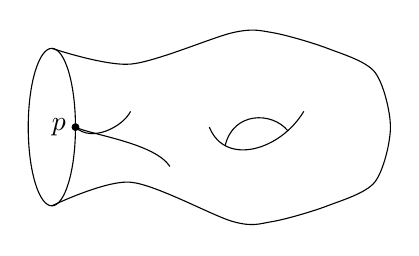
\begin{tikzpicture}
  %\draw plot [smooth cycle] coordinates {(0, 0) (-0.4, -0.5) (-0.5, -1) (-0.4, -1.7) (-0.2, -2) (0, -1.9) (0.4, -1.5) (0.5, -1.1) (0.55, -0.7) (0.4, -0.3)};
  \draw plot [smooth] coordinates {(0, 0) (1, -0.2) (2.3, 0.2) (2.8, 0.2) (3.5, 0) (4.1, -0.3) (4.3, -1) (4.1, -1.7) (3.5, -2) (2.8, -2.2) (2.3, -2.2) (1, -1.7) (0, -2)};
  \draw (0, -1) ellipse(0.3 and 1);
  \draw (2, -1)..controls(2.2, -1.5)and(2.9, -1.3)..(3.2, -0.8);
  \draw (2.2, -1.24)..controls(2.3, -0.8)and(2.8, -0.8)..(3, -1.05);
  \filldraw (0.3, -1) circle (1.2pt) node [left] {$p$};
  \draw (0.3, -1)..controls(0.5, -1.2)and(0.9, -1)..(1, -0.8);
  \draw (0.3, -1)..controls(0.5, -1.1)and(1.3, -1.2)..(1.5, -1.5);
\end{tikzpicture}
\end{wrapfigure}

Dla rozmaitości $M$ z brzegiem i $p\in \partial M$ dopuszczamy dodatkowo krzywe gładkie $c:[t_0, b)\to M $ oraz $c:(a, t_0[\to M$ takie, że $c(t_0)=p$ oraz pary $(c, t_0)$ jako elementy $C_pM$. Inaczej dla niektórych "kierunków" wektorów nie istniałyby odpowiednie krzywe reprezentujące te wektory. Styczność na $T_pM$ określa się potem w sposób analogiczny jak dla rozmaitości bez brzegu.
\medskip

Wektory styczne do $M=\R^n$ (lub $U\subseteq \R^n$) w punkcie $p$ odpowiadające wektorom bazowym $e_1=(1,0,0,...,0), e_2=(0, 1, 0, ..., 0) ,...,e_n=(0,0,0,...,1)$ oznaczamy przez $\frac{\partial}{\partial x_1}(p),\frac{\partial}{\partial x_2}(p),...,\frac{\partial}{\partial x_n}(p)$. Tworzą one bazę $T_p\R^n$ ($T_pU$), zaś dowolny wektor z $T_p\R^n$ ($T_pU$) ma postać $\sum_{i=1}^na_i\frac{\partial}{\partial x_i}(p)$.
\marginpar[]{Sens wprowadzenia takiego oznaczenia stanie się jasny później, gdy wektory utożsamimy z tzw. derywacjami}[0cm]

Analogicznie, dla dowolnej rozmaitości $M$ i $p\in M$ oraz mapy $\phi$ wokół $p$ przeciwobraz przez $\phi_p^*:T_pM\to\R^n$ wersorów $e_1,...,e_n$ oznaczamy:
$$\color{green}(\phi_p^*)^{-1}(e_i)=\frac{\partial}{\partial\phi_i}(p).$$
Elementy te tworzą bazę $T_pM$ i dowolny wektor z $T_pM$ ma postać $\sum a_i\frac{\partial}{\partial\phi_i}(p)$.

\begin{figure}[ht]
  \begin{illustration}
    \draw(2, 2)rectangle(4, 4) node [above] {$\R^n$};
    \draw[->] (3, 1.8)--(3, 4.2);
    \draw[->] (1.8, 3)--(4.2, 3);
    \draw[->, very thick] (3, 3)--(3, 3.7) node [left] {$e_2$};
    \draw[->, very thick] (3, 3)--(3.7, 3) node [below] {$e_1$};

    \draw(-2, 0) arc (180:270:1);
    \draw(-1, 0) arc (220:280:1);
    \draw(-0.9, -0.1) arc (110:30:0.6);
    \draw(-1, -1) arc (90:45:2);
    \draw(0.41, -1.578) arc (220:300:1.5);
    \draw(2.3,-1.915) arc (300:400:1.2);
    \draw(2.626, -0.104) arc (50:90:3);

    \draw plot [smooth, tension=1] coordinates {(0.7, 0.6) (0, 0.7)  (-1.4,1) (-2, 0)};

    \draw plot[domain=0:350,smooth cycle, xshift=1.5cm, yshift=-0.8cm] (\x:0.5+rnd*0.2);
    \node at (0.8, -1.3) {$U$};

    \draw (0.5, -1.8)--(3, -1.5)--(2.5, 0.2)--(0, -0.1) node [above] {$T_pM$} -- cycle;
    \draw[very thick, ->] (1.5, -0.8)--(1.05, 0.3);
    \draw[very thick, ->] (1.5, -0.8)--(3, -0.55);
    
    \draw[<-] (4, -2)--(4, -4);
    \draw[->] (3, -3)--(5, -3) node [above] {$\R^n$};


    \draw plot[domain=0:350,smooth cycle, xshift=4cm, yshift=-3cm] (\x:0.4+rnd*0.2);

    \draw[->] (2.3, -1)..controls(3, -1)and(3.5, -1.8)..(3.7, -2.5) node [midway, above] {$\phi$};

    \draw[->] (2.7, 0)..controls(3, -0.1)and(4, 0.2)..(3.5, 1.8) node [midway, right] {$\phi_p^*$};
    
    \draw (1.1, -0.1)..controls(0.5, -0.2)and(0, 0.5)..(-0.5, 1.7) node [above] {$\frac{\partial}{\partial\phi_2}(p)$};
    \draw (2.9, -0.6)..controls(3.5, -0.5)and(4.5, -0.3)..(5, 0.5) node [above] {$\frac{\partial}{\partial\phi_1}(p)$};
  \end{illustration}
\end{figure}

Dla gładkiej $c:(a, b)\to M$ \acc[b]{wektor styczny} do $c$ w $t\in(a, b)$ to 
$$c'(t):=[c, t]=[(\phi\circ c)'(t)]=\sum_i(\phi\circ c)'_i(t)\frac{\partial}{\partial\phi_i}(c(t)),$$ gdzie $(U, \phi)$ jest mapą wokół $c(t)$.

\subsection{Różniczka}

Rozważmy funkcję gładką $f:M\to N$ i $p\in M,f(p)=q\in N$. Dla krzywej zbalansowanej $(c, t_0)\in C_pM$ mamy $(f\circ c, t_0)\in C_qN$.

\begin{lemma}[krzywe styczne po przejściu przez f:M->N są nadal styczne] \label{styczne po przejsciach}
  Jeżeli $(c_1, t_1),(c_2, t_2)\in C_pM$ są styczne, to $(f\circ c_1, t_1),(f\circ c_2, t_2)\in C_qN$ też są styczne
\end{lemma}

\begin{proof}
  Niech $\phi$ będzie mapą wokół $p$, $\phi:U\to\R^m$, zaś $\psi$ mapą wokół $q$,

  $\psi:W\to\R^n$
  \begin{align*}(\psi\circ f\circ c_1)'(t_1)&=[(\psi\circ f\circ\phi^{-1})\circ(\phi\circ c_1)]'(t_1)=D_{\phi(p)}(\psi\circ f\circ \phi^{-1})\cdot[(\phi\circ c_1)'(t_1)]=\\
  &=D_{\phi(p)}(\psi\circ f\circ\phi^{-1})\cdot[(\phi\circ c_2)'(t_2)]=[(\psi\circ f\circ\phi^{-1})\circ(\phi\circ c_2)]'(t_2)=\\
  &=(\psi\circ f\circ c_2)'(t_2)\end{align*}
  Zatem krzywe $(f\circ c_1, t_1)$ i $(f\circ c_2, t_2)$ są styczne.
\end{proof}

\begin{definition}[różniczka] \important{Różniczką} $f$ w punkcie $p$ nazywamy odwzorowanie $df_p:T_pM\to T_{f(p)}N$ określone przez $df_p([c, t_0])=[f\circ c, t_0]$.
\end{definition}

Odwzorowanie różniczkowe jest dobrze określone na mocy Lematu \ref{styczne po przejsciach}.

\begin{lemma}[df jest odwzorowaniem liniowym]
  $df_p:T_pM\to T_{f(p)}N$ jest odwzorowaniem liniowym.
\end{lemma}

\begin{proof}
  Wystarczy sprawdzić, że odwzorowanie

  \begin{center}\begin{tikzcd}
    \R^m\arrow[r, "\lambda_{\phi,p}"] & T_pM \arrow[r, "df_p"] & T_{f(p)}N\arrow[r, "\psi_{f(p)}^*"] & \R^n
  \end{tikzcd}\end{center}
  jest liniowe (analogicznie jak przy dowodzie \ref{przestrzen styczna jest wektorowa}). 
  \begin{align*}
    \psi_{f(p)}\circ df_p\circ\lambda_{\phi, p}(v)&=\psi_{f(p)}^*\circ df_p([c_v, 0])=\psi_{f(p)}^*([f\circ c_v, 0])=\\
                                                  &=(\psi\circ f\circ c_v)'(0)=[(\psi\circ f\circ \phi^{-1})\circ(\phi\circ c_v)]'(0)=\\
                                                  &=D_{\phi(p)}(\psi\circ f\circ\phi^{-1})\cdot[(\phi\circ c_v)'(0)]=\\
                                                  &=D_{\phi(p)}(\psi\circ f\circ \phi^{-1})[v]
  \end{align*}
  jest to przekształcenie zadane macierzą, a więc liniowe.
\end{proof}

Dla gładkiej funkcji $f:M\to N$ odwzorowanie $df_p:T_pM\to T_{f(p)}N$ wyznaczyliśmy w mapach $\phi$ wokół $p$ i $\psi$ wokół $f(p)$ jako
$$\psi_{f(p)}^*df_p\lambda_{\phi, p}(p)=D_{\phi(p)}(\psi f\phi^{-1})(v).$$
Stąd, odwzorowanie $df_p$ w bazach $\{\frac{\partial}{\partial\phi_i}(p)\}$ w $T_pM$ i $\{\frac{\partial}{\partial\psi_j}(p)\}$ w $T_{f(p)}N$ zapisuje się macierzą
$$D_{\phi(p)}(\psi f\phi^{-1})=\left(\frac{\partial(\psi f\phi^{-1})_i}{\partial x_j}(\phi(p))\right)_{ij}$$
$$df_p\left[\sum a_i\frac{\partial}{\partial\phi_i}(p)\right]=\sum_i\left[\sum_j\frac{\partial(\psi f\phi^{-1})}{\partial x_j}(\phi(p))\cdot a_j\right]\frac{\partial}{\partial\psi_i}(f(p)) $$

\textbf{Przykłady:}
\phantomsection\label{phi z gwiazdka to d phi}
\begin{itemize}
  \item Niech $\phi:U\to\R^n$ będzie mapą wokół $p\in M$. Możemy ją potraktować jako gładkie odwzorowanie między dwiema rozmaitościami. Wówczas różniczka $d\phi_p:\underset{{\scriptstyle =T_pM}}{T_pU}\to T_{\phi(p)}\R^n$ jest wówna odwzorowaniu "mapowemu" $\phi_p^*:T_pM\to\R^n$.

    \begin{proof}
      Niech $[c, t_0]\in T_pM$, wtedy
      $$d\phi_p([c, t_0])=[\phi\circ c, t_0]\in T_{\phi(p)}\R^n$$
      Mapę $(id_{\R^n})^*_{\phi(p)}:T_{\phi(p)}\R^n\to \R^n$ \hyperref[mapa na T_pR]{kanonicznie utożsamiliśmy} z $id_{\R^n}$, stąd też
      $$d\phi_p([c, t_0])=(id_{\R^n}\circ\phi\circ c)'(t_0)=(\phi\circ c)'(t_0),$$
      a z kolei
      $$\phi_p^*([c, t_0])=(\phi\circ c)'(t_0)\in\R^n$$
      z definicji tego odwzorowania.
    \end{proof}
  \item Dla gładkiej krzywej $c:(a, b)\to M$ oraz $t_0\in (a, b)$, różniczka $dc_{t_0}:T_{t_0}(a, b)\to T_{c(t_0)}M$ jest jedynym przekształceniem liniowym, które wersor z $\R\cong T_{t_0}(a, b)$ przekształca na wersor $[c, t_0]=c'(t_0)\in T_{c(t_0)}M$.
  \item Rozważmy gładką funkcję $f:M\to \R$ i $p\in M$. Różniczka $df_p:T_pM\to T_{f(p)}\R\cong \R$ jest funkcjonałem liniowym na $T_pM$. 
\end{itemize}

\begin{definition}[pochodna kierunkowa]
Dla funkcji $f:M\to\R$ możemy wybrać wektor styczny $X=[c, t_0]\in T_pM$ i zdefiniować \important{pochodną kierunkową} funkcji $f$ w kierunku wektora $X$: 
$$\color{blue}Xf=df_p(X)=df_p([c, t_0])=(f\circ c)'(t_0).$$
\end{definition}

Pochodna kierunkowa ma następujące własności:
\begin{itemize}
  \item $X(f+g)=Xf+Xg$
  \item $X(f\cdot g)=g(p)\cdot Xf+f(p)\cdot Xg$ (\acc[i]{reguła Leibniza})
    \begin{proof}
      \begin{align*}
        X(f\cdot g)&=[(f\cdot g)\circ c]'(t_0)=[(f\circ c)\cdot(g\circ c)]'(t_0)=\\
                            &=(f\circ c)'(t_0)\cdot(g\circ c)(t_0)+(f\circ c)(t_0)\cdot(g\circ c)'(t_0)=\\
                            &=Xf\cdot g(p)+f(p)\cdot Xg
      \end{align*}
    \end{proof}
  \item dla $a\in \R$ $(aX)f=a(Xf)$
  \item jeśli $X, Y\in T_pM$, to $(X+Y)f=Xf+Yf$
    \begin{proof}
      $$(X+Y)f=df_p(X+Y)=df_p(X)+df_p(Y)=Xf+Yf$$
    \end{proof}
\end{itemize}

\textbf{Przykłady:}
\begin{itemize}
  \item \marginpar{Stąd oznaczenie $\frac{\partial}{\partial x_i}(p)$, które ma charakter operatorowy związany z działaniem tego wektora na funkcjach $f_n$}Jeśli $X=\frac{\partial}{\partial x_i}(p)\in T_p\R^n$ i mamy gładką funkcję $f:\R^n\to\R$, to wówczas $Xf=\frac{\partial f}{\partial x_i}(p)$. 
  \item \marginpar{$\frac{\partial f}{\partial\phi_i}$ jest to $i$-ta pochodna cząstkowa $f$ w mapie $\phi$ w punkcie $p$}Jeśli $X=\frac{\partial}{\partial\phi_i}(p)\in T_pM$ i $f:M\to\R$ jest funkcją gładką, to oznaczamy 
    $$Xf=\frac{\partial(f\phi^{-1})}{\partial x_i}(\phi(p)=:\frac{\partial f}{\partial \phi_i}(p)$$
  \item Podobnie jak wyżej, jeśli $X=\sum a_i\frac{\partial}{\partial \phi_i}(p)$, to
    $$Xf=\sum a_i\frac{\partial f}{\partial\phi_i}(p)=\sum a_i\frac{\partial f\circ\phi^{-1}}{\partial x_i}(\phi(p))$$
\end{itemize}

\subsection{Wiązka styczna}

\begin{definition}[wiązka styczna]
  Wiązka styczna to rozłączna suma przestrzeni stycznych we wszystkich punktach rozmaitości $M$:
  $$\color{blue}TM=\bigsqcup_{p\in M}T_pM$$
\end{definition}

Chcemy teraz opisać na $TM$ strukturę rozmaitości gładkiej. Rozważymy w tym celu rzutowanie
$$\pi:TM\to M$$
$$\pi(v)=p,\quad v\in T_pM,$$
które wektorowi przyporządkowuje jego punkt zaczepienia.

\begin{lemma}[wiązka styczna jest $2n$-rozmaitością]
  Niech $M$ będzie rozmaitością $n$-wymiarową $M$ klasy $C^k$. Wówczas na wiązce stycznej $TM$ istnieje naturalna struktura $2n$-wymiarowej rozmaitości klasy $C^{k-1}$, dla której rzutowanie $\pi$ jest $C^{k-1}$-różniczkowalne.

  Jeśli $M$ jest rozmaitością gładką ($C^\infty$), to $\pi$ również takie jest.
\end{lemma}

\begin{proof}

  Strukturę rozmaitości zadamy za pomocą samych map, nie definiując właściwej topologii na $TM$.

  \begin{figure}[ht]
    \centering\scalebox{0.8}{
      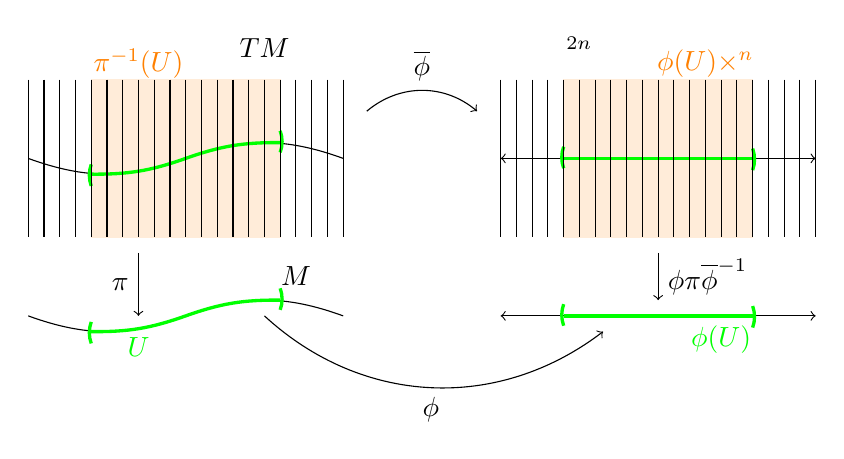
\begin{tikzpicture}
        \filldraw[orange!15] (0.8, 1) rectangle (3.2, -1);
        \filldraw[orange!15] (6.8, 1) rectangle (9.2, -1);

        %\draw[step=0.2,orange,thin] (-1,4) grid (10,-4);
        \path (0, -2) edge [bend right=20] (2, -2);
        \path (2, -2) edge [bend left=20] (4, -2);
        \path[green, very thick] (0.8, -2.2) edge [bend right=10] (2, -2);
        \path[green, very thick] (2, -2) edge [bend left=10] (3.2, -1.8);
        \draw[green, very thick] (0.8, -2.35) arc (200:160:0.4);
        \draw[green, very thick] (3.2, -1.65) arc (20:-20:0.4);

        \path (0, 0) edge [bend right=20] (2, 0);
        \path (2, 0) edge [bend left=20] (4, 0);
        \path[green, very thick] (0.8, -0.2) edge [bend right=10] (2, 0);
        \path[green, very thick] (2, 0) edge [bend left=10] (3.2, 0.2);
        \draw[green, very thick] (0.8, -0.35) arc (200:160:0.4);
        \draw[green, very thick] (3.2, 0.35) arc (20:-20:0.4);

        \draw[<->] (6, 0)--(10, 0);
        \draw[green, very thick] (6.8, 0)--(9.2, 0);
        \draw[green, very thick] (6.8, -0.125) arc (200:160:0.4);
        \draw[green, very thick] (9.2, 0.125) arc (20:-20:0.4);
        
        \draw[<->] (6, -2)--(10, -2);
        \draw[green, very thick] (6.8, -2)--(9.2, -2);
        \draw[green, very thick] (6.8, -2.125) arc (200:160:0.4);
        \draw[green, very thick] (9.2, -1.875) arc (20:-20:0.4);

        \foreach \x in {0,...,20}
          \draw (0.2*\x, 1)--(0.2*\x, -1);

        \foreach \x in {0,...,20}
          \draw (6+0.2*\x, 1)--(6+0.2*\x, -1);

        \node at (3, 1.4) {$TM$};
        \node at (3.4, -1.5) {$M$};
        \node at (1.4, -2.4) {$\color{green}U$};
        \node at (1.4, 1.2) {$\color{orange}\pi^{-1}(U)$};

        \node at (7, 1.4) {$\R^{2n}$};
        \node at (8.6, 1.2) {$\color{orange}\phi(U)\times\R^n$};
        \node at (8.8, -2.3) {$\color{green}\phi(U)$};

        \path[->] (4.3, 0.6) edge [bend left=40] node [midway, above] {$\overline{\phi}$} (5.7, 0.6);
        \draw[->] (1.4, -1.2)--(1.4, -2) node [midway, left] {$\pi$};
        \path[->] (3, -2) edge [bend right=40] node [midway, below] {$\phi$} (7.3, -2.2);
        \draw[->] (8, -1.2)--(8, -1.8) node [midway, right] {$\phi\pi\overline{\phi}^{-1}$};
    \end{tikzpicture}}
  \end{figure}
  Niech $(U,\phi)$ będzie mapą na $M$. Rozważmy zbiór 
  $$TU=\pi^{-1}(U)=\bigcup_{p\in U}T_pM\subseteq TM$$
  oraz odwzorowanie
  $$\overline{\phi}:TU\to\R^{2n}=\R^n\times\R^n$$
\marginpar{$\phi_p^*([c, t_0])=(\phi\circ c)'(t_0)$}
\hyperref[phi z gwiazdka]{%
  \texorpdfstring{%
    $$\overline{\phi}(v)=(\;\phi(\pi(v)),\;{\color{blue}\phi^*_{\pi(v)}(v)}\;)=(\;\phi(p),\;\phi_p^*(v)\;)\quad v\in T_pM.$$%
  }%
}%
  $\overline{\phi}$ jest różniczkowalne jako produkt kartezjański dwóch różniczkowalnych odwzorowań, a jego obraz to $\phi(v)\times\R^n$.

  Sprawdźmy teraz zgodność tak zadanego atlasu. Niech $(U,\phi)$ i $(V,\psi)$ będą mapami na $M$, a $(TU, \overline{\phi}),(TV,\overline{\psi})$ odpowiadającymi im mapami na $TM$. Spójrzmy na odwzorowania przejścia:
  $$\overline{\psi}\circ\overline{\phi}^{-1}:\phi(U\cap V)\times\R^n\to\psi(U\cap V)\times\R^n$$
  \begin{align*}
    \overline{\psi}\overline{\phi}^{-1}(x,w)&=(\;\psi\pi[\phi\pi]^{-1}(x),\;\psi^*_{\phi^{-1}(x)}[\phi^*_{\phi^{-1}(x)}]^{-1}(w)\;)=\\
                                            &=(\;\psi\phi^{-1}(x),\;D_x(\psi\phi^{-1})(w)\;)
  \end{align*}
  Jest to odwzorowanie różniczkowalne klasy $C^{k-1}$ jako produkt odwzorowania klasy $C^k$ i $C^{k-1}$.

  Pozostaje sprawdzić różniczkowalność odwzorowania $\pi$. Wyrazimy je w mapach $(U,\phi)$ na $M$ oraz $(TU,\overline{\phi})$ na $TM$. Niech $p\in U$ oraz $v\in T_pU$, wtedy:
  \begin{align*}
    \phi\pi\overline{\phi}^{-1}(\phi(p),\phi_p^*(v))=\phi\pi(v)=\phi(p)
  \end{align*}
  więc $\pi$ jest w tych mapach rzutowaniem na pierwszą składową $\R^{n}$, więc jest gładkie

\end{proof}

\begin{definition}
  Dla $f:M\to N$ \important{odwzorowaniem stycznym} $df:TM\to TN$ nazywamy odwzorowanie
  $$df(v)=df_{\pi(v)}(v)\in T_{f(\pi(v))}N\subseteq TN$$
\end{definition}

\begin{lemma}Dla gładkiego $f$ również $df$ jest gładkie.
\end{lemma}

\begin{proof}
  Weźmy $v\in T_pM$ i niech $(U,\phi)$ będzie mapą wokół $p$. Oznaczmy wówczas $q=f(p)$ i niech $(V, \psi)$ będzie mapą wokół $q$. Wyrazimy $df$ w mapach $(TU,\overline{\phi})$ i $(TV,\overline{\psi})$.

  \begin{center}
    \begin{tikzcd}
      \R^{2m}\arrow[r, "\overline{\phi}^{-1}"] & TU\arrow[r, "df"] & TV\arrow[r, "\overline{\psi}"] & \R^{2n}
    \end{tikzcd}
  \end{center}

  \begin{align*}
    \overline{\psi}df\overline{\phi}^{-1}(x, w)&=(\;\psi f\phi^{-1}(x),\;\psi^*_{f\phi^{-1}(x)}df_{\phi^{-1}(x)}[\phi^*_{\phi^{-1}(x)}]^{-1}(w)\;)\overset{1}{=}\\
                                               &=(\;\psi f\phi^{-1}(x),\; d\psi_{f\phi^{-1}(x)}df_{\phi^{-1}(x)}(d\phi_{\phi^{-1}(x)})^{-1}(x)\;)\overset{2}{=}\\
                                               &=(\;\psi f\phi^{-1}(x),\; d\psi_{f\phi^{-1}(x)}df_{\phi^{-1}(x)}d\phi^{-1}_x(w)\;)\overset{3}{=}\\
                                               &=(\;\psi f\phi^{-1}(x),\;d(\psi f\phi^{-1})_x(w)\;)=\\
                                               &=(\;\psi f\phi^{-1}(x),\;D_x(\psi f\phi^{-1})(x)\;)
  \end{align*}
  Równość $1$ wynika z utożsamienia $d\phi_p=\phi_p^*$ (\hyperref[phi z gwiazdka to d phi]{uzasadnione tutaj}). Równość $2$ to ogólny fakt, że jeśli $f$ jest dyfeomorfizmem, to $(df_p)^{-1}=df^{-1}_{f(p)}$, natomiast równość $3$ pojawia się na liście ćwiczeń: 
  $$d(f\circ g)_p=df_{g(p)}\circ dg_p.$$
\end{proof}

\begin{remark}
  Różniczka $df_p$ jak w lemacie wyżej zapisuje się w bazach $\{\frac{\partial}{\partial\phi_i}(p)\}$ w $T_pM$ oraz $\{\frac{\partial}{\partial\psi_j}(q)\}$ w $T_qN$ przy pomocy macierzy:
  $$D_{\phi(p)}(\psi f\phi^{-1})=\left(\frac{\partial(\psi f\phi^{-1})}{\partial x_j}(\phi(p))\right)_{i,j}.$$
  To znaczy ma postać:
  $$df_p\left[\sum a_i\frac{\partial}{\partial\phi_i}(p)\right]=\sum_i\left[\sum_j\frac{\partial(\psi f\phi^{-1})_i}{\partial x_j}(\phi(p))\cdot a_j\right]\frac{\partial}{\partial\psi_i}(q)$$
\end{remark}

\begin{example}
\item Dla otwartego $U\subseteq\R^n$, wiązka styczna $TU$ do $U$ utożsamia się z $U\times\R^n$ poprzez
  $$\sum_{i\leq n}a_i\frac{\partial}{\partial x_i}(p)\mapsto (\;p,\;a_1,...,a_n\;)$$
\end{example}

  Niech $f:M\to N$ i $g:N\to P$ będą odwzorowaniami gładkimi, wtedy:
  \begin{itemize}
\marginpar{Dowód tych właności jest ćwiczeniem}
    \item $d(g\circ f)=dg\circ df$
    \item $d(id_M)=id_{TM}$
    \item jeśli $f$ jest dyfeomorfizmem, to również $df$ jest dyfeomorfizmem oraz $(df)^{-1}=df^{-1}$
  \end{itemize}

\newpage
%
\section{Pola wektorowe}

\begin{definition}
  Niech $M$ będzie gładką rozmaitością. Gładką funkcję $X:M\to TM$ taką, że dla każdego $p\in M$ $X(p)\in T_pM\subseteq TM$ nazywamy \important{gładkim polem wektorowym} na $M$.

  Równoważnie możemy postawić warunek, że $\pi\circ X=id_M$.
\end{definition}

Często zamiast $X(p)$ piszemy krócej $X_p$, co oznacza wektor pola w punkcie $p$. \marginpar{Uogólnienie pól wektorowych pojawiających się w kontekście równań różniczkowych.}Pozwala to również uniknąć konfliktu notacji z pochodną kierunkową funkcji $f$ wzdłuż wektora $X$ ($Xf$).
  

\begin{center}
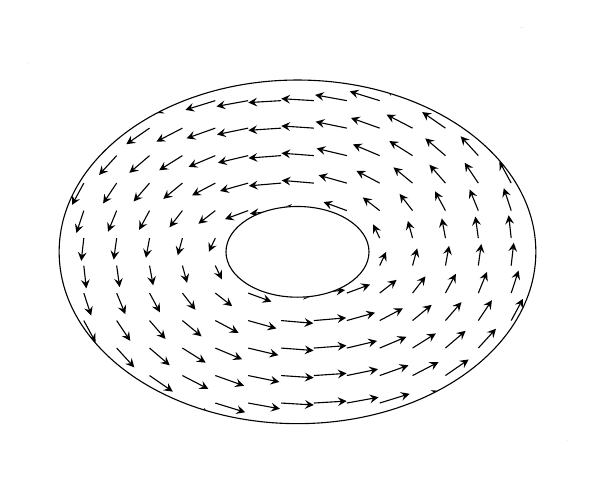
\begin{tikzpicture}[even odd rule]
%  \draw[rounded corners=35pt] (6.5,-1.8)--(2,-2)--(0,0) -- (2,2)--(4.2,1.4)--cycle;
%  \draw (3.5, 0.2) arc (-20:-130:0.9 and 0.7);
%  \draw (2.3, -0.15) arc (180:40:0.6 and 0.3);
%
%  \draw[thick, ->] (1.1, 0)--(1.4, 0.6);
%  \draw[thick, ->] (1.5, -0.6)--(1.6, 0.2);
%  \draw[thick, ->] (1.2, 0.8)--(2, 1.4);
%  \draw[thick, ->]  

\begin{axis}[%
  view     = {0}{90}, % for a view 'from above'
  domain   = -3:3,
  y domain = -3:3,
  %xtick    = {-3,...,3},
  %ytick    = {-3,...,3},
  axis line style={draw=none},
  ticks=none
  %tick style={draw=none}
]
\addplot3[
        quiver = {
            u = {-y/sqrt(x^2+y^2)},
            v = {x/sqrt(x^2+y^2+3)},
            scale arrows = 0.4,
        },
        -stealth,
        domain = -3:3,
        domain y = -3:3,
        samples=16
    ] {0};
%\addplot3[blue, quiver={u=8*x, v=2*y, scale arrows=0.05}, samples=16, -latex] (x,y,0);

  %\fill[clip, overlay=false, fill=white, color=white, fill opacity=0.5] (-4, 3.5) rectangle (5, -3.5) ellipse (0, 0) (1 and 0.5);

  \fill[preaction={clip}, fill=white] (-4,-3.5) rectangle (4,3.5) (0,0) ellipse (2.9 and 2.5);
  \draw (0,0) ellipse (2.9 and 2.5);
  \filldraw[white] (0,0) ellipse (0.84 and 0.66);
  \draw (0,0) ellipse (0.87 and 0.66);
 
\end{axis}
\end{tikzpicture}
\end{center}

Wyraźmy pole wektorowe $X:M\to TM$ w mapach $(U,\phi)$ na $M$ oraz $(TU,\overline{\phi})$ na $TM$. Niech $a_i:\phi(U)\to\R$ będą gładkimi funkcjami rzeczywistymi (nazwiemy je \acc[i]{współrzędnymi $X$} w mapach $\phi$ i $\overline{\phi}$) takimi, że
$$\overline{\phi}X\phi^{-1}(x)=(\;x,\;a_1(x),...,a_n(x)\;)=(\;x,\;\sum a_i(x)e_i\;),$$
gdzie $e_i$ to baza standardowa $\R^n$. Zgodnie z oznaczeniem z poprzedniego rozdziału $\frac{\partial}{\partial \phi_i}(p)=(\phi^*_p)^{-1}(e_i)$ mamy
$$X(p)=\sum a_i(\phi(p))\cdot\frac{\partial}{\partial\phi_i}(p).$$
Jeśli teraz oznaczymy $b_i=a_\circ\phi:U\to\R$, to wówczas
$$X(p)=\sum b_i(p)\cdot\frac{\partial}{\partial\phi_i}(p).$$

\begin{fact}
  Pole $X:M\to TM$ jest gładkim polem wektorowym na $M$ $\iff$ w mapie $(U,\phi)$ na $M$ i odpowiadającej jej mapie $(TU,\overline{\phi})$ na $TM$ wyraża się jako
  $$X(p)=\sum b_i(p)\cdot\frac{\partial}{\partial\phi_i}(p)$$
  dla pewnych gładkich $b_i:U\to\R$.
\end{fact}

\begin{proof}
  Bezpośrednio z przestawienia $X$ w mapach $(U,\phi)$ i $(TU,\overline{\phi})$ jak wyżej.
\end{proof}

Pole wektorowe na otwartym $U\subseteq\R^n$ ma postać
$$X(x)=\sum_{i\leq n}a_i(x)\cdot\frac{\partial}{\partial x_i}(x)$$
dla pewnych gładkich funkcji $a_i:U\to\R$. Z tego powodu będziemy pisać
$$X(x)=[a_1(x),...,a_n(x)]\in \R^n\cong T_xU.$$
Zjawiska lokalne dla pól na rozmaitościach będziemy wyrażać za pośrednictwem map za pomocą pól na otwartych podzbiorach $\R^n$.

\begin{conclusion}\label{wniosek 5:3}
  Suma dwóch gładkich pól wektorowych
  $$(X+Y)(p):=X(p)+Y(p)$$
  jest gładkim polem wektorowym.

  Iloczyn gładkiej funkcji $f:M\to\R$ oraz gładkiego pola $X$
  $$(f\cdot X)(p):=f(p)\cdot X(p)$$
  jest gładkim polem wektorowym
\end{conclusion}

Rodzinę wszystkich gładkich pól wektorowych na $M$ będziemy oznaczać przez $C^\infty(TM)$ lub $\color{blue}\mathfrak{X}(M)$. W algebraicznym rozumienia jest to moduł nad pierścieniem $C^\infty(M)$ gładkich funkcji rzeczywistych na $M$ (patrz wniosek \ref{wniosek 5:3}).

\subsection{Definiowanie pola wektorowego za pomocą rozkładów jedności}

Niech $M$ będzie rozmaitością z niepustym brzegiem $\partial M$. 

\begin{definition}
  Mówimy, że wektor $Y\in T_pM$, gdzie $p\in\partial M$, jest \important{skierowany do wewnątrz} $M$, jeśli w pewnej mapie $\phi:U_p\to H^n$ wyraża się przez
  $$Y=\sum_{i\leq n}a_i\cdot\frac{\partial}{\partial\phi_i}(p),\quad a_n>0$$
\end{definition}

\begin{fact}
  Jeśli wektor o początku $p$ jest skierowany do wewnątrz w jednej mapie, to jest tak w każdej innej mapie wokół $p$. Ponadto, suma wektorów skierowanych do wewnątrz jest wektorem skierowanym do wewnątrz.
\end{fact}

\begin{proof}
  Niech $Y$ będzie wektorem skierowanym do wewnątrz w mapie $(U,\phi)$. Niech $(V, \psi)$ będzie inną mapą wokół $p$. Wiemy, że
  $$Y=\sum a_i\cdot\frac{\partial}{\partial\phi_i}(p)$$
  i $a_n>0$. Chcemy teraz sprawdzić, co się dzieje w indeksie $n$, gdy przedstawimy ten wektor jako kombinację liniową $\frac{\partial}{\partial\psi_i}(p)$. Popatrzmy na zamianę baz:
  \begin{align*}
    \frac{\partial}{\partial\phi_n}(p)&=(\phi^*_p)^{-1}(e_n)=\\
        &=(\psi_p^*)^{-1}[\psi_p^*(\phi_p^*)^{-1}](e_n)=\\
        &=(\psi_p^*)^{-1}d\psi_p d(\phi)^{-1}_{\phi(p)}(e_n)=\\
        &=(\psi_p^*)^{-1}[d(\psi\phi^{-1})_{\phi(p)}(e_n)]
  \end{align*}
  Wiemy, że $\psi\phi^{-1}:\R^n\to\R^n$ jest funkcją rzeczywistą, czyli 
  $$d(\psi\phi^{-1})_{\phi(p)}=D_{\phi(p)}(\psi\phi^{-1})$$
  jest jej pochodną. Dodatkowo, wiemy, że $\psi\phi^{-1}$ jest bijekcją, więc na pewno $D_{\phi(p)}(\psi\phi^{-1})(e_n)$ nie może się zerować. Zarówno $\psi$ jak i $\phi$ są mapami wokół brzegu $\partial M$, czyli tak naprawdę:
  $$\psi\phi^{-1}:H^n\to H^n$$
  W takim razie, $D_{\phi(p)}(\psi\phi^{-1})(e_n)\in \{(x_1,...,x_n)\in\R^n\;:\;x_n>0\}$.% i 
  %$$a_n\cdot\frac{\partial}{\partial\phi_n}(p)=\underbrace{a_n\cdot D_{\phi(p)}(\phi\psi^{-1})(e_n)}_{>0}\cdot\frac{\partial}{\partial\psi_n}$$

  \begin{center}
  \scalebox{0.6}{
  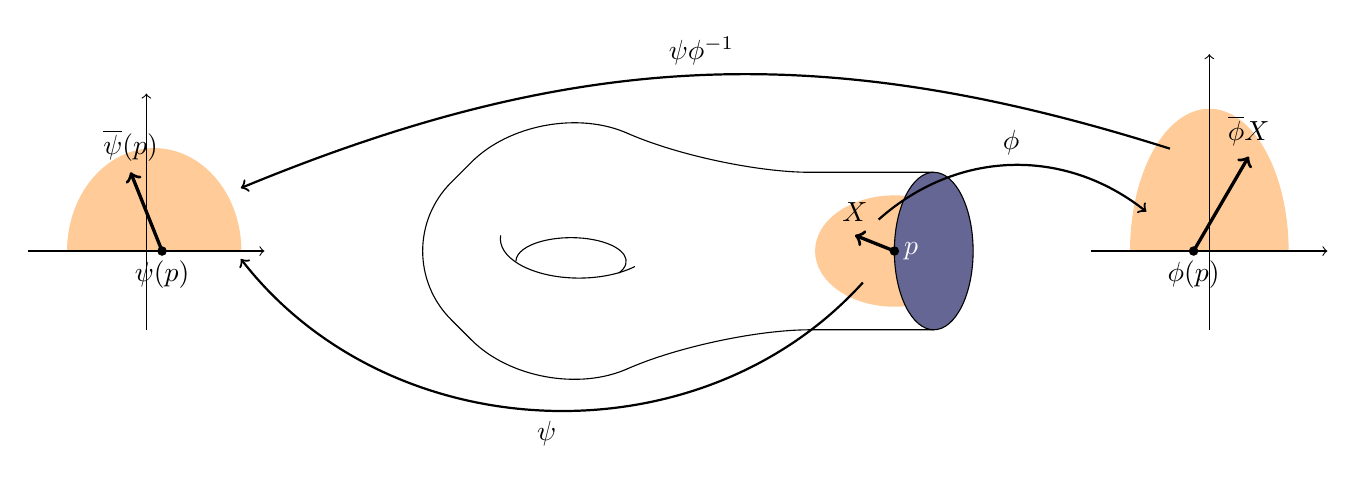
\begin{tikzpicture}
    \filldraw[orange!40] (6.5, 0) ellipse (1 and 0.7);
    \draw[->, very thick] (6.5, 0)--(6, 0.2);
      \draw[rounded corners=35pt](7,-1)--(4.2,-1)--(2,-2)--(0,0) -- (2,2)--(4.2,1)--(7,1);
      \draw (1.5,0.2) arc (175:315:1cm and 0.5cm);
      \draw (3,-0.28) arc (-30:180:0.7cm and 0.3cm);
      \filldraw[color=black, fill=blue!30!black!60](7.5,0) arc (0:360:0.5cm and 1cm);
      \filldraw (6.5, 0) circle (1.5pt) node [right] {$\color{white}p$};
      \node at (6, 0.5) {$X$};

      \filldraw[orange!40] (9.5, 0) arc (180:0:1 and 1.8);
      \draw[->] (9, 0)--(12, 0);
      \draw[->] (10.5, -1)--(10.5, 2.5);
      \filldraw(10.3, 0) circle (1.5pt) node [below] {$\phi(p)$};
      \draw[very thick, ->] (10.3, 0)--(11, 1.2) node [above] {$\overline{\phi}X$};
      
      \filldraw[orange!40] (-4, 0) arc (180:0:1.1 and 1.3);
      \draw[<-] (-1.5, 0)--(-4.5, 0);
      \draw[->] (-3, -1)--(-3, 2);
      \filldraw (-2.8, 0) circle (1.5pt) node [below] {$\psi(p)$};
      \draw[->, very thick] (-2.8, 0)--(-3.2, 1) node [above] {$\overline{\psi}(p)$};
      
      \path[->, thick] (6.3, 0.4) edge [bend left=40] node [midway, above] {$\phi$} (9.7, 0.5);
      \path[->, thick] (6.1, -0.4) edge [bend left=50] node [midway, below] {$\psi$} (-1.8, -0.1);
      \path[->, thick] (10, 1.3) edge [bend right=20] node [midway, above] {$\psi\phi^{-1}$} (-1.8, 0.8);
  \end{tikzpicture}}
  \end{center}
  

  %więc $Y$ zapisane w bazie $\frac{\partial}{\partial\psi_n}$ma ściśle dodatnią ostatnią współrzędną.

  Dla sumy wektorów $X+Y$ takich, że $X=\sum a_i\frac{\partial}{\partial\phi_i}(p)$ i $Y=\sum b_i\frac{\partial}{\partial\phi_i}(p)$, $a_n,b_n>0$, mamy
  $$X+Y=\sum(a_i+b_i)\frac{\partial}{\partial\phi_i}(p)$$
  więc $a_i+b_i>0$.
\end{proof}

\begin{definition}
  Pole wektorowe $X:M\to TM$ jest \important{skierowane do wewnątrz} $M$, jeśli dla każdego $p\in\partial M$ $X(p)$ jest skierowany do wewnątrz $M$.
\end{definition}

\begin{fact}\label{fakt:5.7}
  Na każdej rozmaitości gładkiej z brzegiem $M$ istnieje gładkie pole wektorowe $X$ skierowane do wewnątrz $M$.
\end{fact}

\begin{proof}
  Rozważmy rozkład jedności $\{f_i\}$ wpisany w pokrycie $M$ zbiorami mapowymi $U_\alpha$ i niech $supp(f_i)\subseteq U_{\alpha_i}$. Dla tych $U_\alpha$, które zahaczają o brzeg $\partial M$ określmy pola wektorowe
  $$X_\alpha:U_\alpha\to TU_\alpha\subseteq TM$$
  $$X_{\alpha}(p)=\frac{\partial}{\partial(\phi_\alpha)_n}(p).$$
  Dla pozostałych $U_\alpha$ określamy $X_\alpha$ dowolnie.

  \begin{figure}[h!]
    \begin{illustration}
      \filldraw[orange!20] (7.5, 0.25) arc (20:340:1 and 0.5);
      \draw[rounded corners=35pt](7,-1)--(4.2,-1)--(2,-2)--(0,0) -- (2,2)--(4.2,1)--(7,1);
      \draw (1.5,0.2) arc (175:315:1cm and 0.5cm);
      \draw (3,-0.28) arc (-30:180:0.7cm and 0.3cm);
      \filldraw[color=black, fill=blue!40!black!60] (7.5,0) arc (0:360:0.5cm and 1cm);

      \filldraw[orange!20] (8.5, 0) arc (180:0:1 and 1.3);
      \draw (8, 0)--(11, 0);
      \draw (9.5, 0)--(9.5, 1.5);

      \node at (6.5, 1.4) {$U_\alpha$};
      \node at (11, 0.5) {$\frac{\partial}{\partial x_n}$};
      \path (6.4, 1.2) edge [bend right=20] (6.3, 0.4);
      \path[->] (6, -0.2) edge [bend right=30] node [midway, below] {$\phi_\alpha$} (9, -0.3);
    \end{illustration}
  \end{figure}
  Zdefiniujmy teraz pole wektorowe:
  $$X=\sum_jf_jX_{\alpha_j},$$
  które jest lokalnie skończoną kombinacją gładkich pól skierowanych do wewnątrz i funkcji dodatnich. Jest to więc pole wektorowe skierowanie do wewnątrz.
\end{proof}

\subsection{Przenoszenie gładkich pól wektorowych przez dyfeomorfizmy}

Niech $f:M\to N$ będzie dyfeomorfizmem i niech $X\in\mathfrak{X}(M)$ będzie gładkim polem wektorowym na $M$. Poszczególne wektory $X_p$ pola $X$ przenoszone przez odwzorowanie styczne $df$ do $TN$ tworzą pola wektorowe na $N$ oznaczane przez $df(X)$ w ten sposób, że
$$\color{blue}df_p(X_p)=df(X)_{f(p)}.$$
Określamy pole wektorowe $df(X)$ na $N$ przez
$$df(X)_q:=df_{f^{-1}(q)}(X_{f^{-1}(q)})\in T_qN\subseteq N.$$
Powyższe określenia oznaczają, że pole $df(X)$, jako odwzorowanie $N\to TN$, jest złożeniem
$$\color{blue}df(X)=df\circ X\circ f^{-1}.$$
Jako złożenie odwzorowań gładkich, samo też jest odwzorowaniem gładkim.

\begin{definition}
  Gładkie pole wektorowe $df(X)$ określone jak wyżej jest nazywane \important{przeniesieniem} pola $X$ na $N$ przez dyfeomorfizm $f$.
\end{definition}

  Jeśli o dyfeomorfiźmie $f$ myślimy jako o sposobie utożsamienia rozmaitości $M$ i $N$, to o polu $df(X)$ na $N$ możemy myśleć jako o tym samym polu co pole $X$ na $M$ względem utożsamienia za pomocą $f$.

\begin{example}
  \item Wybierzmy pole $X\in\mathfrak{X}(M)$, takie, że dla mapy $(U,\phi)$ na $M$ mamy
    $$X(p)=\sum a_i(p)\cdot\frac{\partial}{\partial\phi_i}(p),\quad p\in U.$$
    Wówczas
    \begin{itemize}
      \item przeniesienie pola $X\restriction U$ na $\phi(U)$ przez dyfeomorfizm $\phi$ daje pole $d\phi(X)(u)=\sum a_i(\phi^{-1}(u))\cdot\frac{\partial}{\partial x_i}(x)$
      \item wyrażenie pola $X$ w mapach $(U,\phi)$ na $M$ oraz $(TU,\overline{\phi})$ na $TM$ daje
        $$\overline{\phi}X\phi^{-1}(x)=(\;x,\;a_1(\phi^{-1}(x)),...,a_n(\phi^{-1}(x))\;)$$
    \end{itemize}
    Oba te pola, a zwłaszcza pierwsze z nich, będziemy nazywać \acc[b]{wyrażeniem pola $X$}\marginpar{Dowód w lemacie \ref{lemat:5.10}} w mapie $(U,\phi)$. Ponadto zachodzi
    $$X(p)=[c,t_0]\iff d\phi(X)(\phi(p))=[\phi\circ c, t_0]$$
\end{example}

\subsection{Krzywe całkowe}

\begin{definition}
  Niech $M$ będzie rozmaitością bez brzegu. \important{Krzywą całkową} pola wektorowego $X\in\mathfrak{X}(M)$ to dowolna krzywa
  $$\gamma:(a,b)\to M$$
  taka, że dla każdego $t\in (a,b)$
  $$\gamma'(t)=[\gamma, t]=X(\gamma(t))$$
\end{definition}

\begin{lemma}\label{lemat:5.10}
  Niech $\gamma$ będzie krzywą całkową pola $X\in\mathfrak{X}(M)$ $\iff$ dla każdej mapy $(U,\phi)$ na $M$ krzywa $\phi\circ\gamma$ jest krzywą całkową pola $d\phi(X)\in\mathfrak{X}(\phi(U))$.
\end{lemma}

\begin{proof}$ $\newline

  $\implies$

  Jeśli $\gamma'(t)=[\gamma,t]=X_{\gamma(t)}$, to z definicji $d\phi$ mamy 
\reversemarginpar\marginpar{Dla przypomnienia: $df(X)_{f(p)}=df_p(X_p)$}
  $$(\phi\circ\gamma)'(t)=[\phi\circ\gamma,t]=d\phi_{\gamma(t)}([\gamma,t])=d\phi(X_{\gamma(t)})=d\phi(X)_{\phi\circ\gamma(t)}$$

  $\impliedby$

  Niech $(\phi\circ\gamma)'(t)=[\phi\circ\gamma,t]=d\phi(X)_{\phi\circ\gamma(t)}$. Wówczas
  \begin{align*}
    \gamma'(t)&=[\phi^{-1}(\phi\circ\gamma)]'(t)=d\phi^{-1}_{ \phi\circ\gamma(t)}[ (\phi\circ\gamma)'(t)]=\\
              &=d\phi_{\phi\circ\gamma(t)}[d\phi(X)_{\phi\circ\gamma(t)}]= \underbrace{d\phi^{-1}_{\phi\circ\gamma(t)}d\phi_{\gamma(t)}}_{id_{T_{\gamma(t)}M}}(X_{\gamma(t)})=X_{\gamma(t)}
  \end{align*}
\end{proof}

Krzywe całkowe mają \important{następujące własności}:
\begin{itemize}
  \item dla każdego $p\in M$ istnieje krzywa całkowa o początku w $p$ (twierdzenie \ref{istnienie krzywych calkowych})
  \item jeśli krzywe całkowe przecinają się, to są sobie równe (uwaga \ref{jednoznacznosc krzywych calkowych})
  \item krzywe całkowe pola na otoczeniu pewnego punktu $p\in M$ są gładko zależne (fakt \ref{gladka zaleznosc od punktu poczatkowego})
\end{itemize}
Które zostaną udowodnione niżej.

\begin{theorem}\label{istnienie krzywych calkowych} Dla \marginpar{Krzywe całkowe wyrażenia pola $X$ w mapie $(U,\phi)$ to wyrażenie krzywych całkowych pola $X$ w tej samej mapie.}każdego $p\in M$ istnieje krzywa całkowa o początku w $p$, tzn. krzywa całkowa $\gamma:(-\varepsilon,\varepsilon)\to M$ taka, że $\gamma(0)=p$
\end{theorem}

\begin{proof}
  Niech $(U,\phi)$ będzie mapą na $M$ taką, że powiązane z nią pole wektorowe na $T\R^n$ spełnia
  $$[d\phi(X)](u)=\sum_{i\leq n}a_i(u)\frac{\partial}{\partial{x_i}}(u),$$ 
  gdzie $\phi(p)=x_0\in\phi(U)\subseteq\R^n$. Wystarczy pokazać, że istnieje krzywa całkowa pola $d\phi(X)$ o początku $x_0$.

  Poszukiwana krzywa rozwiązuje równanie różniczkowe zwyczajne w $\R^n$:
  $$c'(t)=[a_1(c(t)), ...,a_n(c(t))]$$
  z warunkiem początkowym $c(0)=x_0$.
\end{proof}

\begin{remark}\label{jednoznacznosc krzywych calkowych}
  Niech $\gamma_1,\gamma_2:(a,b)\to M$ będą krzywymi całkowymi pola $X\in\mathfrak{X}(M)$. Jeśli istnieje $t_0\in(a,b)$ takie, że 
  $$\gamma_1(t_0)=\gamma_2(t_0)$$
  to krzywe te są równe.
\end{remark}

\begin{proof}
  Rozważmy zbiór
  $$A=\{t\in(a,b)\;:\;\gamma_1(t)=\gamma_2(t)\}.$$
  Jest on domknięty, gdyż $\gamma_1$ i $\gamma_2$ są funkcjami ciągłymi. Ze względu na to, że $\gamma_i$ jest rozwiązaniem równania różniczkowego zwyczajnego tak jak w dowodzie wyżej, to zbiór ten jest otwarty (rozwiązania równań różniczkowych zwyczajnych są lokalnie jednoznaczne). Wiemy, że $t_0\in A$, więc zbiór $A$ jest niepusty. Odcinek $(a,b)$ jest spójny, czyli skoro $A\subseteq(a,b)$ jest zbiorem jednocześnie otwartym i domkniętym, to może być pusty (ale $t_0$) lub być całością. Stąd $A=(a,b)$.
\end{proof}

\begin{fact}\label{gladka zaleznosc od punktu poczatkowego} Dla każdego $p\in M$ istnieje $p\in U_p\subseteq M$ oraz gładka funkcja
  $$\Gamma:(-\varepsilon,\varepsilon)\times U_p\to M$$
  taka, że dla każdego $q\in U_p$ $\gamma_q:(-\varepsilon,\varepsilon)\to M$ określone przez
  $$\gamma_q(t)=\Gamma(t,q)$$
  jest krzywą całkową pola $X$ o początku w $q$.
\end{fact}

\begin{proof}
  Wynika z analogicznego faktu dla równań różniczkowych zwyczajnych.
\end{proof}

\begin{definition}
  Pole wektorowe $X\in\mathfrak{X}(M)$ jest \important{zupełne}, jeśli dla każdego $p\in M$ istnieje krzywa całkowa $\gamma:\R\to M$ o początku w $p$. To znaczy każda lokalnie określona krzywa całkowa przedłuża się do całego $\R$.
\end{definition}

%\begin{multicols}{2}
\begin{example}
\item Rozważmy pole wektorowe
  $$X(u,v)=-v\frac{\partial}{\partial u}(u,v)+u\frac{\partial}{\partial v}(u,v)$$
  na $\R^2$. Jest ono zupełne, gdyż krzywe całkowe mają postać
  $$\gamma(t)=(\;r\cdot\cos(t+t_0),\;r\cdot\sin(t+t_0)\;)$$
  i są określone na całym $\R$.

  To samo pole ale określone na $Int(H^2)=\{(x,y)\;:\;y>0\}$ nie jest zupełne.

\begin{illustration}
\begin{axis}[
    xmin = -3, xmax = 3,
    ymin = -3, ymax = 3,
    zmin = 0, zmax = 1,
    axis equal image,
    axis lines = middle,
    xtick distance = 1,
    ytick distance = 1,
    ticks = none,
    view = {0}{90},
    scale = 1.25,
    %title = {\bf Vector Field $F = [-y,x]$},
    height=7cm,
    %xlabel = {$x$},
    %ylabel = {$y$},
    colormap/viridis,
    %colorbar,
    %colorbar style = {
    %    ylabel = {Vector Length}
    %}
]
 
\addplot3[
    point meta = {sqrt(x^2+y^2)},
    quiver = {
        %u = {-y/sqrt(x^2+y^2)},
        %v = {x/sqrt(x^2+y^2)},
        u = {-y},
        v = {x},
        scale arrows = 0.4,
    },
    quiver/colored = {mapped color},
    -stealth,
    domain = -2:2,
    domain y = -2:2,
    samples=7,
    thick
] {0};
 
\end{axis}
 
\end{illustration}
\end{example}
%\end{multicols}

\begin{fact}
  Jeśli $X\in\mathfrak{X}(M)$ jest zupełnym polem wektorowym, a dla każdego $p\in M$ 
  $$\gamma_p:\R\to M$$ 
  jest maksymalnie przedłużoną krzywą całkową pola $X$ o początku w $p$, to
  $$\Gamma:\R\times M\to M$$
  określone przez
  $$\Gamma(t,p)=\gamma_p(t)$$
  jest odwzorowaniem gładkim.

  Ponadto, dla każdego $t\in\R$ odwzorowanie $\phi_t:M\to M$ zadane przez
  $$\phi_t(p)=\gamma_p(t)$$
  jest dyfeomorfizmem rozmaitości $M$, a przyporządkowanie $t\mapsto\phi_t$ jest homomorfizmem grupy $\R$ w grupę dyfeomorizmów $M$ ($\R\to Diff(M)$).
\end{fact}

\begin{proof}
  Gładkość odwzorowania $\Gamma$ wynika z gładkiej lokalnej zależności krzywych całkowych od punktu początkowego. Tak samo jak dla równań różniczkowych gładka zależność lokalna pociąga gładką zależność globalną.

  W takim razie $\phi_t=\Gamma(t, \cdot)$ jest gładkim odwzorowaniem $M\to M$, gdzie oczywiście $\phi_0=id_M$. Weźmy dowolne $t,s\in\R$, wtedy
  \begin{align*}
    \frac{d}{dt}\phi_t(\phi_s(p))&=X(\phi_t(\phi_s(p))\\
    \frac{d}{dt}\phi_{t+s}(p)=X(\phi_{s+t}(p))
  \end{align*}
  są krzywymi całkowymi. Rozważmy teraz krzywe całkowe $\alpha(t)=(\phi_t\circ\phi_s)(p)$ oraz $\beta(t)=\phi_{t+s}(p)$. Mamy
  $$\alpha(0)=(\phi_0\circ\phi_s)(p)=(id_M\circ\phi_s)(p)=\phi_s(p)$$
  $$\beta(0)=\phi_{0+s}(p)=\phi_s(p),$$
  czyli $\alpha$ oraz $\beta$ są obie krzywymi całkowymi o początku w punkcie $\phi_s(p)$, więc na mocy \ref{jednoznacznosc krzywych calkowych} mamy
  $$\phi_t\circ\phi_s=\alpha=\beta=\phi_{t+s}$$

  Z równości $\phi_{t+s}=\phi_t\circ\phi_s$ wynika, że:
  \begin{itemize}
    \item $\phi_t$ jest dyfeomorfizmem, bo 
      $$\phi_t\circ\phi_{-t}=\phi_{-t}\circ\phi_t=\phi_{t+(-t)}=\phi_0=id_M$$
    \item $t\mapsto \phi_t$ jest homomorfizmem $\R\to Diff(M)$.
  \end{itemize}
\end{proof}

  Rodzina $\{\phi_t\}$ jak wyżej jest nazywana \important{potokiem pola} $X$ lub \acc[b]{jednoparametrową grupą dyfeomorfizmów} generowaną przez $X$. Pojawia się też określenie \emph{potok fazowy} pola $X$.

  Krzywe całkowe $t\mapsto \phi_t(p)$ są nazywane \important{trajektoriami potoku} $\{\phi_t\}$, trajektoriami pola $X$, krzywymi fazowymi pola $X$, liniami sił etc.

\begin{example}
\item W przykładzie pola zupełnego
  $$X(u,v)=-v\frac{\partial}{\partial u}+u\frac{\partial}{\partial v}$$
  na $\R^2$ jak wyżej mamy potok
  $$\phi_t(u,v)=(\;u\cos t-v\sin t,\;u\sin t+v\cos t\;)$$
  będący obrotem wokół $(0,0)$ o kąt $t$. Na zielono niżej przedstawiono $\phi_{40^\circ}$.

\begin{illustration}
\begin{axis}[
    xmin = -3, xmax = 3,
    ymin = -3, ymax = 3,
    zmin = 0, zmax = 1,
    axis equal image,
    axis lines = middle,
    xtick distance = 1,
    ytick distance = 1,
    ticks = none,
    view = {0}{90},
    scale = 1.25,
    %title = {\bf Vector Field $F = [-y,x]$},
    height=7cm,
    %xlabel = {$x$},
    %ylabel = {$y$},
    %colormap/viridis,
    %colorbar,
    %colorbar style = {
    %    ylabel = {Vector Length}
    %}
]
 
\addplot3[
    point meta = {sqrt(x^2+y^2)},
    quiver = {
        %u = {-y/sqrt(x^2+y^2)},
        %v = {x/sqrt(x^2+y^2)},
        u = {x*cos(40)-y*sin(40)},
        v = {x*sin(40)+y*cos(40)},
        scale arrows = 0.2,
    },
    green,
    -stealth,
    domain = -3:3,
    domain y = -3:3,
    samples=14,
] {0};
%\addplot3[
%    point meta = {sqrt(x^2+y^2)},
%    quiver = {
%        %u = {-y/sqrt(x^2+y^2)},
%        %v = {x/sqrt(x^2+y^2)},
%        u = {x*cos(-60)-y*sin(-60)},
%        v = {x*sin(-60)+y*cos(-60)},
%        scale arrows = 0.2,
%    },
%    orange,
%    -stealth,
%    domain = -3:3,
%    domain y = -3:3,
%    samples=14,
%] {0};
\addplot3[
    point meta = {sqrt(x^2+y^2)},
    quiver = {
        %u = {-y/sqrt(x^2+y^2)},
        %v = {x/sqrt(x^2+y^2)},
        u = {-y},
        v = {x},
        scale arrows = 0.4,
    },
    %quiver/colored = {mapped color},
    -stealth,
    domain = -2:2,
    domain y = -2:2,
    samples=7,
    thick
] {0};
 
\end{axis}
 
\end{illustration}
\end{example}

\begin{definition}
  Jednoparametrową grupą dyfeomorfizmów na rozmaitości $M$ nazywamy
  \begin{itemize}
    \item każdy homomorfizme $\R\to Diff(M)$ gładko zależny od $t\in\R$ lub, równoważnie,
    \item każdą rodzinę $\{\phi_t\}_{t\in\R}$ dyfeomorfizmów gładko zależną od $t$, taką, że $\phi_{t+s}=\phi_t\circ\phi_s$ dla każdego $t,s\in\R$.
  \end{itemize}
\end{definition}

Pole wektorowe $X\in\mathfrak{X}(M)$, które nie jest zupełne wyznacza jedynie tzw. lokalną jednoparametrową grupę dyfeomorfizmów, tzn. rodzinę
$$\{(U_\alpha,\varepsilon_\alpha,\phi^\alpha)\}_{\alpha}$$
taką, że
\begin{enumerate}
  \item zbiory $U_\alpha\subseteq M$ są otwarte i pokrywają $M$
  \item $\phi^\alpha:(-\varepsilon_\alpha,\varepsilon_\alpha)\times U_\alpha\to M$ jest gładkie
  \item $\phi^\alpha(0,p)=p$ dla każdego $p\in U_\alpha$
  \item oznaczając 
    $$\phi^\alpha_t(p)=\phi^\alpha(t,p)$$
    jeśli $s,s+t\in(-\varepsilon_\alpha,\varepsilon_\alpha)$, $t\in(-\varepsilon_\beta,\varepsilon_\beta)$ oraz $\phi_s^\alpha(p)\in U_\beta$, to wówczas
    $$\phi_t^\beta\circ\phi_s^\alpha(p)=\phi_{t+s}^\alpha(p)$$
\end{enumerate}

Każdy $(U_\alpha,\varepsilon_\alpha,\phi^\alpha)$ tworzony jest z lokalnych krzywych całkowych pola $X$ gładko zależnych po punktu początkowego:
$$t\mapsto \phi^\alpha(t,p)$$
jest krzywą całkową pola $X$ o początku w $p$. To znaczy 
$$\phi^\alpha(0,p)=p$$
$$\frac{\partial}{\partial t}\phi^\alpha(t,p)=X(\phi^\alpha(t,p)).$$
Taką rodzinę nazywamy też \acc[b]{potokiem pola $X$}, zaś $X$ to jej \acc[i]{potok generujący}.

\begin{theorem}
  Każda abstrakcyjna jednoparametrowa grupa dyfeomorfizmów $M$ jest potokiem pewnego zupełnego pola wektorowego $X\in\mathfrak{X}(M)$.

  Ponadto, jeśli patrzymy na prawdziwą jednoparametrową grupę dyfeomorfizmów, to generujące ją pole $X$ jest zupełne.
\end{theorem}

\begin{proof}
  Niech $\{(U_\alpha,\varepsilon_\alpha,\phi^\alpha)\}$ będzie rodziną dyfeomorfizmów jak wyżej. 

  Określmy pole $X\in\mathfrak{X}(M)$. Jeśli $p\in U_\alpha$, to 
  $$X(p)=\frac{\partial}{\partial t}_{t=0}\phi^\alpha(t, p)\in T_pM$$
  według punktu 3. wyżej.

  Takie pole jest dobrze określone, tzn. jeśli $p\in U_\alpha\cap U_\beta$, to
  $$\frac{\partial}{\partial t}_{t=0}\phi^\alpha(t,p)=\frac{\partial}{\partial t}_{t=0}\phi^\beta(t,p).$$
  Można to pokazać stosując warunek 4. wyżej dla $s=0$. Weźmy $\phi_s^\alpha(p)=\phi_0^\alpha=p\in U_\beta$, więc dla $t\in(-\varepsilon,\varepsilon)$, gdzie $\varepsilon=min(\varepsilon_\alpha,\varepsilon_\beta)$, zachodzi
  $$\phi_t^\beta(p)=\phi_{t}^\beta(\phi_s^\alpha(p))=\phi_{t+s}^\alpha(p)=\phi_{t+0}^\alpha=\phi_t^\alpha(p).$$
  Stąd wynika równość pochodnych.

  Pokażemy, że na pojedynczym $U_\alpha$ tak określone pole $X$ jest polem gładkim. Niech $Z$ będzie pomocniczym polem na produkcie $(-\varepsilon_\alpha,\varepsilon_\alpha)\times U_\alpha$ zadanym przez
  $$Z(t,p)=\frac{d}{ds}_{s=t}(s, p)=\frac{\partial}{\partial t}(t,p).$$
  Oczywiście, jest to gładkie odwzorowanie
  $$Z:(-\varepsilon_\alpha,\varepsilon_\alpha)\times U_\alpha)\to T[(-\varepsilon_\alpha,\varepsilon_\alpha)\times U_\alpha]$$
  które daje również
  $$d\phi^\alpha:T[(-\varepsilon_\alpha,\varepsilon_\alpha)\times U_\alpha]\to TM.$$
  Ponadto, dla $p\in U_\alpha$ zachodzi
  $$X(p)=d\phi^\alpha\circ Z(0,p)$$
  i łatwo jest już sprawdzić gładkość w lokalnych mapach na $U_\alpha$.

  Pokażemy teraz, że krzywe $t\mapsto\phi^\alpha(t,p)$ są krzywymi całkowymi pola $X$, tzn. sprawdzimy, że
  $$\frac{d}{dt}_{t=t_0}\phi^\alpha(t,p)=X(\phi^\alpha(t_0,p))$$
  dla każdego $p\in U_\alpha$ oraz $t_0\in(-\varepsilon_\alpha,\varepsilon_\alpha)$.

  Zbiory postaci $U_\alpha$ pokrywają całe $M$, stąd istnieje $\beta$ takie, że $\phi^\alpha(t_0,p)\in U_\beta$, przy czym może się zdarzyć, że $\beta=\alpha$. Wtedy
  $$\frac{d}{dt}_{t=t_0}\phi^\alpha(t,p)=\frac{d}{ds}_{s=0}\phi^\alpha(t_0+s,p)=\frac{d}{ds}_{s=0}\phi^\beta_s(\phi^\alpha_{t_0}(p))=X(\phi^\alpha_{t_0}(p))$$
  przedostatnia równość wynika z warunku 4, a ostatnia równość to oczywiście sposób w jaki $X$ jest zdefiniowane.
\end{proof}

\begin{theorem}
  Jeśli $X\in\mathfrak{X}(M)$ ma nośnik zwarty, to $X$ jest zupełne.

  Na zwartej rozmaitości $M$ każde pole $X\in\mathfrak{X}(M)$ ma nośnik zwarty, więc każde jest zupełne.
\end{theorem}

\begin{proof}
  Nośnik $supp(X)$ możemy pokryć skończoną rodziną zbiorów $U_{\alpha_i}$, dla których istnieją odpowiednie 
  $$\phi^{\alpha_i}:(-\varepsilon_{\alpha_i},\varepsilon_{\alpha_i})\times U_{\alpha_i}\to M.$$
  Wtedy dla $\varepsilon=\min_i\{\varepsilon_{\alpha_i}\}$ możemy stworzyć krzywe całkowe o początku w dowolnym $p\in M$ i określone na przedziale $(-\varepsilon,\varepsilon)$. Ponieważ tak dobrane $\varepsilon$ jest jednostajne na całym $M$, to możemy w ten sposób dobrane krzywe całkowe przedłużać w nieskończoność w obie strony, a więc pole z którym są one powiązane jest polem zupełnym.
\end{proof}

\subsection{Zastosowania potoków pól wektorowych}

\begin{example}
  \item Jeśli $M$ jest rozmaitością spójną, a $p,q\in M$, to istnieje dyfeomorfizm $f:M\to M$ taki, że $f(p)=q$. Określamy tę własność tranzytywnością dyfeomorfizmów na punktach spójnej rozmaitości.

    \begin{proof}
      Ponieważ $M$ jest spójna, to $p$ możemy z $q$ połączyć kawałkami gładką krzywą $\gamma$. Mówiąc dokładniej, istnieje
      $$\gamma:[a,b]\to M$$
      oraz $a=a_0<a_1<...<a_n=b$ takie, że $\gamma\restriction[a_i,a_{i+1}]$ jest gładkim włożeniem. Oznacza to, $\gamma\restriction[a_i,a_{i+1}]$ jest różnowartościowa i pochodna nie zeruje się na żadnym punkcie $t\in[a_i,a_{i+1}]$. Dodatkowo wymagamy, by $\gamma(a)=p$ i $\gamma(b)=q$.

      Dla każdego $i\in\{0,...,n-1\}$ skonstruujmy dyfeomorfizm $f_i:M\to M$ taki, że 
      $$f_i(\gamma(a_i))=\gamma(a_{i+1}).$$
      Wówczas dyfeomorfizm $f=f_{n-1}\circ ...\circ f_1\circ f_0$ będzie dyfeomorfizmem którego istnienie chcemy dowieźć.

      Dla $i\in\{0,1,...,n-1\}$ rozważmy pole wektorowe $X_i$ o nośniku zwartym takie, że
      $$X_i(\gamma\restriction[a_i,a_{i+1}](t))=\frac{d}{dt}\gamma\restriction[a_i,a_{i+1}](t)$$
      dla $t\in[a_i,a_{i+1}]$. Takie pole może zostać skonstruowane za pomocą rozkładów jedności i jest ono zupełne.

%      Rozważmy pokrycie $M$ zbiorami otwartymi $U_1= \gamma((a_i, a_{i+1}))$, $U_2\ni a_i$ oraz $U_3\ni a_{i+1}$. Rozważmy teraz rozkład jedności $\{f_1,f_2, f_3\}$ wpisany w to pokrycie. Definiujemy
%      $$Y_1(\gamma(t))=\frac{d}{dt}\gamma(t)$$
%      oraz
%      $$Y_2=\frac{d}{dt}_{t=a_i}\gamma(t)$$
%      $$Y_3=\frac{d}{dt}_{t=a_{i+1}}\gamma(t)$$
%      Niech teraz $X_i=\sum f_jY_j$. Jest to pole wektorowe takie jak potrzebujemy wyżej.

      Oznaczmy $\gamma\restriction[a_i,a_{i+1}]=\gamma^i$. Rozważmy mapę $(U,\phi)$ na $M$. Wtedy 
      $$\phi\circ\gamma^i=(\;\gamma_1^i(t),\;...,\;\gamma_n^i(t)\;).$$
      Ponieważ $(\gamma^i)'(t)\neq 0$, to dla ustalonego $t_0$ możemy przyjąć, że $(\gamma_1^i)'(t_0)\neq 0$. Z twierdzenia o funkcji odwrotnej wiemy, że $\gamma_1^i$ jest gładko odwracalne wokół $t_0$. Nakładając $\gamma_1^{-1}$ lokalnie wokół $t_0$ na $\phi\circ\gamma^i(t)$ dostajemy dyfeomorfizm
      $$(x_1,...,x_n)\mapsto(\gamma_1^{-1}(x_1),x_2,...,x_n)$$
      dający mapę $\psi$, w której 
      $$\psi\gamma^i(t)=(\;t,\gamma_2(t),\;...,\;\gamma_n(t)\;).$$
      Zdefiniujmy lokalnie pole $Y_\alpha$ przez
      $$Y_\alpha(x_1,...,x_n)=[1,\gamma_2'(x_1),...,\gamma_n'(x_1)]$$
      Wtedy 
      $$(\psi\gamma^i)'(t)=Y_\alpha(\psi\gamma^i(t)).$$
      Wystarczy w pokrycie ze zbiorem odpowiadającym mapie $\psi$ wpisać rozkład jedności i zdefiniować $X_i=\sum f_\alpha Y_\alpha$, gdzie $Y_\alpha$ różne niż to opisane wyżej jest zerowe.

      Krzywa $\gamma\restriction[a_i,a_{i+1}]$ jest krzywą całkową tego pola. Zatem potok $\phi_t^{X_i}$ tego pola spełnia warunek
      $$\phi_{a_{i+1}-a_i}^{X_i}(\gamma(a_i))=\gamma(a_{i+1}).$$
      
      Bierzemy więc $f_i=\gamma_{a_{i+1}-a_i}^{X_i}$.
    \end{proof}
  \item Niech $p\in M$ oraz $X\in C^\infty(TM)$ takie, że $X(p)\neq 0$. Wówczas istnieje otoczenie $p\in U$ oraz mapa $\phi:U\to \R^n$ taka, że pole $X$ w tej mapie wyraża się $X=\frac{\partial}{\partial x_1}$. [\acc[i]{Wyprostowanie pola wektorowego}]

    Wyrażenie pola $X\in C^\infty(TM)$ w mapie $\phi:U\to\R^n$ to zapisanie pola 
    $$d\phi(X)=d\phi_{\phi^{-1}(u)}(X(\phi^{-1}(u))$$
    dla $u\in\phi(U)\subseteq\R^n$, w postaci
    $$\sum_{i\leq n}X_i(u)\cdot\frac{\partial}{\partial x_i}(u)$$
    
    \begin{proof}
      Problem jest lokalny wokół $p$, więc wystarczy rozumienie go w dowolnej mapie wokół $p$. Możemy od razu przyjąć, że $X$ jest polem wektorowym na $U\subseteq\R^n$ postaci
      $$X=\sum X_i(u)\cdot\frac{\partial}{\partial x_i}(u).$$
      Załóżmy, że punktowi $p$ odpowiada punkt $u_0\in U$ taki, że $u_0=(0,...,0)$.

      Przyjmijmy, że $X_1(u_0)\neq 0$, bo $X(u_0)\neq 0$. Niech $\phi_t$ oznacza lokalny potok wokół $u_0$, tzn.
      $$\phi_t(u)=\phi(t, u),$$
      gdzie $\phi:(-\varepsilon,\varepsilon)\times U_0\to U$ i $U_0\subseteq U$ jest mniejszym otoczeniem $p$. Ponadto, niech $\phi(0,u)=u$ oraz 
      $$\frac{\partial}{\partial t}\phi(t,u)=X(\phi(t,u)).$$

      Oznaczmy zbiór otwarty
      $$\Omega=\{(u_2,...,u_n)\;:\;(0,u_2,...,u_n)\in U_0\}\subseteq\R^{n-1}$$
      i rozważmy funkcję
      $$F:(-\varepsilon,\varepsilon)\times\Omega\to U$$
      $$F(t, (u_2,...,u_n))=\phi_t(0,u_2,...,u_n)=\phi(t,(0,u_2,...,u_n)).$$
      Jej Jakobian ma postać
      $$DF(0,...,0)=\begin{bmatrix}x_1(u_0) & 0 & \hdots & 0\\
      x_2(u_0) & 1 & \hdots & 0\\
      \vdots & 0 & & \vdots\\
      x_n(u_0) & 0 & \hdots & 1\end{bmatrix}$$
      $$det(DF(0,...,0))=x_1(u_0)\neq 0,$$
      zatem na otoczeniu $(0,...,0)$ $F$ jest dyfeomorfizmem. Potraktujmy więc $F^{-1}$ jako nową mapę wokół $u_0=(0,...,0)$. Pokażemy, że $dF^{-1}(X)=\frac{\partial}{\partial t}$:
      \begin{align*}
        (dF\restriction(t, u_2,...,u_n))^{-1}(X(F(t,u_2,...,u_n))&=\frac{\partial}{\partial t}(t, u_2,...,u_n)\\
        (dF\restriction(t, u_2,...,u_n))(\frac{\partial}{\partial t}(t,u_2,...,u_n))&=\frac{d}{dt}F(t, u_2,...,u_n)=\\
                                                                                    &=\frac{d}{dt}\phi_t(0,u_2,...,u_n)=\\
                                                                                    &=X(\phi_t(0,u_2,...,u_n))=X(F(t,u_2,...,u_n))
      \end{align*}
    \end{proof}
  \item\phantomsection\label{dowod otoczenia kolnierzowego}\hyperref[otoczenie kolnierzowe definicja]{\important{Otocznie kołnierzowe}} [twierdzenie 3.1]  brzegu zwartej rozmaitości.
    \marginpar{Otoczenie kołnierzowe to otwarte otoczenie $U\subseteq\partial M$ w $M$ wraz z dyfeomorfizmem 

    $\scriptstyle F:[0,1)\times\partial M\to U$ 

  takim, że 

$F(0, x)=x$.} Pokażemy istnienie otoczenia kołnierzowego.

  \begin{proof}
    Niech $M$ będzie zwartą rozmaitością o niepustym brzegu $\partial M\neq\emptyset$, a $X$ niech będzie polem wektorowym na $M$, które na brzegu jest skierowane do wewnątrz $M$ (istnienie takiego pola: \ref{fakt:5.7}). Oznacza to, że w mapie $\psi:U_p\to \R^n_+$ wokół punktu $p\in\partial M$, gdzie $\R_+^n=\{(x_1,...,x_n)\;:\;x_1\geq0\}$ pole $X$ ma postać 
    $$X(x)=\sum_{i\leq n}X_i(x)\frac{\partial}{\partial x_i}$$
    gdzie $X_1(0,x_2,...,x_n)>0$.

    Dla każdego $p\in\partial M$ istnieje lokalna krzywa całkowa $\gamma:[0,\varepsilon)\to M$ pola $X$ o początku w $p$, tzn. $\gamma(0)=p$. Ponadto, istnieje również gładka funkcja
    $$\phi_p:[0,\varepsilon)\times U_p\to M$$
    taka, że odwzorowanie $t\mapsto\phi_p(t,q)$ jest krzywą całkową pola $X$ o początku w $q$ dla każdego $q\in U_p$.
    
    Ponieważ $M$ jest zwarte, to każde lokalne jednostronne rozwiązanie równania różniczkowego można dowolnie przedłużać, otrzymując gładkie
    $$\phi:[0,\infty)\times M\to M$$
    takie, że $t\mapsto \phi(t,x)$ są krzywymi całkowymi pola $X$.

    Określmy funkcję $F:[0,\infty)\times\partial M\to M$ taką, że
    $$F(t,p)=\phi(t,p).$$
    Wtedy funkcja $F$ ma maksymalny rząd we wszystkich punktach $(0,p)$, bo macierz Jakobianu w mapie $\psi_p$ ma postać
    $$DF_{(0,p)}=\begin{bmatrix}X_1(p)&0&\hdots&0\\X_2(p)&1&\hdots&0\\\vdots&\vdots&\ddots&\vdots\\X_n(p)&0&\hdots&1\end{bmatrix}$$
    czyli $\det DF_{(0,p)}=X_1(p)>0$. Zatem istnieje $\varepsilon>0$ taki, że obcięcie $F\restriction[0,\varepsilon\times\partial M$ jest gładkie i w każdym punkcie ma rząd $n$ (maksymalny). Do pokazania, że $F\restriction[0,\varepsilon)\times\partial M$ jest otoczeniem kołnierzowym wystarczy różnowartościowość $F\restriction[0,\varepsilon)\times\partial M$ (dyfeomorfizm na otwarte otoczenie brzegu).

    Załóżmy, że $F(t_1,p_1)=F(t_2,p_2)$, gdzie $t_1\geq t_3$. Wówczas z jednoznaczności krzywych całkowych dostajemy
    $$F(p_1,t_1-t_2)=F(p_2,0)=p_2.$$
    Gdyby $t_1>t_2$, to istniałaby krzywa całkowa $\gamma[0,t_1-t_2]\to M$ zadana przez $\gamma(t)=F(p_1,t)$, gdzie $\gamma(t_1-t_2)=p_2$, co jest niemożliwe, bo z punktu $p_2\in\partial M$ nie da się poprowadzić krzywej całkowej "wstecz". Stąd też $t_1=t_2$ i $F(p_1,t_1-t_2)=F(p_1,0)=p_1$, czyli $p_2=p_1$.
  \end{proof}
\end{example}

\subsection{Interpretacja pól wektorowych jako derywacji}

\begin{definition}
  \important{Derywacja} (lub \acc[b]{różniczkowanie}) w punkcie $p\in M$ to operator
  $$L_p:\{\text{funkcje gładkie określone na otoczniach otwartych }p\}\to \R$$
  który jest dodatkowo:
  \begin{enumerate}
    \item liniowy, tzn. $L_p(f+g)=L_p(f)+L_p(g)$ oraz $L_p(c\cdot f)=c\cdot L_p(f)$ dla wszystkich $c\in\R$ oraz funkcji gładkich $f,g$
    \item spełniający regułę Leibnitza
      $$L_p(f\cdot g)=f(p)\cdot L_p(g)+g(p)\cdot L_p(f)$$
  \end{enumerate}

  Należy rozumieć, że $f+g$ i $f\cdot g$ są określone na przekroju dziedzin $f$ oraz $g$.
\end{definition}

Ponieważ derywacje działają w pobliżu punktu $p$, to możemy założyć $M=\R^n$ oraz $p=(0,...,0)$ przez wyrażenie wszystkich obiektów w odpowiedniej mapie.

\begin{example}
  \item Niech $X\in T_pM$ będzie wektorem stycznym. Wówczas pochodna w kierunku $X$ jest przykładem derywacji w punkcie $p$ ($L_p(f)=X f$).
\end{example}

Niech $1_U$ oznacza funkcję stałą równą $1$ na otoczeniu $U$ punktu $p$. Wówczas
$$L_p(1_U)=L_p(1_U\cdot 1_U)=1_U\cdot L_p(1_U)+1_U\cdot L_p(1_U)=2L_p(1_U)$$
zatem $L_p(1_U)=0$. Jeśli teraz $c_U$ oznacza funkcję stałą równą $c$ na otoczeniu $p\in U$, to dzięki liniowości $L_p$ mamy
$$L_p(c_U)=cL_p(1_U)=c\cdot 0=0.$$
Zatem każda derywacja $L_p$ przyjmuje wartość $0$ na funkcjach stałych.

Jeśli $f:U\to \R$ i $p\in U$ oraz $p\in V\subseteq U$, to $L_p(f)=L_p(f\restriction V)$. W takim razie, jeśli $f,g$ pokrywają się na otoczeniu $p$, to $L_p(f)=L_p(g)$.

\begin{lemma}
  Dowolna gładka funkcja $f$ [po wyrażeniu w mapie] określona na kuli wokół $p=(0,...,0)\subseteq\R^n$ przedstawia się w postaci 
  $$f(x)=f(0)+\sum_{i\leq n}x_i\cdot h_i(x),$$ 
  gdzie $h_i$ są gładkimi funkcjami takimi, że $h_i(0)=\frac{\partial}{\partial x_i}(0)$ dla $i=1,...,n$.
\end{lemma}

\begin{proof}
  Ustalmy $x=(x_1,...,x_n)\in\R^n$. Wówczas
  $$f(x)-f(0)=\int_0^1\frac{d}{dt}f(tx)dt=\sum_{i\leq n}\int_0^1x_i\frac{\partial f}{\partial x_i}(tx)dt=\sum_{i\leq n}x_i\int_0^1\frac{\partial f}{\partial x_i}(tx)dt$$
  Zatem kładąc $h_i(x)=\int_0^1\frac{\partial f}{\partial x_i}(tx)dt$ dostajemy szukaną postać $f(x)$.
\end{proof}

\begin{theorem}
  Każda derywacja $L_p$ w punkcie $p$ jest pochodną kierunkową w kierunki pewnego wektora $X\in T_pM$. Wektor o tej własności jest jedyny.
\end{theorem}

\begin{proof}
  Rozważmy wektor $X$ zadany
  $$X=\sum_{i\leq n}L_p(x_i)\cdot\frac{\partial}{\partial x_i}(p)$$
  gdzie $x_i$ jest traktowane jako funkcja wokół $p=(0,....,0)$.

  Pokażemy, że dla dowolnej funkcji gładkiej $f$ zachodzi $Xf=L_pf$.

  Niech $f(x)=f(0)+\sum x_ih_i(x)$, gdzie $h_i(0)=\frac{\partial}{\partial x_i}f(0)$. Wówczas
  \begin{align*}
    L_p(f)&=L_p(f(0)+\sum x_ih_i)=\\
          &=L_p(f(0))+\sum L_p(x_ih_i)=\\
          &=0+\sum[h_i(p)L_p(x_i)+x_i(0)L_p(h_i)]=\\
          &=\sum \frac{\partial f}{\partial x_i}(0)L_p(x_i)=Xf
  \end{align*}
  Jedyność $X$ wynika z łatwej obserwacji, że różne wektory $X\in T_pM$ są wyznaczane przez różne derywacje.
\end{proof}

\begin{definition}
  \important{Derywacja} na $M$ to operacja
  $$L:C^\infty(M)\to C^\infty(M)$$
  która jest liniowa i spełnia regułę Leibniza:
  $$L(f\cdot g)=L(f)\cdot g+L(g)\cdot f$$
\end{definition}

\begin{example}
\item Gładkie pole wektorowe $X$ na $M$ określa derywację na $M$ poprzez $L(f)=Xf$ lub dokładniej $L(f)(p)=X(p)f$.
\end{example}

\begin{theorem}
  Każda derywacja na $M$ jest określona przez gładkie pole wektorowe $X$ na $M$. Takie pole jest wyznaczone w sposób jednoznaczny.
\end{theorem}

\begin{proof}
  W każdym punkcie $p\in M$ derywacja $L$ na $M$ wyraża derywację w punkcie $p$ poprzez
  $$L_p(f)=L(\hat{f})(p),$$
  gdzie $\hat{f}$ jest rozszerzeniem $f$ do całego $M$. Z poprzedniego twierdzenia wiemy, że w każdym $p\in M$ istnieje wektor $X(p)\in T_pM$ taki, że $L_p$ jest przez niego zadana. Pozostaje teraz wykazać, że pole wektorowe $X$ zadane w ten sposób jest gładkie.

  Załóżmy, że $X$ nie jest gładkie. To znaczy, że istnieje $i$ oraz mapa $\psi$ wokół $p\in M$ takie, że $i$-ta współrzędna $X$ wyrażonego w mapie $\psi$ wokół $p$ nie jest gładką funkcją. Dałoby się więc znaleźć gładką funkcję $f$ na $M$ dla której $X_pf$ nie jest gładkie. Ale tak być nie może, więc sprzeczność.
\end{proof}

Twierdzenia powyżej mówią o istnieniu jednoznacznej korespondencji

\begin{center}\begin{tikzcd}
\left\{\substack{\text{derywacje na}\\\text{rozmaitości }M}\right\}\arrow[r, leftrightarrow, "1-1"] & \left\{\substack{\text{gładkie pola}\\ \text{wektorowe X} \\\text{na rozmaitości M}}\right\}
\end{tikzcd}\end{center}
zadanej przez działanie pola $X$ na funkcja $f$ poprzez pochodną kierunkową w poszczególnych punktach:
$$Xf(p):=X_pf$$

Tak jak w przypadku $1_U$ możemy pokazać, że $L(0_M)=0_M$:
$$L(0_M)=L(0_M+0_M)=2L(0_M)\implies L(0_M)=0_M$$

\begin{lemma}
  Niech $f\in C^\infty(M)$, a $L$ niech będzie derywacją na $M$. Rozważmy zbiór
  $$Z_f=\{x\in M\;:\;f(x)=0\}.$$
  Wówczas dla każdego $p\in Int(Z_f)$ mamy $L(f)(p)=0$.
\end{lemma}

\begin{proof}
  Niech $g\in C^\infty(M)$ i niech $g(p)\neq 0$, $supp(g)\subseteq Int(Z_f)$. Wówczas $f\cdot g\equiv 0$, stąd
  $$0\equiv L(f\cdot g)=L(f)g+L(g)\cdot f$$
  i dalej
  $$0=L(f)(p)\cdot g(p)+L(g)(p)\cdot f(p)=L(f)(p)\cdot g(p)$$
  ponieważ $g(p)\neq 0$ dla pewnego $p\in Int(Z_f)$, to musi być $L(f)(p)=0$.
\end{proof}

Jeśli $f,g\in C^\infty(M)$ zgadzają się na pewnym otoczeniu $p\in M$, to $L(f)(p)=L(g)(p)$, gdyż $0=L(f-g)(p)=L(f)(p)-L(g)(p)$.

\newpage

\section{Komutator i pochodna Liego}

\subsection{Komutator pól wektorowych}

\begin{lemma}
  Niech $X,Y$ będą polami wektorowymi na rozmaitości $M$. Wówczas operator 
  $$XY-YX:C^\infty(M)\to C^\infty(M)$$
  określony przez $f\mapsto XYf-YXf$ jest derywacją.
\end{lemma}

\begin{proof}
  Liniowość $XY-YX$ wynika wprost z liniowości $X$ oraz $Y$ jako operatorów na $C^\infty(M)$. Operator ten spełnia również regułę Leibniza:
  \begin{align*}
    (XY-YX)(f\cdot g)=&XY(f\cdot g)-YX(f\cdot g)=\\
    =&X(g\cdot Yf+f\cdot Yg)-Y(g\cdot Xf+f\cdot Xg)=\\
    =&X(g\cdot Yf)+X(f\cdot Yg)-Y(g\cdot Xf)-Y(f\cdot Xg)=\\
    =&{\color{blue}Yf\cdot Xg}+g\cdot XYf+{\color{orange}Yg\cdot Xf}+f\cdot XYg+\\
     &-{\color{orange}Xf\cdot Yg}-g\cdot YXf-{\color{blue}Xg\cdot Yf}-f\cdot YXg=\\
    =&g\cdot(XYf-YXf)+f\cdot(XYg-YXg)=\\
    =&g\cdot(XY-YX)f+f\cdot(XY-YX)g
  \end{align*}
\end{proof}

Lemat wyżej jest zaskakujący, gdyż np. $XY+YX$ nie jest derywacją. Jest to operator drugiego rzędu, tzn. jego wartość na funkcji $f$ zależy nie tylko of pierwszych pochodnych, ale również od pochodnych drugiego rzędu. W przypadku $XY-YX$ pochodne rzędu dwa są kasowane jak wyżej i pozostają jedynie składniki rzędu $1$.

\begin{definition}\label{komutator-definicja}
  Pole wektorowe na $M$ odpowiadające derywacji $XY-YX$ oznaczane jest symbolem $[X,Y]$ i nazywa się \important{komutatorem} pól $X$ i $Y$.

  Komutator ma następujące własności:
  \begin{multicols}{2}
  \begin{enumerate}
    \item $[X,Y]=-[Y,X]$
    \item $[[X,Y],Z]+[[Y,Z],X]+[[Z,X],Y]=0$
    \item $[X+Y,Z]=[X,Z]+[Y,Z]$
    \item $[fX,Y]=f[X,Y]-Y(f)X$
    \item $[X,fY]=Xf\cdot Y+f\cdot [X,Y]$
    \item $[cX,Y]=c[X,Y]=[X,cY]$
  \end{enumerate}
\end{multicols}
\end{definition}

\subsection{Komutator w lokalnych współrzędnych}

Niech $X=\sum X_i\frac{\partial}{\partial x_i}$ oraz $Y=\sum Y_i\frac{\partial}{\partial x_i}$ będą polami wektorowymi i $X_i,Y_i$ niech będą funkcjami współrzędnych. Wówczas:
\begin{align*}
  [X,Y]f=&XYf-YXf=\\
  =&\sum X_i\frac{\partial}{\partial x_i}\left[\sum Y_j\frac{\partial f}{\partial x_j}\right] - \sum Y_i\frac{\partial}{\partial x_i}\left[\sum X_j\frac{\partial f}{\partial x_j}\right]=\\
  =&\sum X_i\left[\sum \left[\frac{\partial Y_j\partial f}{\partial x_i\partial x_j}+Y_j\frac{\partial^2f}{\partial x_i\partial x_j}\right]\right] - \sum Y_i\left[\sum \left[\frac{\partial X_j\partial f}{\partial x_i\partial x_j}+X_j\frac{\partial^2f}{\partial x_i\partial x_j}\right]\right]=\\
  =&{\color{green}\sum_{i,j}X_iY_j\frac{\partial ^2f}{\partial x_i\partial x_j}}+\sum_{i,j}X_i\frac{\partial Y_j\partial f}{\partial x_i\partial x_j}-{\color{green}\sum_{i,j}Y_iX_j\frac{\partial^2f}{\partial x_i\partial x_j}}-\sum Y_i\frac{\partial X_j\partial f}{\partial x_i\partial x_j}=\\
  =&\sum\frac{\partial f}{\partial x_j}\left[\sum\left[X_i\frac{\partial Y_j}{\partial x_i}-Y_i\frac{\partial X_j}{\partial x_i}\right]\right]
\end{align*}
W takim razie komutator wyrażony we współrzędnych pól $X$ i $Y$ to:
$$[X,Y]=\sum\left[\sum\left[X_i\frac{\partial Y_j}{\partial x_i}-Y_i\frac{\partial X_j}{\partial x_i}\right]\right]\frac{\partial}{\partial x_j}$$

\subsection{Definicja pochodnej Liego}

%Na $\R^n$ pola wektorowe można różniczkować w różnych kierunkach, bo wektory styczne w jednym punkcie kanonicznie utożsamiają się jako wektory swobodne z wektorami stycznymi do $\R^n$ w każdym innym punkcie. Na innych rozmaitościach niekoniecznie tak jest i utożsamienia jak wyżej w różnych mapach mogą być różne.

W przestrzeni $\R^n$ możemy bez problemu zdefiniować pochodną kierunkową pola wektorowego $Y$ wzdłuż wektora $v\in T_pM$ jako
$$D_vY(p)=\frac{d}{dt}_{t=0}Y(p+tv)=\lim_{t\to0}\frac{Y(p+tv)-Y(p)}{t}$$
gdyż wektory styczne w jednym punkcie utożsamiają się jako wektory swobodne z wektorami stycznymi w każdym innym punkcie. Na innych rozmaitościach, które nie mają struktury przestrzeni wektorowej, niekoniecznie musi być to możliwe i utożsamienia takie mogą się różnić w różnych mapach.

Wzór wyżej możemy uogólniać. Pierwszą możliwością byłoby zastąpienie $Y(p+tv)$ przez krzywą całkową o początku $p$ wzdłuż wektora $Y$, ale wtedy $Y_{\gamma(t)}$ oraz $Y_{\gamma(0)}$ nie leżałyby w tej samej przestrzeni stycznej. Stąd wektor $v\in T_pM$ zastąpimy przez pole wektorowe $X$ i wektor $Y$ przesuniemy o $t$ za pomocą potoku pola $X$, po czym wrócimy je na tę samą przestrzeń w której było $Y(p)$. Działając w ten sposób definiujemy pochodną Liego.

\begin{definition}
  \important{Pochodną Liego}, $L_XY(p)$, nazywamy wektor z $T_pM$ otrzymany\marginpar{Czasem pochodną Liego w punkcie $p$ oznaczamy jako $(L_XY)_p$.} jako
  $$L_XY(p)=lim_{t\to 0}\frac{d\phi_{-t}^X[Y(\phi_t^X(p)]-Y(p)}{t}$$
  lub równoważnie
  $$\frac{d}{dt}_{t=0}d\phi_{-t}^X[Y(\phi_t^X(p))]$$
  \marginpar{$\phi_{-t}^X$ oznacza element potoku pola $X$ - górny indeks będzie informował o polu wektorowym do którego się odnosi $\phi_{-t}^X$.}
  $$\frac{d}{dt}_{t=0}(d\phi_t^X)^{-1}[Y(\phi_t^X(p)]$$
\end{definition}


  \marginpar{\Large$ $\\$ $\\\smiley{}}
\begin{illustration}
  %\draw[orange, step=0.5] (-2, -2) grid (10, 4);
  \draw[smooth cycle] plot coordinates {(-0.5, 0) (0.5, -1) (4, -1) (5, 0) (5, 1) (4.5, 1.5) (3.8, 1.5) (2.5, 0.8) (2, 0.8) (0.7, 1.5) (0, 1.5) (-0.5, 1)};
  \draw plot coordinates {(0.5, -0.5) (2, -0.5) (1.5, 0.5) (0, 0.5) (0.5, -0.5)};
  \draw plot coordinates {(2.5, -0.5) (4, -0.5) (4.5, 0.5) (3, 0.5) (2.5, -0.5)};


  \draw [smooth] plot coordinates {(-1, -1) (1, 0) (3.5, 0) (6, 1.5)};
  \filldraw (1, 0) circle (1.5pt);
  \filldraw (3.5, 0) circle (1.5pt);
  \draw[->] (3.5, 0)--(3.5, 0.8);
  \draw[->, dashed] (1, 0)--(1, 0.8);
  \draw[->] (1, 0)--(1.5, 0.8);

  \node at (1, -0.4) {$p$};
  \node at (0.8, 1) {$d\phi_{-t}^X(Y(\phi_t^X(p)))$};
  \node at (1.7, 0.5) {$Y(p)$};
  \node at (3.3, 1) {$Y(\phi_t^X(p))$};
  \node at (3.5, -0.4) {$\phi_t^X(p)$};
  
  \path[->] (3.5, -0.7) edge [bend left=40] node [midway, below] {$d\phi_{-t}^X$} (1, -0.7);
\end{illustration}

\begin{example}
  \item Rozważmy $\R^3$ jako rozmaitość i niech $X=\frac{\partial}{\partial x_1}$. Mamy wtedy
    $$\phi_t^X(x_1,x_2,x_3)=(x_1+t,x_2,x_3)$$
    $$d\phi_t^X:\underset{\scriptstyle\cong\R^3}{T_p\R^3}\to \underset{\scriptstyle\cong\R^3}{T_{\phi_t^X(p)}\R^3} = id_{\R^3}$$
    Niech teraz 
    $$Y(x_1,x_2,x_3)=\frac{\partial}{\partial x_2}+x_1\cdot\frac{\partial}{\partial x_3}$$ 
    będzie wektorem stycznym do $\R^3$ w punkcie $p=(x_1,x_2,x_3)$. Do wyliczenia pochodnej Liego potrzebujemy
    $$Y(\phi_t^X(p))=\frac{\partial}{\partial x_1}+(x_1+t)\frac{\partial}{\partial x_3}$$
    oraz
    $$(d\phi_t^X)^{-1}(Y(\phi_t^X(p)))=\frac{\partial}{\partial x_1}+(x_1+t)\frac{\partial}{\partial x_3}$$
    Skorzystamy teraz z ostatniej wariancji definicji
    $$\frac{d}{dt}_{t=0}(d\phi_t^X)^{-1}(Y(\phi_t^X(p)))=\frac{\partial}{\partial x_1}+(x_1+t)\frac{\partial}{\partial x_3}=\frac{\partial}{\partial x_3}$$
    czyli $L_X(Y)=\frac{\partial}{\partial x_3}$.
    
    \begin{center}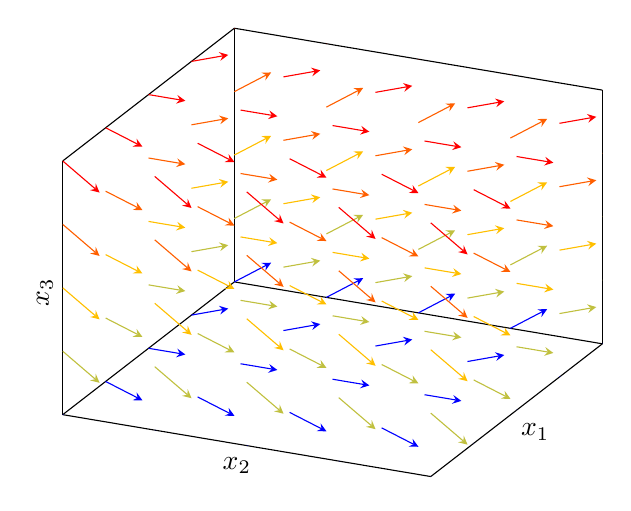
\begin{tikzpicture}
  \begin{axis}[
    domain=-1:1,
    samples=10,
    xmin=-1,xmax=1,
    ymin=-1,ymax=1,
    zmin=-1,zmax=1,
    ticks=none,
    zlabel=$x_3$,
    ylabel=$x_1$,
    xlabel=$x_2$
    ]
    \pgfplotsinvokeforeach{-1,-.5,0,.5,1}{
      \addplot3[quiver,-stealth,
        samples=5,
      %point meta={sqrt((x)^2+(y)^2+(z)^2)},
      quiver={
        u={1},
        v={0},
        w={y},
        colored, scale arrows=.2}]
      (x,y,#1);
    }
  \end{axis}
\end{tikzpicture}\end{center}

\item Rozważmy teraz $M=\R^3$ oraz pole wektorowe 
  $$X(x, y)=x\frac{\partial}{\partial y}-y\frac{\partial}{\partial x}$$
  jak w przykładzie z poprzedniego rozdziału. Wówczas 
  $$\phi_t^X(x, y)=(x\cos t-y\sin t, x\sin t+y\cos t)$$

\begin{illustration}
\begin{axis}[
    xmin = -3, xmax = 3,
    ymin = -3, ymax = 3,
    zmin = 0, zmax = 1,
    axis equal image,
    axis lines = middle,
    xtick distance = 1,
    ytick distance = 1,
    ticks = none,
    view = {0}{90},
    scale = 1.25,
    %title = {\bf Vector Field $F = [-y,x]$},
    height=7cm,
    %xlabel = {$x$},
    %ylabel = {$y$},
    colormap/viridis,
    %colorbar,
    %colorbar style = {
    %    ylabel = {Vector Length}
    %}
]
 
\addplot3[
    point meta = {sqrt(x^2+y^2)},
    quiver = {
        %u = {-y/sqrt(x^2+y^2)},
        %v = {x/sqrt(x^2+y^2)},
        u = {-y},
        v = {x},
        scale arrows = 0.4,
    },
    quiver/colored = {mapped color},
    -stealth,
    domain = -2:2,
    domain y = -2:2,
    samples=7,
    thick
] {0};
 
\end{axis}
\end{illustration}
  
$$d(\phi_t^X)_p:T_p\R^2\to T_{\phi_t^X(p)}\R^2$$
jest zadana macierzą obrotu o $t$ stopni
$$d(\phi_t^X)=\begin{bmatrix}\cos t&-\sin t\\\sin t &\cos t\end{bmatrix}$$
W takim razie macierz odwzorowania odwrotnego to
$$(d(\phi_t^X)_p)^{-1}=\begin{bmatrix}\cos t & \sin t\\-\sin t & \cos t\end{bmatrix}$$

Rozważmy teraz pole wektorowe $Y(x,y)=\frac{\partial}{\partial x}=(1, 0)$. Wtedy pochodna Liego $Y$ to
\begin{align*}
  \frac{d}{dt}_{t=0}Y(\phi_t^X(x,y))=&\frac{d}{dt}_{t=0}\begin{bmatrix}\cos t & \sin t\\-\sin t & \cos t\end{bmatrix}\begin{bmatrix}1\\0\end{bmatrix}=\\
  =&\frac{d}{dt}_{t=0}\begin{bmatrix}\cos t\\-\sin t\end{bmatrix}=\begin{bmatrix}\sin 0\\-\cos 0\end{bmatrix}=\begin{bmatrix}0\\-1\end{bmatrix}=-\frac{\partial}{\partial y}=L_X(Y)(x,y)
\end{align*}

Warto zauważyć, że $X(0,0)=0$, a jednak $L_XY(0,0)\neq 0$.
\end{example}

\subsection{Własności}

\begin{theorem}
  $$L_XY=[X,Y]$$
\end{theorem}

\begin{proof}
  Pokażemy, że dla każdego $p\in M$ $L_XY(p)=[X,Y](p)$. Rozbijemy to na przypadki w zależności od tego, czy $X(p)$ jest zerowe czy nie.

  \begin{enumerate}
    \item $\mathbf{\color{blue}X(p)\neq0}$ 

      Z \hyperref[wyprostowanie pola wektorowego]{przykładu o wyprostowywaniu pola wektorowego}\marginpar{Dla każdego pola wektorowego $X$ możemy znaleźć mapę taką, że $X=\frac{\partial}{\partial x_1}$ po wyrażeniu w tej mapie.} wiemy, że możemy dobrać mapę, w której 
      $$X(x_1,...,x_n)=\frac{\partial}{\partial x_1}$$
      oraz $p=(0,...,0)$. Niech $Y(x)=\sum_{i\leq n}Y_i(x)\frac{\partial}{\partial x_i}$ w tej mapie. Komutator $X$ i $Y$ w takim przypadku wynosi $[X,Y]=\sum\frac{\partial Y_j}{\partial x_1}(0)\cdot\frac{\partial}{\partial x_j}$, bo $X$ ma wszystkie pochodne zerowe i niezerową wartość tylko na pierwszej współrzędnej:
      \begin{align*}
        [X,Y](0)=\sum\left[\sum\left[X_i(0)\frac{\partial Y_j}{\partial x_i}(0)-Y_i(0)\frac{\partial X_j}{\partial x_i}(0)\right]\right]=\sum_{j\leq n}\frac{\partial Y_j}{\partial x_1}(0)\cdot \frac{\partial}{\partial x_j}
      \end{align*}
      
      Do wyliczenia pochodnej Liego potrzebujemy potoku pola $X$
      $$\phi_t^X(x_1,...,x_n)=(x_1+t,x_2,...,x_n)$$
      oraz jego pochodnej, czyli $d\phi_t^X=id_{\R^n}=(d\phi_t^X)^{-1}$. Podstawiając do definicji otrzymujemy
      \begin{align*}
        L_XY(0)=&\frac{d}{dt}_{t=0}(d\phi_t^X)^{-1}Y(\phi_t^X(0))=\\
        =&\frac{d}{dt}_{t=0}(d\phi_t^X)^{-1}Y(t,0,...,0)=\\
        =&\frac{d}{dt}Y(t,0,...,0)=\frac{\partial}{\partial x_1}Y(0)=[X,Y](0)
      \end{align*}
  \end{enumerate}

  Czyli po takim wyrażeniu $X$ i $Y$ w mapie mamy $[X,Y](p)=L_XY(p)$.

\item $\mathbf{\color{blue}X(p)=0}$

  Zaczniemy od udowodnienia dwóch faktów pomocniczych.

  \textbf{Fakt 1.} Jeśli $X:(a,b)\to T_pM$ oraz $f:M\to \R$ są gładkimi funkcjami, to $\frac{d}{dt}[X(t)f]=[\frac{d}{dt}X(t)]f$.

  \begin{align*}
    \frac{d}{dt}[X(t)f]=&\lim_{\varepsilon\to 0}\frac{X(t+\varepsilon)f-X(t)f}{\varepsilon}=\\
    =&\lim_{\varepsilon\to 0}\left[\frac{X(t+\varepsilon)-X(t)}{\varepsilon}\cdot f\right]\overset{\star}{=}\\
     &=\left[\lim_{\varepsilon\to0}\frac{X(t+\varepsilon)-X(t)}{\varepsilon}\right]\cdot f=\left[\frac{d}{dt}X(t)\right]f
  \end{align*}
  Równość $\star$ wynika z ciągłości pochodnej kierunkowej względem kierunku.

  \textbf{Fakt 2.} Dla $X\in C^\infty(TM)$, $f\in C^\infty(M)$ oraz dyfeomorfizmu $h:M\to N$ rozważmy pole wektorowe $dh(X)\in C^\infty(TN)$ oraz funkcję $f\circ h^{-1}\in C^\infty(N)$ przeniesione na $N$ przez $h$. Wówczas
    $$Xf(p)=dh(X)(fh^{-1})(h(p)).$$

%    \marginpar{Dowód Faktu 2. jest ćwiczeniem, tutaj }
%    Dowód pozostawiamy jako ćwiczenie.
    
%    Zgodnie z definicją podaną w 5.2 dla dowolnego $p\in M$ mamy
%    \begin{align*}
%      dh(X_{(fh^{-1})(h(p))}=&dh_{h^{-1}(fh^{-1}(h(p))}(X_{h^{-1}fh^{-1}(h(p)})=\\
%      =&dh_{h^{-1}(f(p))}(X_{h^{-1}(f(p))})
%    \end{align*}

%    Niech $X_{f(p)}=[c, t]$, wówczas $dh(X)(fh^{-1}(h(p))=dh(X)(f(h^{-1}h(p))=dh(X)f(p)=[$
%    \begin{align*}
%      [dh(X)](fh^{-1})(h(p))=&[dh(X)](h^{-1})(h(p))+h^{-1}[dh(X)]f(h(p))=\\
%      =&fdh(X)(p)+
%    \end{align*}

    Da $q\in N$ mamy\marginpar{Jak w \hyperref[przeniesione pole wektorowe]{podrozdziale 5.2 o przenoszeniu pól wektorowych przez dyfeomorfizmy.}}
    $$dh(X)=dh_{h^{-1}(q)}(X(h^{-1}(q)))$$
    ale ponieważ $h$ jest dyfeomorfizmem, to zawsze istnieje $p\in M$ takie, że $q=h(p)$. Możemy więc zapisać
    $$dh(X)=dh_{h^{-1}(h(p))}(X(h^{-1}(h(p))))=dh_p(X(p)).$$
    W takim razie
    \begin{align*}
      dh(X)(fh^{-1})(h(p))=&d_p(X(p))(fh^{-1})(h(p))=d_pX(fh^{-1}(h(p)))=d_pX(f(p))=Xf(p)
    \end{align*}
    tak jak chcieliśmy.

    Niech $f$ będzie dowolną funkcją gładką na rozmaitości $M$. Zadziałamy na nią wektorami $[X,Y](p)$ oraz $L_XY(p)$
    \begin{align*}
      [X,Y](p)f=&[X,Y]f(p)=XYf(p)-YXf(p)=-YXf(p)
    \end{align*}
    bo $X(p)=0$. Ponieważ $X(p)=0$, to na pewnym otoczeniu $p$ mamy $\phi_t^X(p)=p$ dla każdego $p$. Czyli
    \begin{align*}
      (L_XY)f(p)=&(L_XY)_pf=\left[\frac{d}{dt}_{t=0}d\phi_{-t}^X[Y(\phi_t^X(p))]\right]f=\\
      =&\left[\frac{d}{dt}_{t=0}d\phi_{-t}^X[Y(p)]\right]f\overset{F.1}{=}\frac{d}{dt}_{t=0}[d\phi_{-t}^X(Y)f(p)]\overset{F.2}{=}\\
      =&\frac{d}{dt}_{t=0}\left[Y(f\phi_{-t}^X)(\phi_t^X(p))\right]=\frac{d}{dt}[Y(f\phi_{-t}^X)(p)]=\\
      =&\frac{d}{dt}_{t=0}\frac{d}{ds}_{s=0}[f\phi_{-t}^X(\phi_s^Y(p))]=\frac{d}{ds}_{s=0}\frac{d}{dt}_{t=0}[f\phi_{-t}^X\phi_s^Y(p)]=\\
      =&\frac{d}{ds}_{s=0}-Xf(\phi_s^Y(p))=Y(-Xf(p))=-yXf(p)=[X,Y]f(p)
    \end{align*}
  
\end{proof}

Pochodna Liego ma \acc[b]{następujące własności}, które wynikają z własności komutatora:\marginpar{Własności komutatora zostały przedstawione pod \hyperref[komutator-definicja]{Definicją 6.2}}
\begin{multicols}{2}
\begin{enumerate}
  \item $L_XY=-L_YX$
  \item $L_X[Y,Z]=[L_xY,Z]+[Y,L_XZ]$ %(reguła Leibniza dla komutatora i pochodnej Liego)
  \item $L_X(Y+Z)=L_XY+L_XZ$%\columnbreak
  \item $L_{X+Y}Z=L_XY+L_YZ$
  \item $L_X(fY)=XfY+fL_XY$
  \item $L_{fX}Y=fL_XY-(Yf)X$
\end{enumerate}
\end{multicols}

\subsection{Komutowanie potoków}

\begin{definition}
  Lokalne potoki pól $X,Y$ na $M$ \important{komutują} na otoczeniu  punktu $p\in M$, jeśli istnieje $\varepsilon>0$ taki, że dla każdego $|t|,|s|<\varepsilon$ zachodzi
  \marginpar{Lee podaje $[X,Y]=0$ jako definicję komutowania potoków pól $X$ i $Y$. My podchodzimy do problemu najpierw we współrzędnych lokalnych, a dopiero potem przechodzimy do perspektywy całego $M$.}
  $$\phi_s^Y\circ\phi_t^X(q)=\phi_t^X\circ\phi_s^Y(q)$$
  dla $q$ bliskich punktowi $p$.
\end{definition}

%Oznacza to, że $YXf=XYf$ dla wszystkich $f$ gładkich na otoczeniu $p$.

\begin{theorem}
  Lokalne potoki pól $X,Y$ komutują na otoczeniu punktu $p$ $\iff$ $[X,Y]\equiv 0$ na pewnym otoczeniu punktu $p$. Oznacza to również, że $L_XY=0$ na otoczeniu punktu $p$.
\end{theorem}

\begin{proof}
  $\impliedby$

  Potrzebujemy faktu pomocniczego:

  Jeśli $\phi:M_1\to M_2$ jest dyfeomorfizmem i $X_1$ jest polem na $M_1$, a $X_2=d\phi(X_1)$ jest polem na $M_2$, to wówczas $\phi$ przenosi trajektorie pola $X_1$ na trajektorie pola $X_2$. Oznacza to, że
  $$\phi(\phi_t^{X_1}(p))=\phi_t^{X_2}(\phi(p))$$

  Zakładamy, że $L_XY=[X,Y]=0$. Możemy pokazać, że dla każdego $q\in M$ w pobliżu $p$ oraz $t_0$ bliskich $0$ mamy
  %$$0=\lim_{t\to 0}\frac{d\phi_{-t}^X[Y(\phi_t^X(p))]-Y(p)}{t}$$
  %$$0=\frac{d}{dt}_{t=0}d\phi_{-t}^X[Y(\phi_t^X(p))]$$
%
%  $$0=[X,Y]f=XYf-YXf\implies XYf=YXf$$
%  Wiemy, że $d\phi_t^X(p)=X(\phi_t^X(p))$ dla każdego $p$ oraz $t$ jako, że są to krzywe całkowe pola $X$. Czyli jeśli $X(Yf)=Y(Xf)$ dla każdego $f$, to musi być 
%  $$d\phi_t^X(Y)=Y.$$
%  W takim razie $\phi_t^X$ nałożone na trajektorie $Y$ daje nadal trajektorie $Y$, stąd potoki pola $X$ i $Y$ są względem siebie przemienne (tzn. $\phi_t^X\phi_s^Y=\phi_s^Y\phi_t^X$) i pola te komutują.
  $$\frac{d}{dt}_{t=t_0}(d\phi_{-t}^X)(Y(\phi_t^X(q))=\phi_{t_0}^X(q)$$
  To z kolei jest równe zero, bo
  \begin{align*}
    \frac{d}{dt}_{t=t_0}(d\phi_{-t}^X)(Y(\phi_t^X(q)))=&-\frac{d}{ds}_{s=0}(d\phi_{-t_0-s}^X)Y(\phi_{t_0+s}^X(q))=\\
    =&\frac{d}{ds}_{s=0}(d\phi_{-t_0}^X)(d\phi_{-s}^X)Y(\phi_s^X(\phi_{t_0}^X(q)))=\\
    =&(d\phi_{-t_0^X}\frac{d}{ds}_{s=0}(d\phi_{-s}^XY(\phi_s^X(\phi_{t_0}^X(q))=\\
    =&(d\phi_{-t_0}^X)[L_XY(\phi_{t_0}^X(q))]=\\
    =&(d\phi_{-t_0}^X)(0)=0
  \end{align*}

  Jeśli scałkujemy $L_XY$ od $0$ do $t$, dla małego $t$, to tak naprawdę całkujemy funkcję stale równą zero i dostajemy
  \begin{align*}
    0=&\int_0^{t} \frac{d}{ds}_{t=0}(d\phi_{-s}^X)(Y(\phi_s^X(q)))ds=\\
    =&(d\phi_{-t}^X)(Y(\phi_t^X(q))-(d\phi_0^X)(Y(\phi_0^X(q)))=\\
    =&(d\phi_{-t}^X)(Y(\phi_t^X(q)))-Y(q)
  \end{align*}
  bo $\phi_0^X=id$. Dla $q$ bliskich $p$ oraz małych $t$ dostajemy więc
  $$Y(q)=(d\phi_{-t}^X)(Y(\phi_t^X(q)))$$

  Zatem lokalny dyfeomorfizm $\phi_t^X$ przenosi pole $Y$ na siebie, a więc trajektorie pola $Y$ są przez niego przenoszone na trajektorie $Y$. Mamy więc
  $$\phi_t^X(\phi_s^Y(q))=\phi_s^Y(\phi_t^X(q))$$
  dla $q$ bliskich $p$ oraz małych $s$. W takim razie potoki $X$ i $Y$ komutują na otoczeniu punktu $p$.

  $\implies$

  Zauważmy najpierw, że jeśli dyfeomorfizm $\phi$ zachowuje trajektorie pola $Y$, tzn. $\phi(\phi_t^Y(q))=\phi_t^Y(\phi(q))$ dla wszystkich $q$, to pole $Y$ jest $\phi$-niezmiennicze. To znaczy $d\phi(Y)=Y$. Dokładniej mamy dla każdego $q$ $d\phi(Y(q))=Y(\phi(q))$ lub $Y(q)=(d\phi)^{-1}(Y(\phi(q)))$.

  Zakładamy, że $\phi_t^X\phi_s^Y=\phi_s^Y\phi_t^X$, czyli $\phi_t^X$ i $\phi_s^Y$ komutują wokół $p$. Wówczas dla małych $t$ $\phi_t^X$ przenosi małe kawałki trajektorii pola $Y$ w pobliżu $p$ na małe kawałki trajektorii pola $Y$. Dzięki faktowi wyżej wiemy, że wówczas
  $$(d\phi_t^X)Y(q)=Y(\phi_t^X(q)),$$
  czyli
  $$Y(q)=Y(\phi_{-t}^X(\phi_t^X(q)))=(d\phi_{-t}^X)(Y(\phi_t^X(q)))$$
  Dalsze rachunki dają
  $$L_XY(q)=\frac{d}{dt}_{t=0}(d\phi_{-t}^X)Y(\phi_t^X(q))=\frac{d}{dt}_{t=0}Y(q)=0$$
  czyli to co chcieliśmy.
\end{proof}

\subsection{Wyprostowanie komutujących pól wektorowych}

\begin{theorem} 
  Niech $X_1,...,X_k$ będą polami wektorowymi na $M$, a $dim(M)=m\geq k$. Załóżmy, że dla $q$ w otoczeniu punktu $p\in M$ pola $X_i$ 
  \begin{itemize}
    \item parami komutują oraz 
    \item są liniowo niezależne, tzn. dla $q\in M$ blisko $p$ układ $X_1(q),...,X_k(q)$ wektorów jest liniowo niezależny w $T_qM$.
  \end{itemize}

  Wówczas istnieje mapa $\phi$ wokół $p$, w której pola $X_i$ mają postać
  $$X_i(x_1,...,x_m)=\frac{\partial}{\partial x_i}$$
\end{theorem}

\begin{proof}
  Ponieważ działamy lokalnie wokół $p$, możemy przyjąć, że $M=\R^m$, $p=(0,...,0)$ oraz
  $$X_i(x)=\sum (X_i)_j(x)\cdot\frac{\partial}{\partial x_j}.$$
  Ponieważ $X_1(p),...,X_k(p)$ są liniowo niezależne, to macierz
  $$\begin{bmatrix}(X_1)_1 & (X_2)_1 & ... &\hdots (X_k)_1\\(X_1)_2 & (X_2)_2 & \hdots (X_k)_2\\
  \vdots & \vdots & \ddots & \hdots\\(X_1)_m & (X_2)_m) & \hdots & (X_k)_m\end{bmatrix}$$
  ma rząd $k$. Przyjmijmy więc, że wiersze od $1$ do $k$ tworzą macierz nieosobliwą. Możemy to zrobić, bo przenumerowanie współrzędnych nic nie psuje. Rozważmy odwzorowanie
$$\lambda(t_1,...,t_m)=\phi_{t_1}^{X_1}\circ\phi_{t_2}^{X_2}\circ...\circ\phi_{t_k}^{X_k}(0,...,0,t_{k+1},...,t_m).$$
$\lambda$ jest gładko określone na pewnym otoczeniu $(0,...,0)$ oraz
$$\lambda(0,...,0)=(0,...,0)=p.$$

Gdy $k=2$, a $m=3$, to $\lambda(x,y,z)=\phi_x^{X_1}\phi_y^{X_2}(0,0,z)$, z drugiej strony mamy równość
$$\phi_x^{X_1}\phi_y^{X_2}(0,0,z)=\phi_y^{X_2}\phi_x^{X_1}(0,0,z)$$
która wynika z rysunku

\begin{illustration}
  \draw[->] (0,0)--(0, 2);
  \draw[->] (0,0)--(3,0);
  \draw[->] (0,0)--(-0.75, -1);

  \filldraw[color=white, pattern color=green!60, pattern=crosshatch] (-0.5, 1.2)--(2.5, 1.95)--(3.25, 0)--(0.25, -0.75)--cycle;
    
\filldraw (0, 1) circle (1.5pt);
\filldraw (2, 1.5) circle (1.5pt);
\filldraw (2.5,0.2) circle (1.5pt);
\filldraw (0.5, -0.3) circle (1.5pt);

  \draw plot coordinates {(0, 1) (2, 1.5) (2.5, 0.2) (0.5, -0.3) (0, 1)};
  \draw[->](0, 1)--(1, 1.25);
  \draw[->](2, 1.5)--(2.25, 0.85);
  \draw[->] (2.5, 0.2)--(1.5, -0.05);
  \draw[->] (0.5, -0.3)--(0.25, 0.35);

  \node at (-0.5, 1) {$(0,0,z)$};
  \node at (2.3, 1.8) {$\phi_y^{X_2}(0,0,z)$};
  \node at (3.5, -0.2) {$\phi_y^{X_2}\phi_x^{X_1}(0,0,z)=\phi_x^{X_1}\phi_y^{X_2}(0,0,z)$};
  \node at (0.5, -0.6) {$\phi_x^{X_1}(0,0,z)$};
\end{illustration}

Obliczmy pochodną $\frac{\partial \lambda(t_1,...,t_m)}{\partial t_i}$ dla $i=1,...,k$
\begin{align*}
  \frac{\partial \lambda(t_1,...,t_m)}{\partial t_i}=&\frac{d}{ds}_{s=0}\phi_{t_1}^{X_1}\circ...\circ\phi_{t_i+s}^{X_i}\circ...\circ\phi_{t_k}^{X_k}(0,...,0,t_{k+1},...,t_m)=\\
  =&\frac{d}{ds}_{s=0}\phi_{t_i+s}^{X_i}\circ\phi_{t_i}^{X_1}\circ...\circ\phi_{t_k}^{X_k}(0,...,0,t_{k+1},...,t_m)=\\
  =&\frac{d}{ds}_{s=0}\phi_s^{X_i}(\phi_{t_1}^{X_1}\circ...\circ\phi_{t_i}^{X_i}\circ...\circ\phi_{t_k}^{X_k}(0,...,0,t_{k+1},...,t_m))=\\
  =&\frac{d}{ds}_{s=0}\phi_s^{X_i}(\lambda(t_1,...,t_m))=\\
  =&X_i(\lambda(t_1,...,t_m))
\end{align*}
Ponieważ $\lambda(0,...,0,t_{k+1},...,t_m)=(0,...,0,t_{k+1},...,t_m)$, to $D\lambda(0)$ zapisuje się jako macierz
$$D\lambda(0)=
\left[
  \begin{array}{c | c}
    \begin{array}{c c c}
      (X_1)_1 &\hdots & (X_k)_1\\
      \vdots & \ddots & \vdots \\ %& & & \makebox(0,0){\text{\huge0}}\\
      (X_1)_k & \hdots & (X_k)_k\\
          %& & & 1\\
      \vdots & \ddots & \vdots \\ % & 0 & 1 \\
         %& & & 0 & 0& 1\\
        (X_1)_m & \hdots & (X_k)_m %& 0 & 0 & \hdots & 1
  \end{array} & 
    \begin{array}{c}
        \makebox(0,0){\text{\huge0}}\\
          \\
          \\
      \hline
      \\
      \begin{array}{c c c c}
        1\\
        0 & 1\\
        0 & 0 & \hdots & 1
      \end{array}
    \end{array}
  \end{array}
\right]
$$
Łatwo zobaczyć, że $D\lambda(0)$ jest macierzą nieosobliwą, więc $\lambda$ jest dyfeomorfizmem na otoczeniu $0$. Ponieważ 
$$d\lambda(\frac{\partial}{\partial t_i}(t_1,...,t_m))=X_i(\lambda(t_1,...,t_m),$$
to dla mapy $\phi=\lambda^{-1}$ mamy
$$d\phi(X_i(\lambda(t_1,...,t_m))=\frac{\partial}{\partial t_i}(t_1,...,t_m)$$
czyli $X_i=\frac{\partial}{\partial t_i}$ w tej mapie.
\end{proof}

\newpage

\section{Rozmaitości orientowalne}

\subsection{Orientacja w przestrzeni wektorowej $V$ wymiaru $n$}

Niech $B(V)$ będzie zbiorem wszystkich baz $b=(v_1,...,v_n)$ przestrzeni $V$. Dla baz $b_1=(v_1,...,v_n)$ oraz $b_2=(w_1,...,w_n)$ macierz przejścia $M_{b_1,b_2}=(a_{ij})_{n\times m}$ to taka macierz, że $w_k=\sum a_{ik}v_i$. Równoważnie jest to macierz przekształcenia $V\to V$ takiego, że $v_i\mapsto w_i$, czyli wyrażenia wektorów zapisanych za pomocą $w_i$ w bazie $b_1$. Macierz $M_{b_1,b_2}$ jest macierzą nieosobliwą. Opiszmy więc relację na $B(V)$
$$b_1\sim b_2\iff \det(M_{b_1,b_2})>0$$

\begin{lemma}
  Relacja $b_1\sim b_2\iff \det(M_{b_1,b_2})>0$ jest relacją równoważności która ma dwie klasy abstrakcji.
\end{lemma}

\begin{proof}$ $

  Zaczniemy od udowodnienia, że jest to relacja równoważności:
  \begin{description}
    \item[zwrotność:] $M_{b,b}=I_{n\times n}$, a z kolei $\det(I)=1>0$
    \item[symetryczność:] zauważmy, że $M_{b_2,b_1}=M_{b_1,b_2}^{-1}$, czyli $\det(M_{b_2,b_1})=\frac{1}{\det(M_{b_1,b_2})}$.
    \item[przechodniość:] wynika z prostej kalkulacji $M_{b_1,b_3}=M_{b_1,b_2}\cdot M_{b_2,b_3}$ oraz
      $$\det(M_{b_1,b_3})=\det(M_{b_1,b_2})\det(M_{b_2,b_3})$$
  \end{description}

  Relacja ta ma dwie klasy abstrakcji, bo jeśli $b_1\not\sim b$ oraz $b_2\not\sim b$, to wówczas tak jak przy przechodniości $M_{b_1,b_2}=M_{b_1,b}\cdot M_{b,b_2}$ i $\det(M_{b_1,b_2})$ jako iloczyn dwóch wartości ujemnych jest dodatni. Stąd $b_1\sim b_2$.
\end{proof}

\begin{definition}
  \important{Orientacją} na przestrzeni wektorowej $V$ nazywamy dowolną klasę abstrakcji relacji $\sim$ jak wyżej na zbiorze $B(V)$.
\end{definition}

Następujące operacje na bazie $b=(v_1,...,v_n)$ dają bazy z tej samej klasy abstrakcji (tj. macierz przejścia ma dodatni wyznacznik)
\begin{itemize}
  \item parzysta permutacja wektorów bazy (złożenie parzystej liczby transpozycji)
  \item mnożenie wektorów z bazy przez dodatnie współczynniki
  \item zamiana jednego z wektorów $v_k$ na wektor
  $$v_k'=v_k+\sum_{i\neq k}a_iv_i$$
  dla parzystych współczynników $a_i\in \R$
  \item dowolne kombinacje operacji wymienionych wyżej
  \item dowolna ciągła modyfikacja bazy (w przestrzeni baz)
\end{itemize}

W przestrzeni $\R^3$ klasy abstrakcji rozpoznaje się za pomocą reguły śruby prawoskrętnej. W $\R^2$ natomiast klasy orientacji są zadane przez kierunek obrotu (o kąt $<\pi$) drugiego wektora bazy względem pierwszego wektora bazy, zgodny lub przeciwny do ruchu wskazówek zegara.

Następujące modyfikacje bazy $b=(v_1,...,v_n)$ wyprowadzają ją poza klasę abstrakcji, czyli zmieniają orientację:
\begin{itemize}
  \item nieparzysta permutacja wektorów bazy, np. transpozycja dowolnych dwóch wektorów
  \item pomnożenie jednego z wektorów bazy przez ujemny współczynnik
\end{itemize}
\bigskip

Na rozmaitości $M$ każda mapa $(U,\phi)$ zadaje dla każdego $p\in U$ orientację w przestrzeni stycznej $T_pM$ przez klasę abstrakcji bazy $(\frac{\partial}{\partial\phi_1}(p),...,\frac{\partial}{\partial\phi_n}(p))$. Dwie mapy $(U,\phi)$ oraz $(V,\psi)$ \important{zadają tę samą orientację na przestrzeni $T_pM$} dla $p\in U\cap V$ wtedy, gdy Jakobian odwzorowania przejścia
$$\left[\frac{\partial(\phi\psi^{-1})_k}{\partial x_j}(\psi(p))\right]_{j,k}$$
ma dodatni wyznacznik. Jest to macierz przejścia z bazy $\left(\frac{\partial}{\partial\psi_i}\right)$ do bazy $\left(\frac{\partial}{\partial\phi_i}\right)$.

\begin{definition}$ $
  \begin{enumerate}
    \item \important{Orientacją} rozmaitości $M$ nazywamy wybór atlasu $\set{A}=\{(U_\alpha,\phi_\alpha)\}$ dla $M$, takiego że każde dwie mapy $(U_\alpha,\phi_\alpha),(V_\beta,\psi_\beta)$ mają dodatni wyznacznik jakobianu odwzorowania przejścia $\phi\psi^{-1}$ w każdym punkcie $p\in U_\alpha\cap V_\beta$.
    \item Rozmaitość jest \important{orientowalna}, jeśli posiada atlas jak wyżej. W przeciwnym razie jest \acc[b]{nieorientowalna}.
    \item Dwa atlasy $\set{A}_1,\set{A}_2$ jak wyżej zadają tę \acc[i]{samą orientację}, jeśli dla każdej mapy $(U,\phi)\in \set{A}_1$ i dla każdej mapy $(V,\psi)\in\set{A}_2$ jakobian odwzorowania przejścia $\phi\psi^{-1}$ ma dodatni wyznacznik w każdym punkcie $p\in U\cap V$.
  \end{enumerate}
\end{definition}

\begin{remark}
  Jeśli rozmaitość $M$ jest orientowalna i spójna, to można na niej zdać dokładnie $2$ różne orientacje. 

  Co więcej, można powiedzieć, że jeśli $M$ jest orientowalna, to $M$ jest spójna $\iff$ $M$ posiada 2 orientacje.
\end{remark}

\begin{proof}{\color{red}\large To wymaga dowodu}
%
%  \textbf{Orientowalność, posiada co najmniej 2}
%
%  Chyba mogę wejść sobie najpierw w $\R^{n}$, tam coś porobić na $T_pM$ wyrażonym w lokalnych współrzędnych i potem chuju muju kurwa ciulu?
%
%  \textbf{Co najwyżej 2 struktury}
%
%  Załóżmy, że mamy $\set{A}_1,\set{A}_2,\set{A}$ atlasy jak w punkcie 1. wyżej na rozmaitości $M$ takie, że istnieją mapy $(U,\phi)\in \set{A}_1,(V,\psi)\in\set{A}_2$ oraz $(W,\theta)\in\set{A}$ takie, że $\phi\theta^{-1}$ i $\theta\psi^{-1}$ mają ujemny wyznacznik jakobianu. Fakt z analizy mówi, że jakobian 
%  $$\phi\psi^{-1}=(\phi\theta^{-1})(\theta\psi^{-1})$$ 
%  jest iloczynem jakobianów poszczególnych funkcji, stąd
%  $$\det(D\phi\psi^{-1})=\det(D\phi\theta^{-1}\circ D\theta\psi^{-1})=\det(D\phi\theta^{-1})\cdot\det(D\theta\psi^{-1})>0$$
%  jako iloczyn dwóch wartości ujemnych. Stąd jeśli $\set{A}_1\not\sim\set{A}$ i $\set{A}_2\not\sim\set{A}$ oznacza, że musi być $\set{A}_1\sim\set{A}_2$, gdzie $\sim$ rozumiemy jako posiadanie przez atlasy tej samej orientacji.

  Udowodnimy tylko pierwszą wersję uwagi.

  Niech $M$ będzie orientowalną i spójną rozmaitością. Wówczas na $M$ istnieje atlas $\set{A}$ taki, że każde dwie mapy na nim mają odwzorowanie przejścia z dodatnim wyznacznikiem jakobianem w każdym punkcie. Skupmy się na jednej takiej mapie, $(U,\phi)\in\set{A}$. Zadaje ona bazę $\left(\frac{\partial}{\partial\phi_1},...,\frac{\partial}{\partial\phi_n}\right)$ na $T_pM$ dla $p\in U$. Możemy ją przenieść na $\R^n$ poprzez $\phi^*_p$, niech $(v_1,...,v_n)$ będą odpowiadającymiiiiiii
\end{proof}

\begin{fact}
  Rozmaitość $M$ jest \acc[b]{nieorientowalna} $\iff$ istnieje ciągła droga $b(t):[0,1]\to B(M)$ taka, że $b(0),b(1)\in T_pM$ oraz $b(0)\not\sim b(1)$ w $T_pM$.
\end{fact}

\newpage

\section{Podrozmaitości}

\begin{definition}
  Podzbiór $N\subseteq M^n$ dla gładkiej rozmaitości $M$ jest \important{podrozmaitością wymiaru $n$}, jeśli każdy punkt $p\in N$ posiada mapowe otoczenie otwarte $U_p\subseteq M$ oraz mapę $\phi:U_p\to V=\phi(U_p)\subseteq\R^m$ takie, że
  $$\phi(U_p\cap N)=\{(x_1,...,x_m)\in V\;:\;x_{n+1}=...=x_m=0\}$$
\end{definition}

\begin{illustration}
  %\draw[orange, step=0.2] (-2, -2) grid (6, 6);

  \path (-1, -2) edge [bend left=20] (1, -1.5);
  \path (1, -1.5) edge [bend right=20] (0.5, 0.5);
  \path (0.5, 0.5) edge [bend right=20] (-1.5, 0);
  \path (-1.5, 0) edge [bend left=20] (-1, -2);

  %\filldraw[pattern=crosshatch] (0, -0.3) circle (0.5);
  \filldraw[color=orange, pattern=crosshatch, pattern color=orange, smooth cycle, rounded corners=0.5mm] plot coordinates{(-0.5, -0.3) (-0.1, -0.8) (0.7, -0.2) (0, 0.3)};

  \draw[->] (3, -0.5)--(3, 3.5);
  \draw[->] (1, 1.5)--(5, 1.5);

  \draw[orange, pattern={Stars[points=7, angle=20, radius=3pt, distance=7pt]}, pattern color = orange!40] (3, 1.5) circle (1.3);

  \path (-1, 1) edge [bend left=10] (-0.2, 0.3);
  \node at (-1.2, 1.3) {$\color{orange}U_p$};

  \node at (-1.3, -2) {$M$};
  \path[very thick, green] (-1, -1.2) edge [bend right=30] (-0.2, -0.5);
  \path[very thick, green] (-0.2, -0.5) edge [bend left=30] (0.6, 0.4);
  \node at (-0.8, -0.8) {$\color{green}N$};

  \draw[ultra thick, green] (1.7, 1.5)--(4.3, 1.5);
  \draw[ultra thick, green] (1.7, 1.55)--(4.3, 1.55);
  \draw[ultra thick, green] (1.7, 1.45)--(4.3, 1.45);

  \node (A) at (4, -0.5) {$\color{green}\phi(U_p\cap N)$};
  \path [<-, green] (3.5, 1.4) edge [bend right=10] (A);

  \path[->] (0.2, -0.3) edge [bend right=20] node [midway, above] {$\phi$} (2, 1);

  \node at (3.4, 3.3) {$\R^{m-n}$};
  \node at (4.7, 1.2) {$\R^n$};
  \node at (2, 0) {$\R^m$};

  \node at (4.3, 2.3) {$\color{orange}V$};
\end{illustration}

Możemy to również rozumieć, że wokół każdego $p\in N$ istnieje lokalny układ współrzędnych $(x_1,...,x_m)$ na otwartym otoczeniu $U_p\subseteq M$ taki, że $U_p\cap N$ wyraża się w tym układzie jako $\{x_{n+1}=...=x_m=0\}$.

\begin{remark}
  Każda $n$-wymiarowa podrozmaitość $N\subseteq M^m$ jest $n$-wymiarową gładką rozmaitością.
\end{remark}

\begin{proof}
  Wybierzemy na $N$ atlas, a następnie udowodnimy jego zgodność.

  Jako mapy wybierzemy pary postaci $(U_p\cap N, \Pi_n^m\circ \phi)$, gdzie $(U_p,\phi)$ są mapami na $M$ jak w definicji wyżej, natomiast 
  $$\Pi_n^m:\R^m\to \R^n$$
  jest rzutowaniem, tzn:
  $$\Pi_n^m(x_1,...,x_n,x_{n+1},...,x_m)=(x_1,...,x_n).$$
  W takim razie $\Pi_n^m\circ\phi$ to pierwsze $n$ współrzędnych gładkiej mapy $\phi$, czyli jest gładką funkcją z $N$ w $\R^n$.

  \begin{illustration}
    %\draw[orange, step=0.2] (-2, -2) grid (6, 6);

    \path (-1, -2) edge [bend left=20] (2, -1.5);
    \path (2, -1.5) edge [bend right=20] (1.5, 0.5);
    \path (1.5, 0.5) edge [bend right=20] (-1.5, 0);
    \path (-1.5, 0) edge [bend left=20] (-1, -2);

    \path[very thick, green] (-1, -1.2) edge [bend right=30] (0.3, -0.5);
    \path[very thick, green] (0.3, -0.5) edge [bend left=30] (1.6, 0.4);
    
    \draw (-0.1, -0.5) ellipse (0.6 and 0.5);
    \node at (-0.7, -1) {$U_p$};
    \filldraw (0.1, -0.75) circle (1.5pt) node [below] {$p$};

    \path[->] (0.1, -0.6) edge [bend left=60] node [midway, above] {$\psi=\Pi_n^m\phi$} (2.2, 0.9);

    \draw[rotate around={30:(0.7, -0.2)}] (0.7, -0.2) ellipse (0.6 and 0.4);
    \node at (1.3, -0.7) {$U_p'$};
    \filldraw (0.7, 0) circle (1.5pt) node [below] {$p'$};

    \path[->] (0.7, -0.1) edge [bend right=60] (2.2, -2.1);
    \node at (0.5, -1.7) {$\psi'=\Pi_n^m\phi'$};

    \draw[->] (3, 0)--(3, 2);
    \draw[->] (2, 1)--(4, 1);

    \draw (3, 1) ellipse (0.6 and 0.4);
    \draw[ultra thick, green] (2.4, 1)--(3.6, 1);
    
    \node at (3.6, 1.4) {$V$};

    \draw[->] (3, -3)--(3, -1);
    \draw[->] (2, -2)--(4, -2);

    \draw (3, -2) ellipse (0.6 and 0.5);
    \draw[ultra thick, green] (2.4, -2)--(3.6, -2);
    
    \node at (3.6, -1.5) {$V'$};
  \end{illustration}

  Wybierzmy mapy $(U_p,\phi)$ i $(U_p',\phi')$ jak wyżej i posługujmy się notacją jak na ilustracji. Chcemy sprawdzić, czy $\psi'\psi^{-1}$ jest mapą gładką.
  $$\psi'\psi^{-1}=(\Pi_n^m\phi')(\Pi_n^m\phi)^{-1}=(\Pi_n^m\phi')(\phi^{-1}i),$$
  gdzie $i:\psi(N\cap U_p)\to V$ jest włożeniem zadanym wzorem
  $$i(x_1,...,x_n)=(x_1,...,x_n, \underbrace{0...,0}_{m-n\text{ zer}}).$$
  Wiemy już, że $\Pi_n^m$, $\phi$, $\phi'$ oraz $i$ są gładkie, czyli również $\psi'\psi^{-1}$ jako ich złożeniem jest funkcją gładką.
\end{proof}

\begin{example}
  \item Dla $m$-rozmaitości $M$ oraz $n$-rozmaitości $N$ i otwartego $U\subseteq M$, graf gładkiej funkcji $f:U\to N$
    $$\Gamma(f)=\{(x,f(x))\;:\;x\in U\}\subseteq M\times N$$
    jest $m$-podrozmaitością $M\times N$.
\end{example}

\subsection{Podrozmaitości zadane przez odwzorowanie włożenia}

\begin{definition}
  Odwzorowanie $f:N\to M$ jest \important{immersją}, gdy rząd $f$ w każdym punkcie jest równy wymiarowy $\dim N$, tzn.
  $$(\forall\;x\in N)\; rank(f,x)=\dim N$$
\end{definition}

Oczywiście, aby $f$ było immersją, musimy mieć $\dim(N)\leq\dim(M)$ oraz dla każdego $p\in N$ różniczka
$$df_p:T_pN\to T_{f(p)}M$$
musi być \acc[b]{różnowartościowa}.

\begin{definition}
  Immersję $f$ nazywamy \important{gładkim włożeniem}, jeśli jest homeomorfizmem na swój obraz.
\end{definition}

\begin{example}
  \item Wstęga Mobiusa bez brzegu $M=\R\times(-1,1)/\Z$ może być włożona w $\R^3$.

    \begin{proof}
      Działanie $\Z$ na $\R\times(-1,1)$ jest zdefiniowane jako $k(x,y)=(x+k\cdot2\pi, (-1)^k\cdot y)$. Dla wybranego $(x,y)\in M$ rozważmy funkcje
      $$N(x)=(\;\cos x,\; \sin x,\; 0\;)$$
      %$$T(x)=(\;-\sin x,\;\cos x,\;0\;)$$
      $$V(x)=(\;0,\;0,\;1\;)$$
      $$K(x)=\sin \frac{x}{2}\cdot N(x)+\cos \frac{x}{2}\cdot V(x)$$
      %\begin{illustration}
      %  \begin{axis}[axis lines=middle,
      %      xmin=-2.5,
      %      xmax=2.5,
      %      ymin=-2.5,
      %      ymax=2.5,
      %      zmin=-2.5,
      %      zmax=2.5,
      %      xlabel=$x$,
      %      ylabel=$y$,
      %      zlabel=$z$
      %    ]
      %    \addplot3[ samples=100] ({cos(deg(x))}, {sin(deg(x))}, 0);
      %    \addplot3[
      %      mark=*, 
      %      green
      %    ] coordinates {(0, 0, 1)};
      %    \addplot3[mark=none] coordinates{(}
      %  \end{axis}
      %\end{illustration}

      Rozważmy funkcję 
      $$f:\R\times(-1,1)\to\R^3$$
      zadaną przez
      $$f(x,y)=2\cdot N(x)+y\cdot K(x)=(\;2\cos x+ y\cdot\sin\frac{x}{2},\; 2\sin x+y\cdot\sin\frac{x}{2},\; y\cdot\cos\frac{x}{2}\;)$$
     % \begin{illustration}
     %   \begin{axis}[
     %       axis lines=middle,
     %       xmin=-2.5,
     %       xmax=2.5,
     %       ymin=-2.5,
     %       ymax=2.5,
     %       zmin=-2.5,
     %       zmax=2.5,
     %       xlabel=$x$,
     %       ylabel=$y$,
     %       zlabel=$z$
     %       ]
     %     \addplot3[
     %       mark=none,
     %       surf,
     %       opacity=0.8
     %       ] ({cos(deg(x))}, {sin(deg(x))}, 0);

     %     \addplot3[
     %     mark = none,
     %     surf,
     %     opacity=0.2
     %     ](
     %       {2*cos(deg(x))+y*sin(deg(x/2))},
     %       {2*sin(x)+y*sin(deg(x/2))},
     %       {y*cos(deg(x/2))}
     %     );


     %     \addplot3[
     %       mark=none,
     %       %surf,
     %       opacity=0.6,
     %       color=blue,
     %       %domain=-2:2
     %       ] ({sin(deg(x/2))*cos(deg(x))}, {sin(deg(x/2)) *sin(deg(x))}, {cos(deg(x/2))});
     %   \end{axis}
     % \end{illustration}

      $f$ jest immersją pasa $\R\times(-1,1)$ w $\R^3$. Wystarczy sprawdzić rząd $f$ w dowolnym punkcie $(x,y)$:
      \begin{align*}
        D_{(x,y)}f=&
        \begin{bmatrix} 
          \frac{1}{2}y\cos\frac{x}{2}-2\sin x & \sin\frac{x}{2}\\
          \frac{1}{2}y\cos\frac{x}{2}+2\cos x & \sin\frac{x}{2}\\
          -\frac{1}{2}y\sin\frac{x}{2} & \cos\frac{x}{2}
        \end{bmatrix}
      \end{align*}
      łatwo zauważyć, że kolumny tej macierzy są liniowo niezależne gdy $y\neq 0$, gdyż wtedy ostatnie współrzędne ($\sin\frac{x}{2}$ i $\cos\frac{x}{2}$) są liniowo niezależnymi funkcjami. Jeśli natomiast $y= 0$, to aby wektory były liniowo zależne, musiałoby istnieć $a,b$ takie, że
      $$\begin{cases}\frac{a}{2}y\cos\frac{x}{2}-2a\sin x+b\sin\frac{x}{2}=0\\
      \frac{a}{2}y\cos\frac{x}{2}+2a\sin x+b\sin\frac{x}{2}=0\end{cases}$$
      po dodaniu obu równań dostajemy, że
      $$0=ay\cos\frac{x}{2}+(2b)\sin\frac{x}{2}=(2b)\sin\frac{x}{2}$$
      dla dowolnego $x$ (bo $y=0$), ale tak się dzieje tylko jeśli $2b=0$.

      Sprawdźmy teraz, czy $f$ zachowuje działanie grupy $\Z$ na $\R\times(-1,1)$:
      \begin{align*}
        f(k(x,y))=&f(x+k2\pi,(-1)^ky)=\\
        =&\begin{bmatrix}
          2\cos(x+2k\pi)+(-1)^ky\sin(\frac{x}{2}+k\pi)\\
          2\sin(x+2k\pi)+(-1)^ky\sin(\frac{x}{2}+k\pi)\\
          (-1)^k\cos(\frac{x}{2}+k\pi)
        \end{bmatrix}
      \end{align*}
      oczywiście czynniki $\cos(x+2k\pi)=\cos(x)$ pozostają bez zmiany. Tak samo $\sin(\frac{x}{2}+k\pi)$ dla parzystego $k$. Dla $k$ nieparzystego natomiast mamy $\sin(\frac{x}{2}+k\pi)=-\sin\frac{x}{2}$, czyli 
      $$(-1)^k\sin(\frac{x}{2}+k\pi)=(-1)^k\cdot(-\sin\frac{x}{2})=\sin\frac{x}{2}$$
      tak jak chcieliśmy. Tak samo dla $\cos(\frac{x}{2}+k\pi)=-\cos\frac{x}{2}$, stąd
      $$f(k(x,y))=f(x,y)$$
      a więc istnieje funkcja indukowana przez $f$
      $$\overline{f}:\R\times(-1,1)/\Z\to\R^3$$
      o własności $rank(\overline{f},x)=rank(f,x)$.

      Nietrudno też sprawdzić, że $\overline{f}$ jest homeomorfizmem na swój obraz, co zostaje zostawione jako ćwiczenie dla czytelnika.
    \end{proof}
\end{example}

\newpage

\section{Bulion definicji i twierdzeń}

\begin{description}[leftmargin=15mm, font=\color{green}]
  \item[Rozmaitość topologiczna] wymiaru $n$
    \begin{enumerate}
      \item przestrzeń Hausdorffa
      \item przeliczalna baza topologii
      \item lokalnie euklidesowa (każdy punkt ma otwarte otoczenie homeomorficzne z otwartym podzbiorem $\R^n$)
    \end{enumerate}
  \item[Rodzina lokalnie skończona] podzbiorów $M$ to rodzina, że dla każdego $p\in M$ możemy znaleźć otoczenie, które przecina się co najwyżej ze skończoną liczbą zbiorów z tej rodziny.
  \item[Rozdrobnienie pokrycia] $\set{U}$ to pokrycie $\set{V}$ takie, że dla każdego $U\in\set{U}$ możemy znaleźć $V\in\set{V}$ takie, że $V\subseteq U$.
  \item[Spójność rozmaitości:] 
    \begin{enumerate}
      \item Rozmaitości są lokalnie spójne, tzn. posiadają bazę zbiorów łukowo spójnych.
      \item Rozmaitość jest spójna $\iff$ jest łukowo spójna.
    \end{enumerate}
  \item[] Każda rozmaitość jest lokalnie zwarta, tzn. każdy punkt posiada zwarte otoczenie.
  \item[Mapa] na rozmaitości to para $(U,\phi)$ taka, że $U$ jest otwartym podzbiorem $M$, a $\phi:U\to\overline{U}=\phi(U)$ jest homeomorfizmem na otwarty podzbiór w $\R^n$. Mapy często są nazywane \acc[b]{lokalnymi współrzędnymi} lub \acc[b]{lokalną parametryzacją} na $M$.
  \item[Mapy gładko zgodne] $(U,\phi),(V,\psi)$ mają gładkie funkcje przejścia $\phi\psi^{-1}$ i $\psi\phi^{-1}$.
  \item[Gładki atlas] na $M$ to zbiór map $\{(U_\alpha,\phi_\alpha)\}$ takich, że
    \begin{enumerate}
      \item $\{U_\alpha\}$ pokrywają $M$
      \item każde dwie mapy są gładko zgodne.
    \end{enumerate}
  \item[Funkcja gładka] $f:M\to N$ jest gładka po wyrażeniu w każdej mapie $(U,\phi)$ na $M$ i $(V\psi)$, tzn. $\psi f\phi^{-1}$.
  \item[Dyfeomorfizm] to gładka bijekcja między rozmaitościami.
  \item[Rozmaitość gładka] to para $(M,\set{A})$, gdzie $M$ jest rozmaitością topologiczną, a $\set{A}$ jest pewnym atlasem gładkim na $M$.

    Czasem wymaga się, aby $\set{A}$ było \acc[b]{atlasem maksymalnym}, tzn. posiadało wszystkie mapy zgodne z $\set{A}$.
  \item[Rząd funkcji] $f:M\to N$ w punkcie $p$ to rząd macierzy pierwszych pochodnych cząstkowych odwzorowania $\psi f\phi^{-1}$ w punkcie $\phi(p)$ (ilość lnz. kolumn w macierzy jakobiego).
  \item[Rozmaitość z brzegiem] posiada atlas funkcji na $H^n$ (rzeczywistą półprzestrzeń) zamiast na $\R^n$. Definiujemy: $ $\newline
    \begin{enumerate}
      \item $\partial M=\{p\in M\;:\;\text{w pewnej [każdej] mapie }p\in(U_\alpha,\phi_\alpha)\;\phi_\alpha(p)\in\partial H^n\}$, gdzie $\partial H^n=\{(x_1,...,x_n)\in\R^n\;:\;x_n=0\}$
      \item $int(M)=\{p\in M\;:\;(\exists\;(U_\alpha,\phi_\alpha)\;\phi_\alpha(p)\in int(H^n)\}$, gdzie $int(H^n)=\{(x_1,...,x_n)\in\R^n\;:\;x_n>0\}$.
    \end{enumerate}

  \item[STRONA 19]
\end{description}

\newpage

%\thispagestyle{empty}
%\newgeometry{total={180mm, 267mm}}
%\listoftheorems
%\restoregeometry

\end{document}
